\documentclass[11pt]{article}
\usepackage[a4paper,margin=2.3cm]{geometry}
\usepackage[T1]{fontenc}
\usepackage[utf8]{inputenc}
\usepackage{lmodern}
\usepackage{amsmath,amssymb}
\usepackage{graphicx}
\usepackage{booktabs}
\usepackage{array}
\usepackage{xcolor}
\usepackage[authoryear,round]{natbib}
\usepackage[colorlinks=true,linkcolor=blue!50!black,citecolor=blue!50!black,urlcolor=blue!50!black]{hyperref}
\usepackage{caption}
\usepackage{setspace}
\usepackage{enumitem}
\captionsetup{font=small,labelfont=bf}
\setlist{itemsep=1pt,topsep=3pt}
\setstretch{1.08}
\renewcommand{\UrlBreaks}{\do\/\do-\do\_\do.}
\setlength{\emergencystretch}{2.5em}

\newcommand{\todo}[1]{\textcolor{red}{[TODO: #1]}}
% generated by scripts/make_tables.py; do not edit
\newcommand{\rAgeMean}{1.000}
\newcommand{\rAgeMeanGap}{1.000}
\newcommand{\rAgeMeanEnd}{1.000}
\newcommand{\rAgeMeanWhole}{1.000}
\newcommand{\rAgeMeanRegion}{1.000}
\newcommand{\rAgeMeanWdti}{1.000}
\newcommand{\rAgeMeanWnoddi}{1.000}
\newcommand{\rAgeMeanSd}{0.000}
\newcommand{\rPoneArc}{0.900}
\newcommand{\rPoneArcGap}{0.759}
\newcommand{\rPoneArcEnd}{0.842}
\newcommand{\rPoneArcWhole}{1.000}
\newcommand{\rPoneArcRegion}{1.000}
\newcommand{\rPoneArcWdti}{1.000}
\newcommand{\rPoneArcWnoddi}{1.000}
\newcommand{\rPoneArcSd}{0.015}
\newcommand{\rPoneSiren}{1.418}
\newcommand{\rPoneSirenGap}{0.780}
\newcommand{\rPoneSirenEnd}{0.823}
\newcommand{\rPoneSirenWhole}{1.831}
\newcommand{\rPoneSirenRegion}{2.239}
\newcommand{\rPoneSirenWdti}{1.000}
\newcommand{\rPoneSirenWnoddi}{1.000}
\newcommand{\rPoneSirenSd}{0.045}
\newcommand{\rPoneLinear}{1.496}
\newcommand{\rPoneLinearGap}{1.074}
\newcommand{\rPoneLinearEnd}{0.968}
\newcommand{\rPoneLinearWhole}{1.818}
\newcommand{\rPoneLinearRegion}{2.123}
\newcommand{\rPoneLinearWdti}{1.000}
\newcommand{\rPoneLinearWnoddi}{1.000}
\newcommand{\rPoneLinearSd}{0.043}
\newcommand{\rPtwoSiren}{0.688}
\newcommand{\rPtwoSirenGap}{0.442}
\newcommand{\rPtwoSirenEnd}{0.544}
\newcommand{\rPtwoSirenWhole}{0.814}
\newcommand{\rPtwoSirenRegion}{0.952}
\newcommand{\rPtwoSirenWdti}{1.000}
\newcommand{\rPtwoSirenWnoddi}{1.000}
\newcommand{\rPtwoSirenSd}{0.004}
\newcommand{\rPtwoKnnFifty}{0.759}
\newcommand{\rPtwoKnnFiftyGap}{0.663}
\newcommand{\rPtwoKnnFiftyEnd}{0.712}
\newcommand{\rPtwoKnnFiftyWhole}{0.767}
\newcommand{\rPtwoKnnFiftyRegion}{0.893}
\newcommand{\rPtwoKnnFiftyWdti}{1.000}
\newcommand{\rPtwoKnnFiftyWnoddi}{1.000}
\newcommand{\rPtwoKnnFiftySd}{0.010}
\newcommand{\rPtwoArc}{0.750}
\newcommand{\rPtwoArcGap}{0.431}
\newcommand{\rPtwoArcEnd}{0.570}
\newcommand{\rPtwoArcWhole}{1.000}
\newcommand{\rPtwoArcRegion}{1.000}
\newcommand{\rPtwoArcWdti}{1.000}
\newcommand{\rPtwoArcWnoddi}{1.000}
\newcommand{\rPtwoArcSd}{0.011}
\newcommand{\rPpca}{0.733}
\newcommand{\rPpcaGap}{0.685}
\newcommand{\rPpcaEnd}{0.777}
\newcommand{\rPpcaWhole}{0.713}
\newcommand{\rPpcaRegion}{0.759}
\newcommand{\rPpcaWdti}{0.696}
\newcommand{\rPpcaWnoddi}{0.798}
\newcommand{\rPpcaSd}{0.008}
\newcommand{\rPpcaKnn}{0.664}
\newcommand{\rPpcaKnnGap}{0.568}
\newcommand{\rPpcaKnnEnd}{0.659}
\newcommand{\rPpcaKnnWhole}{0.675}
\newcommand{\rPpcaKnnRegion}{0.752}
\newcommand{\rPpcaKnnWdti}{0.696}
\newcommand{\rPpcaKnnWnoddi}{0.798}
\newcommand{\rPpcaKnnSd}{0.008}
\newcommand{\rDefault}{0.614}
\newcommand{\rDefaultGap}{0.440}
\newcommand{\rDefaultEnd}{0.552}
\newcommand{\rDefaultWhole}{0.697}
\newcommand{\rDefaultRegion}{0.766}
\newcommand{\rDefaultWdti}{0.696}
\newcommand{\rDefaultWnoddi}{0.798}
\newcommand{\rDefaultSd}{0.007}
\newcommand{\rUnet}{0.673}
\newcommand{\rUnetGap}{0.596}
\newcommand{\rUnetEnd}{0.686}
\newcommand{\rUnetWhole}{0.676}
\newcommand{\rUnetRegion}{0.735}
\newcommand{\rUnetWdti}{0.530}
\newcommand{\rUnetWnoddi}{0.703}
\newcommand{\rUnetSd}{0.008}
\newcommand{\rUnetSiren}{0.659}
\newcommand{\rUnetSirenGap}{0.485}
\newcommand{\rUnetSirenEnd}{0.629}
\newcommand{\rUnetSirenWhole}{0.741}
\newcommand{\rUnetSirenRegion}{0.780}
\newcommand{\rUnetSirenWdti}{0.530}
\newcommand{\rUnetSirenWnoddi}{0.703}
\newcommand{\rUnetSirenSd}{0.014}
\newcommand{\rUnetBeyond}{0.610}
\newcommand{\rUnetBeyondGap}{0.436}
\newcommand{\rUnetBeyondEnd}{0.550}
\newcommand{\rUnetBeyondWhole}{0.697}
\newcommand{\rUnetBeyondRegion}{0.757}
\newcommand{\rUnetBeyondWdti}{0.530}
\newcommand{\rUnetBeyondWnoddi}{0.703}
\newcommand{\rUnetBeyondSd}{0.007}
\newcommand{\rTfTwo}{0.654}
\newcommand{\rTfTwoGap}{0.547}
\newcommand{\rTfTwoEnd}{0.627}
\newcommand{\rTfTwoWhole}{0.704}
\newcommand{\rTfTwoRegion}{0.738}
\newcommand{\rTfTwoWdti}{0.446}
\newcommand{\rTfTwoWnoddi}{0.636}
\newcommand{\rTfTwoSd}{0.009}
\newcommand{\rTfFour}{0.632}
\newcommand{\rTfFourGap}{0.510}
\newcommand{\rTfFourEnd}{0.588}
\newcommand{\rTfFourWhole}{0.694}
\newcommand{\rTfFourRegion}{0.737}
\newcommand{\rTfFourWdti}{0.425}
\newcommand{\rTfFourWnoddi}{0.623}
\newcommand{\rTfFourSd}{0.005}
\newcommand{\rTfBeyond}{0.606}
\newcommand{\rTfBeyondGap}{0.438}
\newcommand{\rTfBeyondEnd}{0.542}
\newcommand{\rTfBeyondWhole}{0.692}
\newcommand{\rTfBeyondRegion}{0.750}
\newcommand{\rTfBeyondWdti}{0.446}
\newcommand{\rTfBeyondWnoddi}{0.636}
\newcommand{\rTfBeyondSd}{0.008}
\newcommand{\rUnetBlend}{0.594}
\newcommand{\rUnetBlendGap}{0.435}
\newcommand{\rUnetBlendEnd}{0.541}
\newcommand{\rUnetBlendWhole}{0.665}
\newcommand{\rUnetBlendRegion}{0.736}
\newcommand{\rUnetBlendWdti}{0.540}
\newcommand{\rUnetBlendWnoddi}{0.705}
\newcommand{\rUnetBlendSd}{0.006}
\newcommand{\rTfBlend}{0.582}
\newcommand{\rTfBlendGap}{0.424}
\newcommand{\rTfBlendEnd}{0.518}
\newcommand{\rTfBlendWhole}{0.658}
\newcommand{\rTfBlendRegion}{0.729}
\newcommand{\rTfBlendWdti}{0.460}
\newcommand{\rTfBlendWnoddi}{0.643}
\newcommand{\rTfBlendSd}{0.008}
\newcommand{\rTfBlendFour}{0.576}
\newcommand{\rTfBlendFourGap}{0.414}
\newcommand{\rTfBlendFourEnd}{0.509}
\newcommand{\rTfBlendFourWhole}{0.654}
\newcommand{\rTfBlendFourRegion}{0.726}
\newcommand{\rTfBlendFourWdti}{0.443}
\newcommand{\rTfBlendFourWnoddi}{0.630}
\newcommand{\rTfBlendFourSd}{0.006}
\newcommand{\rFinal}{0.569}
\newcommand{\rFinalGap}{0.418}
\newcommand{\rFinalEnd}{0.505}
\newcommand{\rFinalWhole}{0.639}
\newcommand{\rFinalRegion}{0.715}
\newcommand{\rFinalWdti}{0.424}
\newcommand{\rFinalWnoddi}{0.622}
\newcommand{\rFinalSd}{0.005}
\newcommand{\rRefTf}{0.580}
\newcommand{\rRefTfGap}{0.456}
\newcommand{\rRefTfEnd}{0.532}
\newcommand{\rRefTfWhole}{0.633}
\newcommand{\rRefTfRegion}{0.698}
\newcommand{\rRefTfWdti}{0.432}
\newcommand{\rRefTfWnoddi}{0.662}
\newcommand{\rRefTfSd}{0.013}
\newcommand{\rRefFixed}{0.557}
\newcommand{\rRefFixedGap}{0.400}
\newcommand{\rRefFixedEnd}{0.495}
\newcommand{\rRefFixedWhole}{0.634}
\newcommand{\rRefFixedRegion}{0.697}
\newcommand{\rRefFixedWdti}{0.439}
\newcommand{\rRefFixedWnoddi}{0.642}
\newcommand{\rRefFixedSd}{0.009}
\newcommand{\rRefFinal}{0.540}
\newcommand{\rRefFinalGap}{0.398}
\newcommand{\rRefFinalEnd}{0.481}
\newcommand{\rRefFinalWhole}{0.603}
\newcommand{\rRefFinalRegion}{0.678}
\newcommand{\rRefFinalWdti}{0.429}
\newcommand{\rRefFinalWnoddi}{0.645}
\newcommand{\rRefFinalSd}{0.010}
\newcommand{\rPpcaTwenty}{0.771}
\newcommand{\rPpcaForty}{0.752}
\newcommand{\rPpcaTwelve}{0.732}
\newcommand{\rPpcaTen}{0.789}
\newcommand{\rPrecisionBlend}{0.588}
\newcommand{\rUnetPrecision}{0.605}
\newcommand{\rTfBlendZeroHalf}{0.605}
\newcommand{\rTfBlendZeroThree}{0.604}
\newcommand{\rTfBlendQuarterHalf}{0.583}
\newcommand{\rTfBlendHalfHalf}{0.585}
\newcommand{\rAcq}{0.614}
\newcommand{\rPooledDefault}{0.626}
\newcommand{\rPooledDefaultRegion}{0.833}
\newcommand{\rPooledDefaultWnoddi}{0.836}
\newcommand{\rPooledBlend}{0.562}
\newcommand{\rDumpDefault}{0.614}
\newcommand{\cARatio}{0.834}
\newcommand{\cACi}{0.827--0.841}
\newcommand{\cABci}{0.827--0.842}
\newcommand{\cAP}{$<10^{-27}$}
\newcommand{\cAPholm}{$<10^{-26}$}
\newcommand{\cAPsubj}{$<10^{-15}$}
\newcommand{\cABetter}{100}
\newcommand{\cBRatio}{1.082}
\newcommand{\cBCi}{1.075--1.088}
\newcommand{\cBBci}{1.074--1.089}
\newcommand{\cBP}{$<10^{-27}$}
\newcommand{\cBPholm}{$<10^{-26}$}
\newcommand{\cBPsubj}{$<10^{-15}$}
\newcommand{\cBBetter}{1}
\newcommand{\cCRatio}{1.008}
\newcommand{\cCCi}{1.002--1.014}
\newcommand{\cCBci}{1.002--1.014}
\newcommand{\cCP}{0.018}
\newcommand{\cCPholm}{0.036}
\newcommand{\cCPsubj}{0.008}
\newcommand{\cCBetter}{42}
\newcommand{\cDRatio}{1.010}
\newcommand{\cDCi}{1.003--1.017}
\newcommand{\cDBci}{1.002--1.017}
\newcommand{\cDP}{$<10^{-5}$}
\newcommand{\cDPholm}{$<10^{-4}$}
\newcommand{\cDPsubj}{4.3$\times10^{-4}$}
\newcommand{\cDBetter}{36}
\newcommand{\cERatio}{1.085}
\newcommand{\cECi}{1.075--1.095}
\newcommand{\cEBci}{1.074--1.096}
\newcommand{\cEP}{$<10^{-24}$}
\newcommand{\cEPholm}{$<10^{-23}$}
\newcommand{\cEPsubj}{$<10^{-14}$}
\newcommand{\cEBetter}{7}
\newcommand{\cFRatio}{0.993}
\newcommand{\cFCi}{0.990--0.995}
\newcommand{\cFBci}{0.990--0.996}
\newcommand{\cFP}{$<10^{-8}$}
\newcommand{\cFPholm}{$<10^{-7}$}
\newcommand{\cFPsubj}{$<10^{-5}$}
\newcommand{\cFBetter}{70}
\newcommand{\cGRatio}{0.966}
\newcommand{\cGCi}{0.963--0.970}
\newcommand{\cGBci}{0.962--0.970}
\newcommand{\cGP}{$<10^{-26}$}
\newcommand{\cGPholm}{$<10^{-25}$}
\newcommand{\cGPsubj}{$<10^{-15}$}
\newcommand{\cGBetter}{95}
\newcommand{\cHRatio}{1.059}
\newcommand{\cHCi}{1.050--1.069}
\newcommand{\cHBci}{1.050--1.069}
\newcommand{\cHP}{$<10^{-21}$}
\newcommand{\cHPholm}{$<10^{-20}$}
\newcommand{\cHPsubj}{$<10^{-14}$}
\newcommand{\cHBetter}{13}
\newcommand{\cIRatio}{0.976}
\newcommand{\cICi}{0.970--0.983}
\newcommand{\cIBci}{0.970--0.983}
\newcommand{\cIP}{$<10^{-10}$}
\newcommand{\cIPholm}{$<10^{-9}$}
\newcommand{\cIPsubj}{$<10^{-6}$}
\newcommand{\cIBetter}{74}
\newcommand{\cJRatio}{0.947}
\newcommand{\cJCi}{0.944--0.950}
\newcommand{\cJBci}{0.943--0.950}
\newcommand{\cJP}{$<10^{-27}$}
\newcommand{\cJPholm}{$<10^{-26}$}
\newcommand{\cJPsubj}{$<10^{-15}$}
\newcommand{\cJBetter}{100}
\newcommand{\cKRatio}{0.980}
\newcommand{\cKCi}{0.978--0.982}
\newcommand{\cKBci}{0.977--0.982}
\newcommand{\cKP}{$<10^{-25}$}
\newcommand{\cKPholm}{$<10^{-24}$}
\newcommand{\cKPsubj}{$<10^{-15}$}
\newcommand{\cKBetter}{94}
\newcommand{\cLRatio}{1.012}
\newcommand{\cLCi}{1.010--1.015}
\newcommand{\cLBci}{1.010--1.015}
\newcommand{\cLP}{$<10^{-13}$}
\newcommand{\cLPholm}{$<10^{-12}$}
\newcommand{\cLPsubj}{$<10^{-9}$}
\newcommand{\cLBetter}{24}
\newcommand{\cMRatio}{0.988}
\newcommand{\cMCi}{0.986--0.990}
\newcommand{\cMBci}{0.986--0.990}
\newcommand{\cMP}{$<10^{-23}$}
\newcommand{\cMPholm}{$<10^{-22}$}
\newcommand{\cMPsubj}{$<10^{-12}$}
\newcommand{\cMBetter}{88}
\newcommand{\cNRatio}{0.987}
\newcommand{\cNCi}{0.984--0.989}
\newcommand{\cNBci}{0.984--0.989}
\newcommand{\cNP}{$<10^{-20}$}
\newcommand{\cNPholm}{$<10^{-19}$}
\newcommand{\cNPsubj}{$<10^{-11}$}
\newcommand{\cNBetter}{87}
\newcommand{\cORatio}{0.923}
\newcommand{\cOCi}{0.918--0.928}
\newcommand{\cOBci}{0.917--0.928}
\newcommand{\cOP}{$<10^{-27}$}
\newcommand{\cOPholm}{$<10^{-26}$}
\newcommand{\cOPsubj}{$<10^{-15}$}
\newcommand{\cOBetter}{99}
\newcommand{\cPRatio}{1.001}
\newcommand{\cPCi}{0.999--1.004}
\newcommand{\cPBci}{0.999--1.004}
\newcommand{\cPP}{0.45}
\newcommand{\cPPholm}{0.45}
\newcommand{\cPPsubj}{0.15}
\newcommand{\cPBetter}{48}
\newcommand{\cQRatio}{1.029}
\newcommand{\cQCi}{1.015--1.043}
\newcommand{\cQBci}{1.014--1.044}
\newcommand{\cQP}{$<10^{-6}$}
\newcommand{\cQPholm}{$<10^{-5}$}
\newcommand{\cQPsubj}{$<10^{-5}$}
\newcommand{\cQBetter}{31}
\newcommand{\cRRatio}{0.923}
\newcommand{\cRCi}{0.913--0.933}
\newcommand{\cRBci}{0.911--0.934}
\newcommand{\cRP}{$<10^{-23}$}
\newcommand{\cRPholm}{$<10^{-22}$}
\newcommand{\cRPsubj}{$<10^{-13}$}
\newcommand{\cRBetter}{93}
\newcommand{\cSRatio}{0.952}
\newcommand{\cSCi}{0.945--0.959}
\newcommand{\cSBci}{0.943--0.960}
\newcommand{\cSP}{$<10^{-23}$}
\newcommand{\cSPholm}{$<10^{-22}$}
\newcommand{\cSPsubj}{$<10^{-12}$}
\newcommand{\cSBetter}{92}
\newcommand{\nPairs}{162}
\newcommand{\nSubjPairs}{96}
\newcommand{\nContrasts}{19}
\newcommand{\wARatio}{0.797}
\newcommand{\wABetter}{99}
\newcommand{\wAP}{$<10^{-27}$}
\newcommand{\wBRatio}{0.692}
\newcommand{\wBBetter}{100}
\newcommand{\wBP}{$<10^{-27}$}
\newcommand{\wCRatio}{0.667}
\newcommand{\wCBetter}{100}
\newcommand{\wCP}{$<10^{-27}$}
\newcommand{\wDRatio}{0.868}
\newcommand{\wDBetter}{99}
\newcommand{\wDP}{$<10^{-27}$}
\newcommand{\nScansSeed}{54}
\newcommand{\nScansDistinct}{131}
\newcommand{\nSubjDistinct}{96}
\newcommand{\nScansBinA}{14}
\newcommand{\nScansBinB}{20}
\newcommand{\nScansBinC}{20}
\newcommand{\rSeedZeroTf}{0.657}
\newcommand{\rSeedZeroBlend}{0.587}
\newcommand{\rSeedZeroTfRone}{0.658}
\newcommand{\xDistAlone}{0.659}
\newcommand{\xDistBlend}{0.587}
\newcommand{\xDistRatioBlend}{1.001}
\newcommand{\xDistPBlend}{0.66}
\newcommand{\xDistRatioAlone}{1.002}
\newcommand{\xDistCiBlend}{0.999--1.002}
\newcommand{\xCtxAlone}{0.659}
\newcommand{\xCtxBlend}{0.587}
\newcommand{\xCtxRatioBlend}{1.000}
\newcommand{\xCtxPBlend}{0.73}
\newcommand{\xCtxRatioAlone}{1.001}
\newcommand{\xCtxCiBlend}{0.998--1.002}
\newcommand{\xMembersAlone}{0.655}
\newcommand{\xMembersBlend}{0.586}
\newcommand{\xMembersRatioBlend}{0.999}
\newcommand{\xMembersPBlend}{0.11}
\newcommand{\xMembersRatioAlone}{0.997}
\newcommand{\xMembersCiBlend}{0.998--1.000}
\newcommand{\mFAFinal}{0.610}
\newcommand{\mFADefault}{0.663}
\newcommand{\mFAWmPpca}{0.757}
\newcommand{\mFAWmFinal}{0.490}
\newcommand{\mMDFinal}{0.504}
\newcommand{\mMDDefault}{0.533}
\newcommand{\mMDWmPpca}{0.648}
\newcommand{\mMDWmFinal}{0.374}
\newcommand{\mRDFinal}{0.504}
\newcommand{\mRDDefault}{0.533}
\newcommand{\mRDWmPpca}{0.639}
\newcommand{\mRDWmFinal}{0.379}
\newcommand{\mADFinal}{0.587}
\newcommand{\mADDefault}{0.639}
\newcommand{\mADWmPpca}{0.741}
\newcommand{\mADWmFinal}{0.455}
\newcommand{\mNDIFinal}{0.505}
\newcommand{\mNDIDefault}{0.535}
\newcommand{\mNDIWmPpca}{0.758}
\newcommand{\mNDIWmFinal}{0.678}
\newcommand{\mODIFinal}{0.645}
\newcommand{\mODIDefault}{0.705}
\newcommand{\mODIWmPpca}{0.832}
\newcommand{\mODIWmFinal}{0.615}
\newcommand{\mFWFFinal}{0.631}
\newcommand{\mFWFDefault}{0.689}
\newcommand{\mFWFWmPpca}{0.803}
\newcommand{\mFWFWmFinal}{0.574}
\newcommand{\sPpca}{0.720}
\newcommand{\sUnet}{0.654}
\newcommand{\sFunctaHyb}{0.702}
\newcommand{\sFunctaDev}{0.736}
\newcommand{\sVaeHyb}{0.730}
\newcommand{\sVaeDev}{0.807}
\newcommand{\sAgePpca}{0.732}
\newcommand{\sTfHyb}{0.648}
\newcommand{\sTfDev}{0.663}
\newcommand{\nFunctaConfigs}{187}
\newcommand{\nScreenResults}{212}
\newcommand{\sAgePpcaMax}{0.755}
\newcommand{\vAlone}{0.573}
\newcommand{\vAloneSd}{0.007}
\newcommand{\vAloneA}{0.563}
\newcommand{\vKernel}{0.584}
\newcommand{\vKernelSd}{0.017}
\newcommand{\vKernelA}{0.598}
\newcommand{\vTN}{0.564}
\newcommand{\vTNSd}{0.010}
\newcommand{\vTNA}{0.546}
\newcommand{\vAll}{0.584}
\newcommand{\vAllSd}{0.010}
\newcommand{\vAllA}{0.549}
\newcommand{\vNormBins}{1.000}
\newcommand{\vNormBinsSd}{0.000}
\newcommand{\vNormBinsA}{1.000}
\newcommand{\vNormKernel}{0.912}
\newcommand{\vNormKernelSd}{0.020}
\newcommand{\vNormKernelA}{0.868}
\newcommand{\vNormSpline}{0.913}
\newcommand{\vNormSplineSd}{0.022}
\newcommand{\vNormSplineA}{0.869}
\newcommand{\vTNKernel}{0.620}
\newcommand{\vTNKernelSd}{0.052}
\newcommand{\vTNKernelA}{0.709}
\newcommand{\vpTNRatio}{1.010}
\newcommand{\vpTNCi}{0.992--1.027}
\newcommand{\vpTNP}{0.37}
\newcommand{\vpAllRatio}{1.051}
\newcommand{\vpAllCi}{1.031--1.072}
\newcommand{\vpAllP}{$<10^{-5}$}
\newcommand{\vpKernRatio}{1.005}
\newcommand{\vpKernCi}{0.996--1.015}
\newcommand{\vpKernP}{0.44}
\newcommand{\vpKernNormRatio}{0.930}
\newcommand{\vpKernNormCi}{0.911--0.949}
\newcommand{\vpKernNormP}{$<10^{-10}$}
\newcommand{\vpSplineRatio}{1.000}
\newcommand{\vpSplineCi}{0.996--1.003}
\newcommand{\vpSplineP}{0.84}
\newcommand{\kPpcaGapRms}{0.92}
\newcommand{\kPpcaGapIn}{96}
\newcommand{\kPpcaWholeRms}{0.97}
\newcommand{\kPpcaWholeIn}{96}
\newcommand{\kPpcaFamilyRms}{1.06}
\newcommand{\kPpcaFamilyIn}{95}
\newcommand{\kPpcaRegionRms}{1.06}
\newcommand{\kPpcaRegionIn}{95}
\newcommand{\kDefGapRms}{0.59}
\newcommand{\kDefGapIn}{99}
\newcommand{\kDefWholeRms}{0.93}
\newcommand{\kDefWholeIn}{96}
\newcommand{\kDefFamilyRms}{1.06}
\newcommand{\kDefFamilyIn}{95}
\newcommand{\kDefRegionRms}{1.06}
\newcommand{\kDefRegionIn}{95}
\newcommand{\kTfGapRms}{0.97}
\newcommand{\kTfGapIn}{96}
\newcommand{\kTfWholeRms}{1.08}
\newcommand{\kTfWholeIn}{94}
\newcommand{\kTfFamilyRms}{1.20}
\newcommand{\kTfFamilyIn}{94}
\newcommand{\kTfRegionRms}{1.08}
\newcommand{\kTfRegionIn}{94}
\newcommand{\kBlendGapRms}{0.56}
\newcommand{\kBlendGapIn}{99}
\newcommand{\kBlendWholeRms}{0.87}
\newcommand{\kBlendWholeIn}{97}
\newcommand{\kBlendFamilyRms}{0.95}
\newcommand{\kBlendFamilyIn}{97}
\newcommand{\kBlendRegionRms}{0.98}
\newcommand{\kBlendRegionIn}{96}
\newcommand{\kUnetGapRms}{0.97}
\newcommand{\kUnetGapIn}{95}
\newcommand{\kUnetWholeRms}{1.04}
\newcommand{\kUnetWholeIn}{94}
\newcommand{\kUnetFamilyRms}{1.11}
\newcommand{\kUnetFamilyIn}{94}
\newcommand{\kUnetRegionRms}{1.06}
\newcommand{\kUnetRegionIn}{94}
\newcommand{\weightTableMaxDiff}{0.00}
\newcommand{\wtCNearMin}{0.16}
\newcommand{\wtCNearMax}{0.27}
\newcommand{\wtCFarMin}{0.57}
\newcommand{\wtCFarMax}{0.73}
\newcommand{\wtCFamMin}{0.82}
\newcommand{\wtCFamMax}{0.98}
\newcommand{\wtRNearMin}{0.25}
\newcommand{\wtRNearMax}{0.34}
\newcommand{\wtRFarMin}{0.52}
\newcommand{\wtRFarMax}{0.75}
\newcommand{\wtRFamMin}{0.58}
\newcommand{\wtRFamMax}{0.91}
\newcommand{\rDefaultBinA}{0.610}
\newcommand{\rDefaultBinB}{0.610}
\newcommand{\rDefaultBinC}{0.622}
\newcommand{\rPpcaBinA}{0.727}
\newcommand{\rPpcaBinB}{0.727}
\newcommand{\rPpcaBinC}{0.747}
\newcommand{\rTfBlendFourBinA}{0.566}
\newcommand{\rTfBlendFourBinB}{0.574}
\newcommand{\rTfBlendFourBinC}{0.587}
\newcommand{\shareFourGap}{93}
\newcommand{\shareTenGap}{0}
\newcommand{\shareFourEnd}{85}
\newcommand{\shareTenEnd}{0}
\newcommand{\shareFourWhole}{72}
\newcommand{\shareTenWhole}{2}
\newcommand{\shareFourRegion}{32}
\newcommand{\shareTenRegion}{28}

\newcommand{\bcpscans}{423}
\newcommand{\hbcdscans}{2,293}
\newcommand{\bcpsubjects}{208}
\newcommand{\hbcdsubjects}{1,720}
\newcommand{\bcpsessmedian}{2}
\newcommand{\hbcdsessmedian}{1}
\newcommand{\bcpsessmax}{9}
\newcommand{\hbcdsessmax}{3}
\newcommand{\bcpsubjOne}{103}
\newcommand{\hbcdsubjOne}{1,208}
\newcommand{\bcpsubjTwoPlus}{105}
\newcommand{\hbcdsubjTwoPlus}{512}
\newcommand{\bcpagemin}{0}
\newcommand{\hbcdagemin}{-1.5}
\newcommand{\bcpagemax}{65}
\newcommand{\hbcdagemax}{15.8}
\newcommand{\bcpagemedian}{13}
\newcommand{\hbcdagemedian}{1.4}
\newcommand{\bcpageQOne}{8}
\newcommand{\hbcdageQOne}{0.9}
\newcommand{\bcpageQThree}{21}
\newcommand{\hbcdageQThree}{5.8}
\newcommand{\bcptracts}{69}
\newcommand{\hbcdtracts}{69}
\newcommand{\bcppositions}{5,388}
\newcommand{\hbcdpositions}{5,388}
\newcommand{\bcpmetrics}{7}
\newcommand{\hbcdmetrics}{7}
\newcommand{\bcpbinA}{28}
\newcommand{\hbcdbinA}{1,501}
\newcommand{\bcpsubjA}{26}
\newcommand{\hbcdsubjA}{1,480}
\newcommand{\bcpbinB}{117}
\newcommand{\hbcdbinB}{658}
\newcommand{\bcpsubjB}{83}
\newcommand{\hbcdsubjB}{651}
\newcommand{\bcpbinC}{278}
\newcommand{\hbcdbinC}{133}
\newcommand{\bcpsubjC}{167}
\newcommand{\hbcdsubjC}{133}
\newcommand{\bcpbinnone}{0}
\newcommand{\hbcdbinnone}{1}
\newcommand{\bcpAcqAName}{dir79select}
\newcommand{\bcpAcqAN}{311}
\newcommand{\bcpAcqBName}{shells06select}
\newcommand{\bcpAcqBN}{108}
\newcommand{\bcpAcqCName}{shells06}
\newcommand{\bcpAcqCN}{4}
\newcommand{\missCellShare}{2.29}
\newcommand{\missCells}{365,899}
\newcommand{\allCells}{15,953,868}
\newcommand{\missWholeN}{4,599}
\newcommand{\missProfilesN}{204,309}
\newcommand{\missWholeShare}{2.25}
\newcommand{\missWholeCellShare}{99.8}
\newcommand{\missRejectedTracts}{657}
\newcommand{\missTractPartialMetrics}{0}
\newcommand{\missPartialN}{168}
\newcommand{\missPartialEnds}{142}
\newcommand{\missPartialInner}{26}
\newcommand{\missEndLenMedian}{3}
\newcommand{\missEndLenMax}{9}
\newcommand{\missScansAny}{203}
\newcommand{\missScansHalf}{2}
\newcommand{\missFamilyDti}{0}
\newcommand{\missFamilyNoddi}{0}
\newcommand{\missTractMax}{6.1}
\newcommand{\missTractMaxName}{AC\_olfactory}
\newcommand{\missTractMedian}{2.1}
\newcommand{\axisTractMedian}{2.4}
\newcommand{\axisWithinTwo}{37}
\newcommand{\axisWithinFour}{76}
\newcommand{\bcpMissCells}{2.3}
\newcommand{\bcpMissAff}{201}
\newcommand{\bcpMissAffs}{47.5}
\newcommand{\bcpMissMed}{1}
\newcommand{\bcpMissMean}{3.3}
\newcommand{\bcpMissHalf}{2}
\newcommand{\hbcdMissCells}{8.8}
\newcommand{\hbcdMissAff}{2,056}
\newcommand{\hbcdMissAffs}{89.7}
\newcommand{\hbcdMissMed}{3}
\newcommand{\hbcdMissMean}{6.8}
\newcommand{\hbcdMissHalf}{98}

% generated by scripts/revision_tables.py; do not edit
\newcommand{\realShareWhole}{99.8}
\newcommand{\realShareEnd}{0.14}
\newcommand{\realShareGap}{0.06}
\newcommand{\rejMedian}{1}
\newcommand{\rejQThree}{3}
\newcommand{\rejPNinetyFive}{12}
\newcommand{\rejMax}{63}
\newcommand{\rejTenPlus}{14}
\newcommand{\rejScans}{201}
\newcommand{\pcAWhole}{0.965}
\newcommand{\pcAWholeCi}{0.960--0.969}
\newcommand{\pcAWholeBetter}{90}
\newcommand{\pcARegion}{0.981}
\newcommand{\pcARegionCi}{0.978--0.983}
\newcommand{\pcARegionBetter}{91}
\newcommand{\pcAGap}{1.325}
\newcommand{\pcAGapCi}{1.303--1.348}
\newcommand{\pcAGapBetter}{0}
\newcommand{\pcAEnd}{1.187}
\newcommand{\pcAEndCi}{1.163--1.211}
\newcommand{\pcAEndBetter}{10}
\newcommand{\pcBWhole}{1.026}
\newcommand{\pcBWholeCi}{1.017--1.036}
\newcommand{\pcBWholeBetter}{31}
\newcommand{\pcBRegion}{0.990}
\newcommand{\pcBRegionCi}{0.986--0.994}
\newcommand{\pcBRegionBetter}{72}
\newcommand{\pcBGap}{1.608}
\newcommand{\pcBGapCi}{1.576--1.642}
\newcommand{\pcBGapBetter}{0}
\newcommand{\pcBEnd}{1.406}
\newcommand{\pcBEndCi}{1.368--1.441}
\newcommand{\pcBEndBetter}{2}
\newcommand{\pcCWhole}{0.994}
\newcommand{\pcCWholeCi}{0.983--1.006}
\newcommand{\pcCWholeBetter}{53}
\newcommand{\pcCRegion}{0.955}
\newcommand{\pcCRegionCi}{0.947--0.963}
\newcommand{\pcCRegionBetter}{85}
\newcommand{\pcCGap}{1.185}
\newcommand{\pcCGapCi}{1.160--1.210}
\newcommand{\pcCGapBetter}{9}
\newcommand{\pcCEnd}{1.026}
\newcommand{\pcCEndCi}{0.995--1.058}
\newcommand{\pcCEndBetter}{47}
\newcommand{\pcDWhole}{0.963}
\newcommand{\pcDWholeCi}{0.953--0.974}
\newcommand{\pcDWholeBetter}{73}
\newcommand{\pcDRegion}{0.956}
\newcommand{\pcDRegionCi}{0.948--0.963}
\newcommand{\pcDRegionBetter}{88}
\newcommand{\pcDGap}{1.370}
\newcommand{\pcDGapCi}{1.341--1.403}
\newcommand{\pcDGapBetter}{1}
\newcommand{\pcDEnd}{1.217}
\newcommand{\pcDEndCi}{1.187--1.246}
\newcommand{\pcDEndBetter}{9}
\newcommand{\pcEWhole}{0.915}
\newcommand{\pcEWholeCi}{0.908--0.922}
\newcommand{\pcEWholeBetter}{98}
\newcommand{\pcERegion}{0.929}
\newcommand{\pcERegionCi}{0.923--0.934}
\newcommand{\pcERegionBetter}{100}
\newcommand{\pcEGap}{0.952}
\newcommand{\pcEGapCi}{0.940--0.964}
\newcommand{\pcEGapBetter}{73}
\newcommand{\pcEEnd}{0.907}
\newcommand{\pcEEndCi}{0.892--0.922}
\newcommand{\pcEEndBetter}{85}
\newcommand{\pcFWhole}{0.949}
\newcommand{\pcFWholeCi}{0.942--0.956}
\newcommand{\pcFWholeBetter}{93}
\newcommand{\pcFRegion}{0.947}
\newcommand{\pcFRegionCi}{0.941--0.953}
\newcommand{\pcFRegionBetter}{98}
\newcommand{\pcFGap}{0.718}
\newcommand{\pcFGapCi}{0.705--0.732}
\newcommand{\pcFGapBetter}{100}
\newcommand{\pcFEnd}{0.764}
\newcommand{\pcFEndCi}{0.750--0.778}
\newcommand{\pcFEndBetter}{99}
\newcommand{\pcGWhole}{0.892}
\newcommand{\pcGWholeCi}{0.884--0.900}
\newcommand{\pcGWholeBetter}{98}
\newcommand{\pcGRegion}{0.939}
\newcommand{\pcGRegionCi}{0.933--0.944}
\newcommand{\pcGRegionBetter}{99}
\newcommand{\pcGGap}{0.592}
\newcommand{\pcGGapCi}{0.581--0.604}
\newcommand{\pcGGapBetter}{100}
\newcommand{\pcGEnd}{0.645}
\newcommand{\pcGEndCi}{0.631--0.660}
\newcommand{\pcGEndBetter}{100}
\newcommand{\pcHWhole}{0.950}
\newcommand{\pcHWholeCi}{0.939--0.960}
\newcommand{\pcHWholeBetter}{85}
\newcommand{\pcHRegion}{0.956}
\newcommand{\pcHRegionCi}{0.945--0.966}
\newcommand{\pcHRegionBetter}{85}
\newcommand{\pcHGap}{0.954}
\newcommand{\pcHGapCi}{0.944--0.965}
\newcommand{\pcHGapBetter}{76}
\newcommand{\pcHEnd}{0.943}
\newcommand{\pcHEndCi}{0.932--0.956}
\newcommand{\pcHEndBetter}{80}
\newcommand{\kAgeMeanOverall}{1.100}
\newcommand{\kAgeMeanWhole}{1.108}
\newcommand{\rwAgeMean}{1.000}
\newcommand{\kKernelOverall}{1.000}
\newcommand{\kKernelWhole}{1.000}
\newcommand{\rwKernel}{0.912}
\newcommand{\kPpcaOverall}{0.799}
\newcommand{\kPpcaWhole}{0.783}
\newcommand{\rwPpca}{0.713}
\newcommand{\kPpcaKnnOverall}{0.722}
\newcommand{\kPpcaKnnWhole}{0.740}
\newcommand{\rwPpcaKnn}{0.675}
\newcommand{\kDefaultOverall}{0.668}
\newcommand{\kDefaultWhole}{0.765}
\newcommand{\rwDefault}{0.697}
\newcommand{\kFinalOverall}{0.619}
\newcommand{\kFinalWhole}{0.701}
\newcommand{\rwFinal}{0.639}
\newcommand{\kRefFinalOverall}{0.587}
\newcommand{\kRefFinalWhole}{0.661}
\newcommand{\rwRefFinal}{0.603}
\newcommand{\kTfFourOverall}{0.688}
\newcommand{\kTfFourWhole}{0.761}
\newcommand{\rwTfFour}{0.693}
\newcommand{\kUnetOverall}{0.732}
\newcommand{\kUnetWhole}{0.742}
\newcommand{\rwUnet}{0.676}
\newcommand{\kPtwoSirenOverall}{0.749}
\newcommand{\kPtwoSirenWhole}{0.893}
\newcommand{\rwPtwoSiren}{0.814}
\newcommand{\capSirenTwoWhole}{0.659}
\newcommand{\capSirenTwoRegion}{0.722}
\newcommand{\capSirenTwoGap}{0.486}
\newcommand{\capSirenTwoAll}{0.618}
\newcommand{\capSirenFourWhole}{0.665}
\newcommand{\capSirenFourRegion}{0.731}
\newcommand{\capSirenFourGap}{0.416}
\newcommand{\capSirenFourAll}{0.588}
\newcommand{\capKnnTwoWhole}{0.649}
\newcommand{\capKnnTwoRegion}{0.718}
\newcommand{\capKnnTwoGap}{0.558}
\newcommand{\capKnnTwoAll}{0.645}
\newcommand{\capKnnFourWhole}{0.637}
\newcommand{\capKnnFourRegion}{0.717}
\newcommand{\capKnnFourGap}{0.532}
\newcommand{\capKnnFourAll}{0.630}
\newcommand{\capPpcaWhole}{0.688}
\newcommand{\capPpcaRegion}{0.728}
\newcommand{\capPpcaGap}{0.652}
\newcommand{\capPpcaAll}{0.706}
\newcommand{\trWDefault}{0.646}
\newcommand{\trUDefault}{0.641}
\newcommand{\trWFinal}{0.589}
\newcommand{\trUFinal}{0.583}
\newcommand{\trRhoRej}{0.07}
\newcommand{\trRhoRejP}{0.59}
\newcommand{\trRhoProx}{0.40}
\newcommand{\trRhoProxP}{6.2$\times10^{-4}$}
\newcommand{\trBest}{0.425}
\newcommand{\trBestName}{SLF\_II\_R}
\newcommand{\trWorst}{0.832}
\newcommand{\trWorstName}{AC\_olfactory}
\newcommand{\trAboveOne}{0}
\newcommand{\trAboveEight}{2}
\newcommand{\rejProxRho}{-0.17}
\newcommand{\rejProxP}{0.15}
\newcommand{\loadFinalA}{0.658}
\newcommand{\loadDefaultA}{0.690}
\newcommand{\loadFinalB}{0.716}
\newcommand{\loadDefaultB}{0.778}
\newcommand{\loadFinalC}{0.715}
\newcommand{\loadDefaultC}{0.769}
\newcommand{\loadFinalD}{0.692}
\newcommand{\loadDefaultD}{0.741}
\newcommand{\loadFinalE}{0.724}
\newcommand{\loadDefaultE}{0.776}
\newcommand{\calFinalGapRms}{0.58}
\newcommand{\calFinalGapCov}{99}
\newcommand{\calRefGapRms}{0.58}
\newcommand{\calFinalEndRms}{0.72}
\newcommand{\calFinalEndCov}{98}
\newcommand{\calRefEndRms}{0.68}
\newcommand{\calFinalWholeRms}{0.86}
\newcommand{\calFinalWholeCov}{97}
\newcommand{\calRefWholeRms}{0.82}
\newcommand{\calFinalRegionRms}{0.96}
\newcommand{\calFinalRegionCov}{96}
\newcommand{\calRefRegionRms}{0.89}
\newcommand{\calFinalFamilyRms}{1.10}
\newcommand{\calFinalFamilyCov}{95}
\newcommand{\calRefFamilyRms}{0.93}
\newcommand{\calFinalNearRms}{0.55}
\newcommand{\calFinalNearCov}{99}
\newcommand{\calRefNearRms}{0.53}
\newcommand{\calFinalFarRms}{0.98}
\newcommand{\calFinalFarCov}{96}
\newcommand{\calRefFarRms}{0.90}
\newcommand{\blOffMeasure}{0.903}
\newcommand{\blOffMeasureWhole}{0.887}
\newcommand{\blOffNear}{0.898}
\newcommand{\blOffNearWhole}{0.876}
\newcommand{\blKnnBest}{0.837}
\newcommand{\blKnnBestName}{20}
\newcommand{\blKnnBestWhole}{0.821}
\newcommand{\blSvdBest}{0.727}
\newcommand{\blSvdBestName}{160}
\newcommand{\blSvdBestWhole}{0.709}
\newcommand{\blSvdBestWdti}{0.674}
\newcommand{\blOffShare}{39}
\newcommand{\blMice}{0.843}
\newcommand{\blMiceWhole}{0.820}
\newcommand{\blMiceWdti}{0.868}
\newcommand{\blMiceWnoddi}{0.910}
\newcommand{\blSvdPairWhole}{0.990}
\newcommand{\blSvdPairWholeCi}{0.979--1.000}
\newcommand{\blOffPairWhole}{1.218}
\newcommand{\blOffPairWholeCi}{1.194--1.244}
\newcommand{\blKnnPairWhole}{1.134}
\newcommand{\blKnnPairWholeCi}{1.118--1.151}
\newcommand{\blMicePairWhole}{1.146}
\newcommand{\blMicePairWholeCi}{1.128--1.165}
\newcommand{\pbAAll}{1.029}
\newcommand{\pbAAllCi}{1.014--1.044}
\newcommand{\pbAA}{0.977}
\newcommand{\pbAACi}{0.939--1.011}
\newcommand{\pbAB}{1.057}
\newcommand{\pbABCi}{1.035--1.082}
\newcommand{\pbAC}{1.039}
\newcommand{\pbACCi}{1.025--1.052}
\newcommand{\pbBAll}{0.998}
\newcommand{\pbBAllCi}{0.985--1.010}
\newcommand{\pbBA}{0.957}
\newcommand{\pbBACi}{0.923--0.986}
\newcommand{\pbBB}{1.024}
\newcommand{\pbBBCi}{1.008--1.043}
\newcommand{\pbBC}{1.002}
\newcommand{\pbBCCi}{0.994--1.010}
\newcommand{\pbCAll}{1.016}
\newcommand{\pbCAllCi}{1.008--1.024}
\newcommand{\pbCA}{0.993}
\newcommand{\pbCACi}{0.971--1.011}
\newcommand{\pbCB}{1.029}
\newcommand{\pbCBCi}{1.018--1.042}
\newcommand{\pbCC}{1.019}
\newcommand{\pbCCCi}{1.013--1.026}
\newcommand{\pbDAll}{0.889}
\newcommand{\pbDAllCi}{0.877--0.900}
\newcommand{\pbDA}{0.865}
\newcommand{\pbDACi}{0.833--0.895}
\newcommand{\pbDB}{0.905}
\newcommand{\pbDBCi}{0.891--0.922}
\newcommand{\pbDC}{0.889}
\newcommand{\pbDCCi}{0.878--0.900}
\newcommand{\pbEAll}{0.957}
\newcommand{\pbEAllCi}{0.952--0.963}
\newcommand{\pbEA}{0.938}
\newcommand{\pbEACi}{0.923--0.952}
\newcommand{\pbEB}{0.969}
\newcommand{\pbEBCi}{0.962--0.977}
\newcommand{\pbEC}{0.960}
\newcommand{\pbECCi}{0.955--0.965}
\newcommand{\pbFAll}{0.974}
\newcommand{\pbFAllCi}{0.970--0.977}
\newcommand{\pbFA}{0.957}
\newcommand{\pbFACi}{0.948--0.965}
\newcommand{\pbFB}{0.981}
\newcommand{\pbFBCi}{0.978--0.985}
\newcommand{\pbFC}{0.978}
\newcommand{\pbFCCi}{0.975--0.981}
\newcommand{\rMeanTransformers}{0.560}
\newcommand{\bcMaxAbs}{2.12}
\newcommand{\ageMedBcpA}{2.5}
\newcommand{\ageMedBcpB}{6.0}
\newcommand{\ageMedBcpC}{18.0}
\newcommand{\ageMedHbcdA}{1.0}
\newcommand{\ageMedHbcdB}{6.5}
\newcommand{\ageMedHbcdC}{12.1}
\newcommand{\cfOrig}{0.899}
\newcommand{\cfPpca}{0.685}
\newcommand{\cfHybrid}{0.635}
\newcommand{\fwElevenDefault}{0.573}
\newcommand{\acqOffFA}{+0.41}
\newcommand{\acqOffMD}{+0.07}
\newcommand{\acqOffRD}{-0.14}
\newcommand{\acqOffAD}{+0.47}
\newcommand{\acqOffNDI}{+0.52}
\newcommand{\acqOffODI}{-0.26}
\newcommand{\acqOffFWF}{+0.25}
\newcommand{\nSettingsValidated}{120}
\newcommand{\nValidatedWithMissing}{61}
\newcommand{\bcpSessions}{384}
\newcommand{\bcpSessionsBoth}{39}
\newcommand{\nSettingsDump}{4}

% generated by scripts/v16_tables.py; \pending{} marks results not available yet
\newcommand{\eOneKFinal}{0.654}
\newcommand{\eOneKFinalWhole}{0.753}
\newcommand{\eOneKDef}{0.703}
\newcommand{\eOneKDefWhole}{0.821}
\newcommand{\eOneKKnnWhole}{0.795}
\newcommand{\eOneKernelAlone}{0.966}
\newcommand{\eOneKernelAloneWhole}{0.957}
\newcommand{\eOneShippedDump}{0.633}
\newcommand{\eOneRefitDump}{0.633}
\newcommand{\eOneCalWhole}{0.86}
\newcommand{\eOneCalWholeCov}{97}
\newcommand{\eOneCalReal}{0.88}
\newcommand{\eOneCalRealCov}{97}
\newcommand{\eOneCalRegion}{0.94}
\newcommand{\eOneCalRegionCov}{96}
\newcommand{\oFiveUnet}{0.692}
\newcommand{\oFiveUnetWdti}{0.510}
\newcommand{\oFiveBlend}{0.595}
\newcommand{\oFiveVsSixty}{1.026}
\newcommand{\oFiveVsSixtyCi}{1.022--1.030}
\newcommand{\oFiveVsTf}{1.050}
\newcommand{\oFiveVsTfCi}{1.042--1.058}
\newcommand{\eOnePpca}{0.803}
\newcommand{\eOnePpcaWhole}{0.811}
\newcommand{\eOnePpcaRegion}{0.853}
\newcommand{\eOnePpcaGap}{0.748}
\newcommand{\eOnePpcaEnd}{0.799}
\newcommand{\eOnePpcaWdti}{0.760}
\newcommand{\eOnePpcaWnoddi}{0.859}
\newcommand{\eOnePpcaReal}{0.801}
\newcommand{\eOnePpcaBinB}{0.743}
\newcommand{\eOnePpcaBinC}{0.749}
\newcommand{\eOnePpcaOverallBC}{0.746}
\newcommand{\eOneKnn}{0.731}
\newcommand{\eOneKnnWhole}{0.763}
\newcommand{\eOneKnnRegion}{0.844}
\newcommand{\eOneKnnGap}{0.615}
\newcommand{\eOneKnnEnd}{0.700}
\newcommand{\eOneKnnWdti}{0.760}
\newcommand{\eOneKnnWnoddi}{0.859}
\newcommand{\eOneKnnReal}{0.758}
\newcommand{\eOneKnnBinB}{0.664}
\newcommand{\eOneKnnBinC}{0.685}
\newcommand{\eOneKnnOverallBC}{0.675}
\newcommand{\eOneDef}{0.680}
\newcommand{\eOneDefWhole}{0.787}
\newcommand{\eOneDefRegion}{0.861}
\newcommand{\eOneDefGap}{0.470}
\newcommand{\eOneDefEnd}{0.603}
\newcommand{\eOneDefWdti}{0.760}
\newcommand{\eOneDefWnoddi}{0.859}
\newcommand{\eOneDefReal}{0.777}
\newcommand{\eOneDefBinB}{0.622}
\newcommand{\eOneDefBinC}{0.640}
\newcommand{\eOneDefOverallBC}{0.631}
\newcommand{\eOneTf}{0.699}
\newcommand{\eOneTfWhole}{0.778}
\newcommand{\eOneTfRegion}{0.803}
\newcommand{\eOneTfGap}{0.569}
\newcommand{\eOneTfEnd}{0.644}
\newcommand{\eOneTfWdti}{0.480}
\newcommand{\eOneTfWnoddi}{0.633}
\newcommand{\eOneTfReal}{0.757}
\newcommand{\eOneTfBinB}{0.651}
\newcommand{\eOneTfBinC}{0.649}
\newcommand{\eOneTfOverallBC}{0.650}
\newcommand{\eOneFixed}{0.639}
\newcommand{\eOneFixedWhole}{0.736}
\newcommand{\eOneFixedRegion}{0.803}
\newcommand{\eOneFixedGap}{0.447}
\newcommand{\eOneFixedEnd}{0.569}
\newcommand{\eOneFixedWdti}{0.491}
\newcommand{\eOneFixedWnoddi}{0.651}
\newcommand{\eOneFixedReal}{0.723}
\newcommand{\eOneFixedBinB}{0.587}
\newcommand{\eOneFixedBinC}{0.598}
\newcommand{\eOneFixedOverallBC}{0.592}
\newcommand{\eOneFinal}{0.633}
\newcommand{\eOneFinalWhole}{0.723}
\newcommand{\eOneFinalRegion}{0.789}
\newcommand{\eOneFinalGap}{0.456}
\newcommand{\eOneFinalEnd}{0.563}
\newcommand{\eOneFinalWdti}{0.479}
\newcommand{\eOneFinalWnoddi}{0.636}
\newcommand{\eOneFinalReal}{0.713}
\newcommand{\eOneFinalBinB}{0.582}
\newcommand{\eOneFinalBinC}{0.590}
\newcommand{\eOneFinalOverallBC}{0.586}
\newcommand{\eOneFinalKnn}{0.670}
\newcommand{\eOneFinalKnnWhole}{0.725}
\newcommand{\eOneFinalKnnRegion}{0.787}
\newcommand{\eOneFinalKnnGap}{0.541}
\newcommand{\eOneFinalKnnEnd}{0.625}
\newcommand{\eOneFinalKnnWdti}{0.479}
\newcommand{\eOneFinalKnnWnoddi}{0.636}
\newcommand{\eOneFinalKnnReal}{0.716}
\newcommand{\eOneFinalKnnBinB}{0.616}
\newcommand{\eOneFinalKnnBinC}{0.625}
\newcommand{\eOneFinalKnnOverallBC}{0.621}
\newcommand{\eOnePrec}{0.643}
\newcommand{\eOnePrecWhole}{0.734}
\newcommand{\eOnePrecRegion}{0.796}
\newcommand{\eOnePrecGap}{0.476}
\newcommand{\eOnePrecEnd}{0.565}
\newcommand{\eOnePrecWdti}{0.507}
\newcommand{\eOnePrecWnoddi}{0.679}
\newcommand{\eOnePrecReal}{0.724}
\newcommand{\eOnePrecBinB}{0.587}
\newcommand{\eOnePrecBinC}{0.604}
\newcommand{\eOnePrecOverallBC}{0.595}
\newcommand{\eOnePairs}{111}
\newcommand{\eOneSubjects}{63}
\newcommand{\eOneFinalVsDef}{0.925}
\newcommand{\eOneFinalVsDefCi}{0.919--0.931}
\newcommand{\eOneFinalVsDefBetter}{98}
\newcommand{\eOneFinalVsDefWhole}{0.915}
\newcommand{\eOneFinalVsDefWholeCi}{0.908--0.922}
\newcommand{\eOneFinalVsDefWholeBetter}{99}
\newcommand{\eOneFinalVsDefReal}{0.916}
\newcommand{\eOneFinalVsDefRealCi}{0.905--0.927}
\newcommand{\eOneFinalVsDefRealBetter}{94}
\newcommand{\eOneKnnVsDefWhole}{0.965}
\newcommand{\eOneKnnVsDefWholeCi}{0.958--0.971}
\newcommand{\eOneKnnVsDefWholeBetter}{89}
\newcommand{\eOneKnnVsDefReal}{0.966}
\newcommand{\eOneKnnVsDefRealCi}{0.955--0.977}
\newcommand{\eOneKnnVsDefRealBetter}{76}
\newcommand{\eOneKnnVsDefGap}{1.324}
\newcommand{\eOneKnnVsDefGapCi}{1.298--1.355}
\newcommand{\eOneKnnVsDefGapBetter}{2}
\newcommand{\eOneFinalVsKnnReal}{0.948}
\newcommand{\eOneFinalVsKnnRealCi}{0.936--0.960}
\newcommand{\eOneFinalVsKnnRealBetter}{83}
\newcommand{\eOneFinalKnnVsKnn}{0.915}
\newcommand{\eOneFinalKnnVsKnnCi}{0.910--0.920}
\newcommand{\eOneFinalKnnVsKnnBetter}{99}
\newcommand{\eOneFinalKnnVsKnnReal}{0.952}
\newcommand{\eOneFinalKnnVsKnnRealCi}{0.941--0.963}
\newcommand{\eOneFinalKnnVsKnnRealBetter}{82}
\newcommand{\eOneFinalVsFixed}{0.988}
\newcommand{\eOneFinalVsFixedCi}{0.985--0.991}
\newcommand{\eOneFinalVsFixedBetter}{83}
\newcommand{\eOnePpcaVsDefReal}{1.032}
\newcommand{\eOnePpcaVsDefRealCi}{1.014--1.049}
\newcommand{\eOnePpcaVsDefRealBetter}{34}
\newcommand{\eOneScansBinA}{1}
\newcommand{\eOneScansBinB}{16}
\newcommand{\eOneScansBinC}{20}
\newcommand{\eOneSeedsDone}{3}
\newcommand{\eThreePpca}{0.776}
\newcommand{\eThreePpcaWhole}{0.727}
\newcommand{\eThreePpcaRegion}{0.981}
\newcommand{\eThreePpcaGap}{0.681}
\newcommand{\eThreePpcaEnd}{0.717}
\newcommand{\eThreePpcaWdti}{0.628}
\newcommand{\eThreePpcaWnoddi}{0.757}
\newcommand{\eThreePpcaReal}{1.097}
\newcommand{\eThreePpcaBinB}{0.732}
\newcommand{\eThreePpcaBinC}{0.839}
\newcommand{\eThreePpcaOverallBC}{0.785}
\newcommand{\eThreeKnn}{0.703}
\newcommand{\eThreeKnnWhole}{0.682}
\newcommand{\eThreeKnnRegion}{0.970}
\newcommand{\eThreeKnnGap}{0.557}
\newcommand{\eThreeKnnEnd}{0.602}
\newcommand{\eThreeKnnWdti}{0.628}
\newcommand{\eThreeKnnWnoddi}{0.757}
\newcommand{\eThreeKnnReal}{1.083}
\newcommand{\eThreeKnnBinB}{0.671}
\newcommand{\eThreeKnnBinC}{0.758}
\newcommand{\eThreeKnnOverallBC}{0.715}
\newcommand{\eThreeDef}{0.644}
\newcommand{\eThreeDefWhole}{0.690}
\newcommand{\eThreeDefRegion}{0.978}
\newcommand{\eThreeDefGap}{0.409}
\newcommand{\eThreeDefEnd}{0.499}
\newcommand{\eThreeDefWdti}{0.628}
\newcommand{\eThreeDefWnoddi}{0.757}
\newcommand{\eThreeDefReal}{1.086}
\newcommand{\eThreeDefBinB}{0.611}
\newcommand{\eThreeDefBinC}{0.699}
\newcommand{\eThreeDefOverallBC}{0.655}
\newcommand{\eThreeTf}{0.578}
\newcommand{\eThreeTfWhole}{0.630}
\newcommand{\eThreeTfRegion}{0.740}
\newcommand{\eThreeTfGap}{0.463}
\newcommand{\eThreeTfEnd}{0.481}
\newcommand{\eThreeTfWdti}{0.341}
\newcommand{\eThreeTfWnoddi}{0.516}
\newcommand{\eThreeTfReal}{0.767}
\newcommand{\eThreeTfBinB}{0.565}
\newcommand{\eThreeTfBinC}{0.615}
\newcommand{\eThreeTfOverallBC}{0.590}
\newcommand{\eThreeFixed}{0.559}
\newcommand{\eThreeFixedWhole}{0.631}
\newcommand{\eThreeFixedRegion}{0.766}
\newcommand{\eThreeFixedGap}{0.385}
\newcommand{\eThreeFixedEnd}{0.454}
\newcommand{\eThreeFixedWdti}{0.364}
\newcommand{\eThreeFixedWnoddi}{0.536}
\newcommand{\eThreeFixedReal}{0.816}
\newcommand{\eThreeFixedBinB}{0.545}
\newcommand{\eThreeFixedBinC}{0.600}
\newcommand{\eThreeFixedOverallBC}{0.572}
\newcommand{\eThreeFinal}{0.550}
\newcommand{\eThreeFinalWhole}{0.612}
\newcommand{\eThreeFinalRegion}{0.756}
\newcommand{\eThreeFinalGap}{0.389}
\newcommand{\eThreeFinalEnd}{0.444}
\newcommand{\eThreeFinalWdti}{0.341}
\newcommand{\eThreeFinalWnoddi}{0.519}
\newcommand{\eThreeFinalReal}{0.799}
\newcommand{\eThreeFinalBinB}{0.537}
\newcommand{\eThreeFinalBinC}{0.589}
\newcommand{\eThreeFinalOverallBC}{0.563}
\newcommand{\eThreeFinalKnn}{0.592}
\newcommand{\eThreeFinalKnnWhole}{0.622}
\newcommand{\eThreeFinalKnnRegion}{0.757}
\newcommand{\eThreeFinalKnnGap}{0.476}
\newcommand{\eThreeFinalKnnEnd}{0.511}
\newcommand{\eThreeFinalKnnWdti}{0.341}
\newcommand{\eThreeFinalKnnWnoddi}{0.519}
\newcommand{\eThreeFinalKnnReal}{0.805}
\newcommand{\eThreeFinalKnnBinB}{0.577}
\newcommand{\eThreeFinalKnnBinC}{0.632}
\newcommand{\eThreeFinalKnnOverallBC}{0.604}
\newcommand{\eThreePrec}{0.578}
\newcommand{\eThreePrecWhole}{0.629}
\newcommand{\eThreePrecRegion}{0.841}
\newcommand{\eThreePrecGap}{0.401}
\newcommand{\eThreePrecEnd}{0.444}
\newcommand{\eThreePrecWdti}{0.375}
\newcommand{\eThreePrecWnoddi}{0.563}
\newcommand{\eThreePrecReal}{0.901}
\newcommand{\eThreePrecBinB}{0.554}
\newcommand{\eThreePrecBinC}{0.627}
\newcommand{\eThreePrecOverallBC}{0.590}
\newcommand{\eThreePairs}{180}
\newcommand{\eThreeSubjects}{159}
\newcommand{\eThreeFinalVsDef}{0.872}
\newcommand{\eThreeFinalVsDefCi}{0.862--0.881}
\newcommand{\eThreeFinalVsDefBetter}{99}
\newcommand{\eThreeFinalVsDefWhole}{0.898}
\newcommand{\eThreeFinalVsDefWholeCi}{0.889--0.906}
\newcommand{\eThreeFinalVsDefWholeBetter}{98}
\newcommand{\eThreeFinalVsDefReal}{0.828}
\newcommand{\eThreeFinalVsDefRealCi}{0.808--0.848}
\newcommand{\eThreeFinalVsDefRealBetter}{97}
\newcommand{\eThreeKnnVsDefWhole}{0.982}
\newcommand{\eThreeKnnVsDefWholeCi}{0.974--0.989}
\newcommand{\eThreeKnnVsDefWholeBetter}{62}
\newcommand{\eThreeKnnVsDefReal}{0.990}
\newcommand{\eThreeKnnVsDefRealCi}{0.984--0.997}
\newcommand{\eThreeKnnVsDefRealBetter}{64}
\newcommand{\eThreeKnnVsDefGap}{1.399}
\newcommand{\eThreeKnnVsDefGapCi}{1.366--1.432}
\newcommand{\eThreeKnnVsDefGapBetter}{2}
\newcommand{\eThreeFinalVsKnnReal}{0.836}
\newcommand{\eThreeFinalVsKnnRealCi}{0.814--0.858}
\newcommand{\eThreeFinalVsKnnRealBetter}{93}
\newcommand{\eThreeFinalKnnVsKnn}{0.859}
\newcommand{\eThreeFinalKnnVsKnnCi}{0.850--0.867}
\newcommand{\eThreeFinalKnnVsKnnBetter}{100}
\newcommand{\eThreeFinalKnnVsKnnReal}{0.844}
\newcommand{\eThreeFinalKnnVsKnnRealCi}{0.822--0.865}
\newcommand{\eThreeFinalKnnVsKnnRealBetter}{93}
\newcommand{\eThreeFinalVsFixed}{0.983}
\newcommand{\eThreeFinalVsFixedCi}{0.980--0.985}
\newcommand{\eThreeFinalVsFixedBetter}{84}
\newcommand{\eThreePpcaVsDefReal}{1.013}
\newcommand{\eThreePpcaVsDefRealCi}{1.001--1.026}
\newcommand{\eThreePpcaVsDefRealBetter}{38}
\newcommand{\eThreeRefit}{0.545}
\newcommand{\eThreeShippedDump}{0.550}
\newcommand{\eThreeRefitReal}{0.764}
\newcommand{\eThreeShippedReal}{0.799}
\newcommand{\eFiveA}{0.999}
\newcommand{\eFiveABinA}{0.977}
\newcommand{\eFiveABinB}{1.006}
\newcommand{\eFiveABinC}{1.008}
\newcommand{\eFiveB}{1.050}
\newcommand{\eFiveBBinA}{0.991}
\newcommand{\eFiveBBinB}{1.069}
\newcommand{\eFiveBBinC}{1.075}
\newcommand{\eFiveC}{1.029}
\newcommand{\eFiveCBinA}{0.977}
\newcommand{\eFiveCBinB}{1.057}
\newcommand{\eFiveCBinC}{1.039}
\newcommand{\eFiveCK}{1.032}
\newcommand{\eFiveCKBinA}{0.991}
\newcommand{\eFiveCKBinB}{1.043}
\newcommand{\eFiveCKBinC}{1.049}
\newcommand{\eFiveD}{1.029}
\newcommand{\eFiveDBinA}{0.977}
\newcommand{\eFiveDBinB}{1.057}
\newcommand{\eFiveDBinC}{1.039}
\newcommand{\eFiveRealB}{1.156}
\newcommand{\eFiveRealBCi}{1.115--1.198}
\newcommand{\eFiveRealC}{1.164}
\newcommand{\eFiveRealCCi}{1.135--1.192}

% generated by scripts/e4_tables.py
\newcommand{\efMainCcBias}{0.047}
\newcommand{\efMainCcCi}{1.328}
\newcommand{\efMainCcCoverage}{99}
\newcommand{\efMainCcTypei}{5.6}
\newcommand{\efMainCcReltrue}{1.023}
\newcommand{\efMainCcRelfull}{1.008}
\newcommand{\efMainCcSeratio}{1.257}
\newcommand{\efMainCcPower}{94}
\newcommand{\efMainCcN}{114}
\newcommand{\efMainCcDiffsd}{0.001}
\newcommand{\efMainAcBias}{0.006}
\newcommand{\efMainAcCi}{1.010}
\newcommand{\efMainAcCoverage}{100}
\newcommand{\efMainAcTypei}{5.3}
\newcommand{\efMainAcReltrue}{1.020}
\newcommand{\efMainAcRelfull}{1.001}
\newcommand{\efMainAcSeratio}{1.007}
\newcommand{\efMainAcPower}{98}
\newcommand{\efMainAcN}{216}
\newcommand{\efMainAcDiffsd}{0.000}
\newcommand{\efMainMeanBias}{0.010}
\newcommand{\efMainMeanCi}{1.002}
\newcommand{\efMainMeanCoverage}{100}
\newcommand{\efMainMeanTypei}{5.1}
\newcommand{\efMainMeanReltrue}{1.000}
\newcommand{\efMainMeanRelfull}{0.982}
\newcommand{\efMainMeanSeratio}{0.995}
\newcommand{\efMainMeanPower}{98}
\newcommand{\efMainMeanN}{220}
\newcommand{\efMainMeanDiffsd}{-0.006}
\newcommand{\efMainPpcaBias}{0.003}
\newcommand{\efMainPpcaCi}{0.997}
\newcommand{\efMainPpcaCoverage}{100}
\newcommand{\efMainPpcaTypei}{5.6}
\newcommand{\efMainPpcaReltrue}{1.000}
\newcommand{\efMainPpcaRelfull}{0.980}
\newcommand{\efMainPpcaSeratio}{0.998}
\newcommand{\efMainPpcaPower}{98}
\newcommand{\efMainPpcaN}{220}
\newcommand{\efMainPpcaDiffsd}{-0.006}
\newcommand{\efMainKnnBias}{0.003}
\newcommand{\efMainKnnCi}{0.998}
\newcommand{\efMainKnnCoverage}{100}
\newcommand{\efMainKnnTypei}{5.6}
\newcommand{\efMainKnnReltrue}{1.001}
\newcommand{\efMainKnnRelfull}{0.981}
\newcommand{\efMainKnnSeratio}{1.000}
\newcommand{\efMainKnnPower}{98}
\newcommand{\efMainKnnN}{220}
\newcommand{\efMainKnnDiffsd}{-0.006}
\newcommand{\efMainBlendBias}{0.003}
\newcommand{\efMainBlendCi}{0.997}
\newcommand{\efMainBlendCoverage}{100}
\newcommand{\efMainBlendTypei}{5.6}
\newcommand{\efMainBlendReltrue}{1.000}
\newcommand{\efMainBlendRelfull}{0.980}
\newcommand{\efMainBlendSeratio}{0.999}
\newcommand{\efMainBlendPower}{98}
\newcommand{\efMainBlendN}{220}
\newcommand{\efMainBlendDiffsd}{-0.006}
\newcommand{\efMainMiBias}{0.003}
\newcommand{\efMainMiCi}{0.997}
\newcommand{\efMainMiCoverage}{100}
\newcommand{\efMainMiTypei}{5.5}
\newcommand{\efMainMiReltrue}{1.000}
\newcommand{\efMainMiRelfull}{0.980}
\newcommand{\efMainMiSeratio}{0.999}
\newcommand{\efMainMiPower}{98}
\newcommand{\efMainMiN}{220}
\newcommand{\efMainMiDiffsd}{-0.006}
\newcommand{\efMainMissShare}{2.1}
\newcommand{\efMainReps}{50}
\newcommand{\efMainFullPower}{98}
\newcommand{\efSmallCcBias}{0.047}
\newcommand{\efSmallCcCi}{1.328}
\newcommand{\efSmallCcCoverage}{99}
\newcommand{\efSmallCcTypei}{5.6}
\newcommand{\efSmallCcReltrue}{1.070}
\newcommand{\efSmallCcRelfull}{1.177}
\newcommand{\efSmallCcSeratio}{1.257}
\newcommand{\efSmallCcPower}{26}
\newcommand{\efSmallCcN}{114}
\newcommand{\efSmallCcDiffsd}{0.001}
\newcommand{\efSmallAcBias}{0.006}
\newcommand{\efSmallAcCi}{1.010}
\newcommand{\efSmallAcCoverage}{100}
\newcommand{\efSmallAcTypei}{5.3}
\newcommand{\efSmallAcReltrue}{1.060}
\newcommand{\efSmallAcRelfull}{1.045}
\newcommand{\efSmallAcSeratio}{1.007}
\newcommand{\efSmallAcPower}{37}
\newcommand{\efSmallAcN}{216}
\newcommand{\efSmallAcDiffsd}{0.000}
\newcommand{\efSmallMeanBias}{0.010}
\newcommand{\efSmallMeanCi}{1.002}
\newcommand{\efSmallMeanCoverage}{100}
\newcommand{\efSmallMeanTypei}{5.1}
\newcommand{\efSmallMeanReltrue}{1.041}
\newcommand{\efSmallMeanRelfull}{1.007}
\newcommand{\efSmallMeanSeratio}{0.993}
\newcommand{\efSmallMeanPower}{36}
\newcommand{\efSmallMeanN}{220}
\newcommand{\efSmallMeanDiffsd}{-0.002}
\newcommand{\efSmallPpcaBias}{0.003}
\newcommand{\efSmallPpcaCi}{0.997}
\newcommand{\efSmallPpcaCoverage}{100}
\newcommand{\efSmallPpcaTypei}{5.6}
\newcommand{\efSmallPpcaReltrue}{1.039}
\newcommand{\efSmallPpcaRelfull}{0.982}
\newcommand{\efSmallPpcaSeratio}{0.997}
\newcommand{\efSmallPpcaPower}{34}
\newcommand{\efSmallPpcaN}{220}
\newcommand{\efSmallPpcaDiffsd}{-0.002}
\newcommand{\efSmallKnnBias}{0.003}
\newcommand{\efSmallKnnCi}{0.998}
\newcommand{\efSmallKnnCoverage}{100}
\newcommand{\efSmallKnnTypei}{5.5}
\newcommand{\efSmallKnnReltrue}{1.040}
\newcommand{\efSmallKnnRelfull}{0.975}
\newcommand{\efSmallKnnSeratio}{0.998}
\newcommand{\efSmallKnnPower}{35}
\newcommand{\efSmallKnnN}{220}
\newcommand{\efSmallKnnDiffsd}{-0.002}
\newcommand{\efSmallBlendBias}{0.003}
\newcommand{\efSmallBlendCi}{0.997}
\newcommand{\efSmallBlendCoverage}{100}
\newcommand{\efSmallBlendTypei}{5.5}
\newcommand{\efSmallBlendReltrue}{1.039}
\newcommand{\efSmallBlendRelfull}{0.982}
\newcommand{\efSmallBlendSeratio}{0.997}
\newcommand{\efSmallBlendPower}{35}
\newcommand{\efSmallBlendN}{220}
\newcommand{\efSmallBlendDiffsd}{-0.002}
\newcommand{\efSmallMiBias}{0.003}
\newcommand{\efSmallMiCi}{0.997}
\newcommand{\efSmallMiCoverage}{100}
\newcommand{\efSmallMiTypei}{5.6}
\newcommand{\efSmallMiReltrue}{1.039}
\newcommand{\efSmallMiRelfull}{0.985}
\newcommand{\efSmallMiSeratio}{0.997}
\newcommand{\efSmallMiPower}{34}
\newcommand{\efSmallMiN}{220}
\newcommand{\efSmallMiDiffsd}{-0.002}
\newcommand{\efSmallMissShare}{2.1}
\newcommand{\efSmallReps}{50}
\newcommand{\efSmallFullPower}{36}
\newcommand{\efSmallMissCcBias}{--}
\newcommand{\efSmallMissCcCi}{--}
\newcommand{\efSmallMissCcCoverage}{--}
\newcommand{\efSmallMissCcTypei}{--}
\newcommand{\efSmallMissCcReltrue}{--}
\newcommand{\efSmallMissCcRelfull}{--}
\newcommand{\efSmallMissCcSeratio}{--}
\newcommand{\efSmallMissCcPower}{--}
\newcommand{\efSmallMissCcN}{--}
\newcommand{\efSmallMissCcDiffsd}{--}
\newcommand{\efSmallMissAcBias}{0.010}
\newcommand{\efSmallMissAcCi}{1.021}
\newcommand{\efSmallMissAcCoverage}{100}
\newcommand{\efSmallMissAcTypei}{5.4}
\newcommand{\efSmallMissAcReltrue}{1.058}
\newcommand{\efSmallMissAcRelfull}{1.043}
\newcommand{\efSmallMissAcSeratio}{1.015}
\newcommand{\efSmallMissAcPower}{35}
\newcommand{\efSmallMissAcN}{211}
\newcommand{\efSmallMissAcDiffsd}{-0.000}
\newcommand{\efSmallMissMeanBias}{0.020}
\newcommand{\efSmallMissMeanCi}{1.004}
\newcommand{\efSmallMissMeanCoverage}{100}
\newcommand{\efSmallMissMeanTypei}{5.4}
\newcommand{\efSmallMissMeanReltrue}{1.013}
\newcommand{\efSmallMissMeanRelfull}{0.938}
\newcommand{\efSmallMissMeanSeratio}{0.987}
\newcommand{\efSmallMissMeanPower}{35}
\newcommand{\efSmallMissMeanN}{220}
\newcommand{\efSmallMissMeanDiffsd}{-0.005}
\newcommand{\efSmallMissPpcaBias}{0.005}
\newcommand{\efSmallMissPpcaCi}{0.993}
\newcommand{\efSmallMissPpcaCoverage}{100}
\newcommand{\efSmallMissPpcaTypei}{5.5}
\newcommand{\efSmallMissPpcaReltrue}{1.015}
\newcommand{\efSmallMissPpcaRelfull}{0.993}
\newcommand{\efSmallMissPpcaSeratio}{0.992}
\newcommand{\efSmallMissPpcaPower}{34}
\newcommand{\efSmallMissPpcaN}{220}
\newcommand{\efSmallMissPpcaDiffsd}{-0.004}
\newcommand{\efSmallMissKnnBias}{0.005}
\newcommand{\efSmallMissKnnCi}{0.995}
\newcommand{\efSmallMissKnnCoverage}{100}
\newcommand{\efSmallMissKnnTypei}{5.5}
\newcommand{\efSmallMissKnnReltrue}{1.016}
\newcommand{\efSmallMissKnnRelfull}{0.994}
\newcommand{\efSmallMissKnnSeratio}{0.995}
\newcommand{\efSmallMissKnnPower}{33}
\newcommand{\efSmallMissKnnN}{220}
\newcommand{\efSmallMissKnnDiffsd}{-0.004}
\newcommand{\efSmallMissBlendBias}{0.005}
\newcommand{\efSmallMissBlendCi}{0.994}
\newcommand{\efSmallMissBlendCoverage}{100}
\newcommand{\efSmallMissBlendTypei}{5.5}
\newcommand{\efSmallMissBlendReltrue}{1.016}
\newcommand{\efSmallMissBlendRelfull}{0.991}
\newcommand{\efSmallMissBlendSeratio}{0.994}
\newcommand{\efSmallMissBlendPower}{34}
\newcommand{\efSmallMissBlendN}{220}
\newcommand{\efSmallMissBlendDiffsd}{-0.004}
\newcommand{\efSmallMissMiBias}{0.005}
\newcommand{\efSmallMissMiCi}{0.994}
\newcommand{\efSmallMissMiCoverage}{100}
\newcommand{\efSmallMissMiTypei}{5.4}
\newcommand{\efSmallMissMiReltrue}{1.015}
\newcommand{\efSmallMissMiRelfull}{0.991}
\newcommand{\efSmallMissMiSeratio}{0.993}
\newcommand{\efSmallMissMiPower}{34}
\newcommand{\efSmallMissMiN}{220}
\newcommand{\efSmallMissMiDiffsd}{-0.004}
\newcommand{\efSmallMissMissShare}{4.4}
\newcommand{\efSmallMissReps}{50}
\newcommand{\efSmallMissFullPower}{36}
\newcommand{\efDiffCcBias}{0.058}
\newcommand{\efDiffCcCi}{1.410}
\newcommand{\efDiffCcCoverage}{98}
\newcommand{\efDiffCcTypei}{--}
\newcommand{\efDiffCcReltrue}{--}
\newcommand{\efDiffCcRelfull}{--}
\newcommand{\efDiffCcSeratio}{--}
\newcommand{\efDiffCcPower}{--}
\newcommand{\efDiffCcN}{111}
\newcommand{\efDiffCcDiffsd}{--}
\newcommand{\efDiffAcBias}{0.006}
\newcommand{\efDiffAcCi}{1.010}
\newcommand{\efDiffAcCoverage}{100}
\newcommand{\efDiffAcTypei}{5.5}
\newcommand{\efDiffAcReltrue}{1.019}
\newcommand{\efDiffAcRelfull}{1.000}
\newcommand{\efDiffAcSeratio}{1.008}
\newcommand{\efDiffAcPower}{98}
\newcommand{\efDiffAcN}{215}
\newcommand{\efDiffAcDiffsd}{-0.000}
\newcommand{\efDiffMeanBias}{0.011}
\newcommand{\efDiffMeanCi}{1.004}
\newcommand{\efDiffMeanCoverage}{100}
\newcommand{\efDiffMeanTypei}{5.6}
\newcommand{\efDiffMeanReltrue}{0.980}
\newcommand{\efDiffMeanRelfull}{0.959}
\newcommand{\efDiffMeanSeratio}{0.999}
\newcommand{\efDiffMeanPower}{98}
\newcommand{\efDiffMeanN}{220}
\newcommand{\efDiffMeanDiffsd}{-0.012}
\newcommand{\efDiffPpcaBias}{0.003}
\newcommand{\efDiffPpcaCi}{0.997}
\newcommand{\efDiffPpcaCoverage}{100}
\newcommand{\efDiffPpcaTypei}{5.5}
\newcommand{\efDiffPpcaReltrue}{0.978}
\newcommand{\efDiffPpcaRelfull}{0.956}
\newcommand{\efDiffPpcaSeratio}{1.000}
\newcommand{\efDiffPpcaPower}{98}
\newcommand{\efDiffPpcaN}{220}
\newcommand{\efDiffPpcaDiffsd}{-0.013}
\newcommand{\efDiffKnnBias}{0.003}
\newcommand{\efDiffKnnCi}{0.998}
\newcommand{\efDiffKnnCoverage}{100}
\newcommand{\efDiffKnnTypei}{5.6}
\newcommand{\efDiffKnnReltrue}{0.979}
\newcommand{\efDiffKnnRelfull}{0.957}
\newcommand{\efDiffKnnSeratio}{1.001}
\newcommand{\efDiffKnnPower}{98}
\newcommand{\efDiffKnnN}{220}
\newcommand{\efDiffKnnDiffsd}{-0.012}
\newcommand{\efDiffBlendBias}{0.003}
\newcommand{\efDiffBlendCi}{0.997}
\newcommand{\efDiffBlendCoverage}{100}
\newcommand{\efDiffBlendTypei}{5.7}
\newcommand{\efDiffBlendReltrue}{0.978}
\newcommand{\efDiffBlendRelfull}{0.956}
\newcommand{\efDiffBlendSeratio}{1.001}
\newcommand{\efDiffBlendPower}{98}
\newcommand{\efDiffBlendN}{220}
\newcommand{\efDiffBlendDiffsd}{-0.012}
\newcommand{\efDiffMiBias}{0.003}
\newcommand{\efDiffMiCi}{0.997}
\newcommand{\efDiffMiCoverage}{100}
\newcommand{\efDiffMiTypei}{5.5}
\newcommand{\efDiffMiReltrue}{0.978}
\newcommand{\efDiffMiRelfull}{0.956}
\newcommand{\efDiffMiSeratio}{1.001}
\newcommand{\efDiffMiPower}{98}
\newcommand{\efDiffMiN}{220}
\newcommand{\efDiffMiDiffsd}{-0.013}
\newcommand{\efDiffMissShare}{2.2}
\newcommand{\efDiffReps}{50}
\newcommand{\efDiffFullPower}{98}
\newcommand{\efDiffSmallCcBias}{0.058}
\newcommand{\efDiffSmallCcCi}{1.410}
\newcommand{\efDiffSmallCcCoverage}{98}
\newcommand{\efDiffSmallCcTypei}{--}
\newcommand{\efDiffSmallCcReltrue}{--}
\newcommand{\efDiffSmallCcRelfull}{--}
\newcommand{\efDiffSmallCcSeratio}{--}
\newcommand{\efDiffSmallCcPower}{--}
\newcommand{\efDiffSmallCcN}{111}
\newcommand{\efDiffSmallCcDiffsd}{--}
\newcommand{\efDiffSmallAcBias}{0.006}
\newcommand{\efDiffSmallAcCi}{1.010}
\newcommand{\efDiffSmallAcCoverage}{100}
\newcommand{\efDiffSmallAcTypei}{5.5}
\newcommand{\efDiffSmallAcReltrue}{1.058}
\newcommand{\efDiffSmallAcRelfull}{1.025}
\newcommand{\efDiffSmallAcSeratio}{1.008}
\newcommand{\efDiffSmallAcPower}{36}
\newcommand{\efDiffSmallAcN}{215}
\newcommand{\efDiffSmallAcDiffsd}{-0.000}
\newcommand{\efDiffSmallMeanBias}{0.011}
\newcommand{\efDiffSmallMeanCi}{1.004}
\newcommand{\efDiffSmallMeanCoverage}{100}
\newcommand{\efDiffSmallMeanTypei}{5.6}
\newcommand{\efDiffSmallMeanReltrue}{1.026}
\newcommand{\efDiffSmallMeanRelfull}{0.997}
\newcommand{\efDiffSmallMeanSeratio}{0.996}
\newcommand{\efDiffSmallMeanPower}{35}
\newcommand{\efDiffSmallMeanN}{220}
\newcommand{\efDiffSmallMeanDiffsd}{-0.003}
\newcommand{\efDiffSmallPpcaBias}{0.003}
\newcommand{\efDiffSmallPpcaCi}{0.997}
\newcommand{\efDiffSmallPpcaCoverage}{100}
\newcommand{\efDiffSmallPpcaTypei}{5.5}
\newcommand{\efDiffSmallPpcaReltrue}{1.016}
\newcommand{\efDiffSmallPpcaRelfull}{0.975}
\newcommand{\efDiffSmallPpcaSeratio}{0.997}
\newcommand{\efDiffSmallPpcaPower}{34}
\newcommand{\efDiffSmallPpcaN}{220}
\newcommand{\efDiffSmallPpcaDiffsd}{-0.004}
\newcommand{\efDiffSmallKnnBias}{0.003}
\newcommand{\efDiffSmallKnnCi}{0.998}
\newcommand{\efDiffSmallKnnCoverage}{100}
\newcommand{\efDiffSmallKnnTypei}{5.6}
\newcommand{\efDiffSmallKnnReltrue}{1.018}
\newcommand{\efDiffSmallKnnRelfull}{0.987}
\newcommand{\efDiffSmallKnnSeratio}{0.998}
\newcommand{\efDiffSmallKnnPower}{33}
\newcommand{\efDiffSmallKnnN}{220}
\newcommand{\efDiffSmallKnnDiffsd}{-0.004}
\newcommand{\efDiffSmallBlendBias}{0.003}
\newcommand{\efDiffSmallBlendCi}{0.997}
\newcommand{\efDiffSmallBlendCoverage}{100}
\newcommand{\efDiffSmallBlendTypei}{5.6}
\newcommand{\efDiffSmallBlendReltrue}{1.016}
\newcommand{\efDiffSmallBlendRelfull}{0.980}
\newcommand{\efDiffSmallBlendSeratio}{0.997}
\newcommand{\efDiffSmallBlendPower}{34}
\newcommand{\efDiffSmallBlendN}{220}
\newcommand{\efDiffSmallBlendDiffsd}{-0.004}
\newcommand{\efDiffSmallMiBias}{0.003}
\newcommand{\efDiffSmallMiCi}{0.997}
\newcommand{\efDiffSmallMiCoverage}{100}
\newcommand{\efDiffSmallMiTypei}{5.5}
\newcommand{\efDiffSmallMiReltrue}{1.016}
\newcommand{\efDiffSmallMiRelfull}{0.973}
\newcommand{\efDiffSmallMiSeratio}{0.997}
\newcommand{\efDiffSmallMiPower}{34}
\newcommand{\efDiffSmallMiN}{220}
\newcommand{\efDiffSmallMiDiffsd}{-0.004}
\newcommand{\efDiffSmallMissShare}{2.2}
\newcommand{\efDiffSmallReps}{50}
\newcommand{\efDiffSmallFullPower}{36}

% generated by scripts/o1o3_tables.py
\newcommand{\oOneSeeds}{3}
\newcommand{\oOneScans}{162}
\newcommand{\oPairQPpca}{1.167}
\newcommand{\oPairQPpcaCi}{1.140--1.196}
\newcommand{\oQPpca}{0.898}
\newcommand{\oQPpcaWhole}{0.878}
\newcommand{\oPairQKnn}{1.187}
\newcommand{\oPairQKnnCi}{1.151--1.226}
\newcommand{\oQKnn}{0.835}
\newcommand{\oQKnnWhole}{0.857}
\newcommand{\oPairHPpca}{1.067}
\newcommand{\oPairHPpcaCi}{1.052--1.083}
\newcommand{\oHPpca}{0.793}
\newcommand{\oHPpcaWhole}{0.769}
\newcommand{\oPairHKnn}{1.073}
\newcommand{\oPairHKnnCi}{1.056--1.094}
\newcommand{\oHKnn}{0.719}
\newcommand{\oHKnnWhole}{0.734}
\newcommand{\oPairTPpca}{1.021}
\newcommand{\oPairTPpcaCi}{1.013--1.029}
\newcommand{\oTPpca}{0.754}
\newcommand{\oTPpcaWhole}{0.729}
\newcommand{\oPairTKnn}{1.022}
\newcommand{\oPairTKnnCi}{1.013--1.031}
\newcommand{\oTKnn}{0.681}
\newcommand{\oTKnnWhole}{0.691}
\newcommand{\oAPpca}{0.733}
\newcommand{\oAPpcaWhole}{0.712}
\newcommand{\oAKnn}{0.664}
\newcommand{\oAKnnWhole}{0.675}
\newcommand{\oFNorm}{0.951}
\newcommand{\oFNormWhole}{0.946}
\newcommand{\oPairFPpca}{1.029}
\newcommand{\oPairFPpcaCi}{1.015--1.043}
\newcommand{\oFPpca}{0.763}
\newcommand{\oFPpcaWhole}{0.740}
\newcommand{\oPairFKnn}{1.035}
\newcommand{\oPairFKnnCi}{1.020--1.051}
\newcommand{\oFKnn}{0.694}
\newcommand{\oFKnnWhole}{0.708}
\newcommand{\oNQ}{99}
\newcommand{\oNH}{198}
\newcommand{\oNT}{295}
\newcommand{\oNA}{395}

% generated by scripts/realmask_tables.py
\newcommand{\rmOnePasses}{325}
\newcommand{\rmOneHiddenMedian}{98}
\newcommand{\rmOneHiddenMean}{231}
\newcommand{\rmOneOutPasses}{2}
\newcommand{\rmOneOutPassShare}{0.6}
\newcommand{\rmOneOutCellShare}{10}
\newcommand{\rmOneMaxHidden}{89}
\newcommand{\rmOneOverHalfHidden}{2}
\newcommand{\rmOneUnique}{100}
\newcommand{\rmOneAmbiguous}{0}
\newcommand{\rmThreePasses}{433}
\newcommand{\rmThreeHiddenMedian}{204}
\newcommand{\rmThreeHiddenMean}{513}
\newcommand{\rmThreeOutPasses}{20}
\newcommand{\rmThreeOutPassShare}{4.6}
\newcommand{\rmThreeOutCellShare}{36}
\newcommand{\rmThreeMaxHidden}{97}
\newcommand{\rmThreeOverHalfHidden}{20}
\newcommand{\rmThreeUnique}{100}
\newcommand{\rmThreeAmbiguous}{0}
\newcommand{\rmOneMeanAll}{1.000}
\newcommand{\rmOneMeanIn}{1.000}
\newcommand{\rmThreeMeanAll}{1.000}
\newcommand{\rmThreeMeanIn}{1.000}
\newcommand{\rmOneKnnAll}{0.758}
\newcommand{\rmOneKnnIn}{0.752}
\newcommand{\rmThreeKnnAll}{1.083}
\newcommand{\rmThreeKnnIn}{0.973}
\newcommand{\rmOneDefAll}{0.777}
\newcommand{\rmOneDefIn}{0.771}
\newcommand{\rmThreeDefAll}{1.086}
\newcommand{\rmThreeDefIn}{0.975}
\newcommand{\rmOneTfAll}{0.757}
\newcommand{\rmOneTfIn}{0.754}
\newcommand{\rmThreeTfAll}{0.767}
\newcommand{\rmThreeTfIn}{0.743}
\newcommand{\rmOneFixedAll}{0.723}
\newcommand{\rmOneFixedIn}{0.718}
\newcommand{\rmThreeFixedAll}{0.816}
\newcommand{\rmThreeFixedIn}{0.786}
\newcommand{\rmOneFinalAll}{0.713}
\newcommand{\rmOneFinalIn}{0.708}
\newcommand{\rmThreeFinalAll}{0.799}
\newcommand{\rmThreeFinalIn}{0.768}
\newcommand{\rmOneFinalKnnAll}{0.716}
\newcommand{\rmOneFinalKnnIn}{0.712}
\newcommand{\rmThreeFinalKnnAll}{0.805}
\newcommand{\rmThreeFinalKnnIn}{0.775}
\newcommand{\rmOneRefitAll}{0.712}
\newcommand{\rmOneRefitIn}{0.707}
\newcommand{\rmThreeRefitAll}{0.764}
\newcommand{\rmThreeRefitIn}{0.737}
\newcommand{\rmOneFinalVsDef}{0.917}
\newcommand{\rmOneFinalVsDefCi}{0.906--0.928}
\newcommand{\rmOneKnnVsDef}{0.968}
\newcommand{\rmOneKnnVsDefCi}{0.957--0.980}
\newcommand{\rmOneTfVsFinal}{1.081}
\newcommand{\rmOneTfVsFinalCi}{1.066--1.099}
\newcommand{\rmOneRefitVsTf}{0.925}
\newcommand{\rmOneRefitVsTfCi}{0.909--0.938}
\newcommand{\rmThreeFinalVsDef}{0.851}
\newcommand{\rmThreeFinalVsDefCi}{0.832--0.869}
\newcommand{\rmThreeKnnVsDef}{0.991}
\newcommand{\rmThreeKnnVsDefCi}{0.984--0.998}
\newcommand{\rmThreeTfVsFinal}{0.993}
\newcommand{\rmThreeTfVsFinalCi}{0.979--1.005}
\newcommand{\rmThreeRefitVsTf}{0.983}
\newcommand{\rmThreeRefitVsTfCi}{0.977--0.989}
\newcommand{\rmOneScanSmallDef}{0.731}
\newcommand{\rmOneScanSmallDefCi}{0.696--0.765}
\newcommand{\rmOneScanSmallDefBetter}{94}
\newcommand{\rmOneScanSmallTf}{0.741}
\newcommand{\rmOneScanSmallTfCi}{0.713--0.767}
\newcommand{\rmOneScanSmallTfBetter}{98}
\newcommand{\rmOneScanSmallFinal}{0.676}
\newcommand{\rmOneScanSmallFinalCi}{0.645--0.705}
\newcommand{\rmOneScanSmallFinalBetter}{98}
\newcommand{\rmOneScanSmallN}{273}
\newcommand{\rmOneScanInDef}{0.752}
\newcommand{\rmOneScanInDefCi}{0.720--0.783}
\newcommand{\rmOneScanInDefBetter}{96}
\newcommand{\rmOneScanInTf}{0.746}
\newcommand{\rmOneScanInTfCi}{0.721--0.769}
\newcommand{\rmOneScanInTfBetter}{99}
\newcommand{\rmOneScanInFinal}{0.690}
\newcommand{\rmOneScanInFinalCi}{0.663--0.716}
\newcommand{\rmOneScanInFinalBetter}{99}
\newcommand{\rmOneScanInN}{323}
\newcommand{\rmOneSharePassesA}{273}
\newcommand{\rmOneSharePassesB}{27}
\newcommand{\rmOneSharePassesC}{14}
\newcommand{\rmOneSharePassesD}{9}
\newcommand{\rmOneSharePassesE}{2}
\newcommand{\rmThreeScanSmallDef}{0.901}
\newcommand{\rmThreeScanSmallDefCi}{0.845--0.966}
\newcommand{\rmThreeScanSmallDefBetter}{63}
\newcommand{\rmThreeScanSmallTf}{0.748}
\newcommand{\rmThreeScanSmallTfCi}{0.712--0.785}
\newcommand{\rmThreeScanSmallTfBetter}{90}
\newcommand{\rmThreeScanSmallFinal}{0.760}
\newcommand{\rmThreeScanSmallFinalCi}{0.722--0.802}
\newcommand{\rmThreeScanSmallFinalBetter}{82}
\newcommand{\rmThreeScanSmallN}{247}
\newcommand{\rmThreeScanInDef}{0.861}
\newcommand{\rmThreeScanInDefCi}{0.820--0.902}
\newcommand{\rmThreeScanInDefBetter}{76}
\newcommand{\rmThreeScanInTf}{0.727}
\newcommand{\rmThreeScanInTfCi}{0.702--0.752}
\newcommand{\rmThreeScanInTfBetter}{98}
\newcommand{\rmThreeScanInFinal}{0.732}
\newcommand{\rmThreeScanInFinalCi}{0.705--0.759}
\newcommand{\rmThreeScanInFinalBetter}{94}
\newcommand{\rmThreeScanInN}{413}
\newcommand{\rmThreeSharePassesA}{247}
\newcommand{\rmThreeSharePassesB}{86}
\newcommand{\rmThreeSharePassesC}{64}
\newcommand{\rmThreeSharePassesD}{16}
\newcommand{\rmThreeSharePassesE}{20}
\newcommand{\rmOneShareADef}{0.772}
\newcommand{\rmOneShareATf}{0.747}
\newcommand{\rmOneShareAFinal}{0.699}
\newcommand{\rmOneShareBDef}{0.764}
\newcommand{\rmOneShareBTf}{0.725}
\newcommand{\rmOneShareBFinal}{0.682}
\newcommand{\rmOneShareCDef}{0.793}
\newcommand{\rmOneShareCTf}{0.768}
\newcommand{\rmOneShareCFinal}{0.727}
\newcommand{\rmOneShareDDef}{0.740}
\newcommand{\rmOneShareDTf}{0.734}
\newcommand{\rmOneShareDFinal}{0.691}
\newcommand{\rmOneShareEDef}{0.833}
\newcommand{\rmOneShareETf}{0.765}
\newcommand{\rmOneShareEFinal}{0.759}
\newcommand{\rmThreeLoadAKnn}{1.217}
\newcommand{\rmThreeLoadADef}{1.201}
\newcommand{\rmThreeLoadATf}{0.853}
\newcommand{\rmThreeLoadAFinal}{0.891}
\newcommand{\rmThreeLoadARefit}{0.840}
\newcommand{\rmThreeLoadACells}{2}
\newcommand{\rmThreeLoadBKnn}{0.969}
\newcommand{\rmThreeLoadBDef}{0.972}
\newcommand{\rmThreeLoadBTf}{0.775}
\newcommand{\rmThreeLoadBFinal}{0.794}
\newcommand{\rmThreeLoadBRefit}{0.768}
\newcommand{\rmThreeLoadBCells}{15}
\newcommand{\rmThreeLoadCKnn}{0.915}
\newcommand{\rmThreeLoadCDef}{0.919}
\newcommand{\rmThreeLoadCTf}{0.699}
\newcommand{\rmThreeLoadCFinal}{0.721}
\newcommand{\rmThreeLoadCRefit}{0.690}
\newcommand{\rmThreeLoadCCells}{28}
\newcommand{\rmThreeLoadDKnn}{0.916}
\newcommand{\rmThreeLoadDDef}{0.922}
\newcommand{\rmThreeLoadDTf}{0.751}
\newcommand{\rmThreeLoadDFinal}{0.762}
\newcommand{\rmThreeLoadDRefit}{0.742}
\newcommand{\rmThreeLoadDCells}{19}
\newcommand{\rmThreeLoadEKnn}{1.449}
\newcommand{\rmThreeLoadEDef}{1.454}
\newcommand{\rmThreeLoadETf}{0.829}
\newcommand{\rmThreeLoadEFinal}{0.884}
\newcommand{\rmThreeLoadERefit}{0.829}
\newcommand{\rmThreeLoadECells}{36}
\newcommand{\rmThreeShareADef}{1.081}
\newcommand{\rmThreeShareATf}{0.779}
\newcommand{\rmThreeShareAFinal}{0.826}
\newcommand{\rmThreeShareBDef}{0.946}
\newcommand{\rmThreeShareBTf}{0.746}
\newcommand{\rmThreeShareBFinal}{0.764}
\newcommand{\rmThreeShareCDef}{0.792}
\newcommand{\rmThreeShareCTf}{0.664}
\newcommand{\rmThreeShareCFinal}{0.666}
\newcommand{\rmThreeShareDDef}{0.973}
\newcommand{\rmThreeShareDTf}{0.792}
\newcommand{\rmThreeShareDFinal}{0.805}
\newcommand{\rmThreeShareEDef}{1.454}
\newcommand{\rmThreeShareETf}{0.829}
\newcommand{\rmThreeShareEFinal}{0.884}

\newcommand{\ratio}{\ensuremath{\rho}}

\title{Imputing diffusion profiles of white matter fiber tracts in early brain development:\\
\large an extensive evaluation of normative, local, graph and transformer models}
\author{\parbox{0.95\textwidth}{\centering Martin A. Styner$^{1,2,3}$, Paul Friedrich$^{3}$, Aleeshah Nasir$^{1}$, Omar Azrak$^{1}$, Philippe C. Cattin$^{3}$, Heather C. Hazlett$^{1}$, John H. Gilmore$^{1}$, Weili Lin$^{4}$, Brittany R. Howell$^{5}$, Jed T. Elison$^{6}$, Jessica B. Girault$^{1}$}\\[4pt]
\parbox{0.92\textwidth}{\raggedright\small
$^{1}$Department of Psychiatry, University of North Carolina at Chapel Hill, Chapel Hill, NC, USA\\
$^{2}$Department of Computer Science, University of North Carolina at Chapel Hill, Chapel Hill, NC, USA\\
$^{3}$Department of Biomedical Engineering, University of Basel, Allschwil, Switzerland\\
$^{4}$Biomedical Research Imaging Center and Department of Radiology, University of North Carolina at Chapel Hill, Chapel
Hill, NC, USA\\
$^{5}$Fralin Biomedical Research Institute at VTC, Virginia Tech, Roanoke, VA, USA\\
$^{6}$Institute of Child Development and Department of Pediatrics, University of Minnesota, Minneapolis, MN, USA\\[3pt]
Corresponding author: Martin A. Styner (Department of Psychiatry and Department of Computer Science, University of North
Carolina at Chapel Hill), \href{mailto:styner@unc.edu}{styner@unc.edu}}}
\date{}

\begin{document}
\maketitle

\begin{abstract}
\noindent Along-tract diffusion profiles are widely used to study white matter development, but in infant cohorts
quality control rejects whole tracts in about half of the scans, and complete-case analyses lose these scans. We
evaluated how such profiles can be imputed, with the \texttt{impute-profiles} command of the open-source DTIPlayground
package, on \bcpscans{} Baby Connectome Project scans (0--65 months; \bcptracts{} tracts; FA, MD, RD, AD, NDI, ODI, FWF)
and on a second infant cohort (HBCD). Measured values were hidden in five synthetic patterns and in the real missingness
masks of other scans; \nSettingsValidated{} settings of seven method families and generic cohort imputers were compared on
identical hidden values, with folds by subject, paired per-scan statistics and an untouched test set. (i) A scan's own
neighbouring tracts do not predict a missing tract; imputation must be referenced to an age-appropriate norm.
(ii) A linear population model of the deviations from the norm (probabilistic PCA over all tracts and measures) is a
strong CPU-only baseline; for whole missing tracts, the dominant real pattern, it is best refined by $k$-nearest-neighbour
imputation of its residuals. (iii) A transformer trained to correct the population model adds most where local
information is scarce: blended with it, the error for whole profiles fell to \rFinalWhole{} of the age-bin mean's
(\rPpcaKnnWhole{} for population model + $k$NN), and for a missing tensor family from \rPpcaWdti{} to \rFinalWdti.
On untouched subjects the blend's gain reproduced (paired ratio \eOneFinalVsDef{} against population model + SIREN;
\eOneFinalVsDefReal{} for real masks). On HBCD the ranking transferred; the transformer alone matched or beat the blend with BCP
weights for regions and real masks, and blend weights refitted on HBCD matched or beat it everywhere.
(iv) A second cohort helped as training data for the transformer, but pooling it into the population model hurt; functa,
a partial VAE and other more complex variants did not help. (v) At realistic missingness unrelated to group, imputation kept all
scans with negligible bias in trajectory and group analyses, whereas complete-case analysis lost half of them; with
missingness concentrated in one group, imputation shrank its group difference by about its imputed share (estimate \efDiffBlendRelfull{} of the complete-data estimate). We give
pattern-specific recommendations.
\end{abstract}

\noindent\textbf{Keywords:} diffusion MRI; tractometry; fiber tract profiles; missing data; imputation; normative
modeling; infant brain development; transformer; probabilistic PCA

\section{Introduction}

Along-tract profiles sample diffusion measures such as fractional anisotropy (FA) or mean diffusivity (MD) at
regular arc-length positions along a fiber tract, and compare those profiles across subjects
\citep{goodlett2009group,colby2012alongtract,yeatman2012afq,verde2014unc,chandio2020buan}. They are widely used in
studies of white matter development, where the measures change fast and non-linearly over the first years of life
\citep{geng2012tract,dubois2014early,lebel2018development,ouyang2019delineation,stephens2020wm}, and they increasingly
include multi-compartment measures such as the neurite density (NDI), orientation dispersion (ODI) and isotropic free
water fraction (FWF) of NODDI \citep{zhang2012noddi,dean2017onemonth}. Infant and toddler data are, however,
incomplete. Motion, susceptibility and signal dropout corrupt local regions, and quality control (QC) then rejects
the tracts that pass through them; tracts are truncated where the tractography or the atlas mapping misses their ends;
and some scans lack a model fit altogether. In the cohort studied here, \missScansAny{} of \bcpscans{} scans miss at
least one profile value after QC, almost always whole tracts (Section~\ref{sec:data}). Many statistical tools for
profiles (functional data analysis, mixed models over locations, multivariate and machine-learning analyses of all
tracts jointly; \citealp{chamberland2019dimensionality,richiehalford2021afqinsight}) assume complete profiles, so a scan
that misses one tract is either discarded in full or patched ad hoc.

Imputation of missing values is a well studied problem \citep{rubin1976inference,little2019missing}, with general
methods ranging from nearest-neighbour \citep{troyanskaya2001knn}, low-rank \citep{mazumder2010softimpute} and
chained-equation \citep{vanbuuren2011mice} imputation to deep generative and masked models
\citep{yoon2018gain,mattei2019miwae,ma2019eddi,du2024remasker}. Tract profiles have structure that generic methods do
not exploit: values vary smoothly along a tract, neighbouring tracts are dense in the brain, the measures of one scan
are strongly coupled, and in a developmental cohort the expected value at each location depends strongly on age. It is
not obvious which of these sources of information matters for which kind of missing value, how much a normative
reference adds, and whether modern neural architectures bring anything beyond a well-specified linear population
model.

This paper reports an extensive empirical evaluation of imputation methods for tract profiles in a normative infant
and toddler cohort, the Baby Connectome Project \citep[BCP;][]{howell2019bcp}, carried out while developing the
\texttt{impute-profiles} command of the open-source DTIPlayground package \citep{dtiplayground}. The contribution is
not a new method but the knowledge the evaluation yields for practitioners. We organize the methods by the
information they use, not by the order in which they were developed (the development history is in Appendix
Table~\ref{tab:phases}), and ask:
(i) which approaches work for which missingness patterns (interior gaps, end gaps, whole profiles, all tracts through
a region, a whole family of measures, and the real masks of the cohort);
(ii) how much a normative reference helps;
(iii) what linear population models, local three-dimensional (3-D) methods, generic cohort imputers, graph networks and
transformers each contribute;
(iv) what did not help;
(v) whether and how a second, larger cohort \citep[HBCD;][]{volkow2021hbcd,dean2024hbcdmri} should be used;
(vi) how the error varies by measure, age, tract and pattern;
(vii) how well the methods do on subjects never used for any design decision and on a second cohort; and
(viii) what imputation does to typical downstream analyses.

\section{Related work}

\paragraph{Tract profiles.} Along-tract analysis was introduced for DTI by sampling tensor measures along atlas or
subject fiber bundles \citep{goodlett2009group,colby2012alongtract} and popularized by automated pipelines such as
AFQ \citep{yeatman2012afq}, the UNC-Utah NA-MIC framework \citep{verde2014unc} and BUAN \citep{chandio2020buan}, with
tract segmentation by learned models in recent pipelines \citep{wasserthal2018tractseg}. Tractometry has been extended
to many measures \citep{chamberland2019dimensionality} and to multivariate analyses of all profiles of a scan
\citep{richiehalford2021afqinsight}; its reproducibility has been studied
\citep{cousineau2017ppmi,kruper2021reliability}. To our knowledge, the imputation of missing profile values has not been
systematically evaluated.

\paragraph{Missing-data imputation.} Classical results distinguish missing completely at random, at random and not at
random \citep{rubin1976inference,little2019missing}, and multiple imputation propagates the uncertainty of imputed
values into downstream inference \citep{rubin1987multiple}. Practical imputers include $k$-nearest neighbours across
samples \citep{troyanskaya2001knn}, low-rank matrix completion \citep{mazumder2010softimpute}, chained equations
\citep{vanbuuren2011mice}, random forests \citep{stekhoven2012missforest}, and probabilistic PCA (PPCA) fitted by EM
\citep{tipping1999ppca,ilin2010pca}. Deep imputers include GAIN \citep{yoon2018gain}, the partial VAE of EDDI
\citep{ma2019eddi}, MIWAE \citep{mattei2019miwae}, graph-based GRAPE \citep{you2020grape}, masked-autoencoder ReMasker
\citep{du2024remasker} and the automatic model selection of HyperImpute \citep{jarrett2022hyperimpute}; masked
autoencoders \citep{he2022mae} with transformers \citep{vaswani2017attention} are, in effect, amortized imputers.
Benchmarks show that imputation quality and its effect on downstream models depend strongly on the data and the
missingness \citep{garcialaencina2010pattern,jager2021benchmark,shadbahr2023impact}. In neuroimaging, imputation has
been evaluated for regional morphometric measures \citep{stacruz2020imputation} and for the imaging-derived phenotypes
of large epidemiological cohorts \citep{radosavljevic2025generative}. Spatial interpolation by kriging or Gaussian
processes \citep{cressie1993spatial,rasmussen2006gp} is the classical counterpart of our 3-D local methods.

\paragraph{Normative models.} Normative modeling characterizes the distribution of a brain measure in a reference
population as a function of covariates such as age, and expresses an individual as deviations from it
\citep{marquand2016normative,rutherford2022charting,bethlehem2022brainchart}, including in neonates
\citep{omuircheartaigh2020modelling}. Several of our methods impute such deviations instead of raw values.

\paragraph{Neural fields, graph networks and harmonization.} Sine-activated networks (SIREN) represent signals as
continuous functions of coordinates \citep{sitzmann2020siren}; functa \citep{dupont2022functa} and MedFuncta
\citep{friedrich2025medfuncta} share one network across a dataset with per-instance latent modulations. Graph
convolutional networks \citep{kipf2017gcn} and graph U-Nets \citep{gao2019graphunet} operate on irregular structures;
CONFETTI \citep{confetti} builds a multi-resolution graph over tract-profile locations for scan classification.
Multi-site pooling requires correcting site or acquisition effects, classically by location-and-scale models such as
ComBat \citep{johnson2007combat,fortin2017dti}.

\section{Materials and methods}

\subsection{Data}\label{sec:data}

\paragraph{Cohorts.} The normative cohort is the BCP \citep{howell2019bcp}: \bcpscans{} scans of \bcpsubjects{}
children (Table~\ref{tab:data}, Fig.~\ref{fig:data}a). \bcpsubjTwoPlus{} children contributed two or more scans (up to
\bcpsessmax{}). BCP ages are the nominal visit ages in whole months taken from the session label (\texttt{ses-012m}:
12 months), \bcpagemin{} to \bcpagemax{} months (median \bcpagemedian{}, quartiles \bcpageQOne{} and \bcpageQThree{}).
BCP ages are chronological (time since birth), not corrected for gestational age. Scans fall in three
age bins used throughout: 0--3 months (\bcpbinA{} scans), 4--9 months (\bcpbinB{}) and 10--60 months (\bcpbinC{}).  The
second cohort is HBCD \citep{volkow2021hbcd,dean2024hbcdmri}: \hbcdscans{} scans of \hbcdsubjects{} children, median
age \hbcdagemedian{} months (range \hbcdagemin{} to \hbcdagemax{}; \hbcdbinA{}, \hbcdbinB{} and \hbcdbinC{} scans in
the three bins). The data are from HBCD release v2.0. The HBCD age is the candidate age at the MRI visit from the
MRI RA prep instrument of that release (\path{mri_ra_prep_candidate_age}), in years, converted to months; negative values
occur (minimum \hbcdagemin{} months). HBCD ages are relative to full term (40 weeks of gestation), that is,
term-corrected: a negative age means a scan before the term-equivalent date. HBCD scans were acquired at multiple sites on Siemens,
GE and Philips scanners and preprocessed with QSIPrep \citep{cieslak2025hbcd} (Appendix~\ref{sec:procdetail}). The two
cohorts were thus also preprocessed with different pipelines. The two cohorts therefore use different age scales: for an infant born before term, chronological age (BCP) exceeds
term-corrected age (HBCD) by $40-\text{GA}$ weeks, GA being the gestational age at birth in weeks; for term-born infants
the two agree within a few weeks. Gestational age is not available in our data. Different acquisitions and preprocessing pipelines (\path{dmriprep} for BCP, QSIPrep for HBCD;
the model fitting and later steps were the same) contribute to the cohort offsets that the batch correction removes, and may leave differences that a
shift and scale per cell do not capture. Within the bins the two cohorts differ in age composition (median \ageMedBcpA{} vs \ageMedHbcdA{} months
at 0--3 months, \ageMedBcpC{} vs \ageMedHbcdC{} at 10--60 months).

\paragraph{Processing.} After their respective preprocessing (BCP: \path{dmriprep}; HBCD: QSIPrep), both cohorts
went through the same steps, run with DTIPlayground (model fitting with version 0.5.10; registration, profile extraction and QC with
\todo{exact version(s)}) and the scripts that will be shared with the paper: the diffusion tensor (DIPY, weighted least squares, $b \le
1600$\,s/mm$^2$) and NODDI (AMICO, default settings) were fitted; each tensor image was registered to the age-appropriate
mean tensor of a normative model of the DTI\_IBISEP\_Feb26 atlas \citep{short2022atlas} (DTI-Reg, affine and greedy
diffeomorphic ANTs registration) and checked by an automatic registration QC; and the profiles of the 69 atlas tracts were
extracted in each scan's native space through its deformation field (details of every step in
Appendix~\ref{sec:procdetail}). The normative model and the prior profile statistics of the QC were built from the full
BCP cohort; they enter only the processing and QC, which defined the real missingness, and the norm of the released
imputation default, never the validation, in which every norm and model was refitted without the validated subjects.
\emph{Profile QC}
(\path{dmrifiberprofile qc-profiles}), which creates the real missingness: a scan was removed entirely if it failed the
registration QC, if its preprocessing excluded more than 40\% of its gradient volumes or more than 40\% of the remaining
volumes had an RMS motion above 2\,mm (from the \path{dmriprep} QC report for BCP and the QSIPrep confounds for HBCD), or if it had no age; a tract of a scan (all its measures) was removed as a profile outlier if fewer than
80\% of its positions, pooled over the measures except FWF, lay within 3.5 SD of the age-bin norm of a prior normative
profile set after removing the cohort's median offset from that norm (or less than 75\% of the profile was present), or if
the correlation of its FA profile with the norm's mean profile was below $Q_1 - 3\,\mathrm{IQR}$ of its tract and age bin;
locations sampled outside the brain mask were set missing on every measure of the tract, and diffusivities above
$3.6\times10^{-3}$\,mm$^2$/s were removed as single values; finally, a scan missing more than half of its tracts was
removed.

\paragraph{Profiles.} Profiles were sampled on the 69 tracts of the DTI\_IBISEP\_Feb26 atlas, every 1\,mm
of arc length: 5,388 profile locations per measure. Each location has a 3-D position in atlas space, the point of the
tract's axis (from the atlas fibers, \path{dmrifiberprofile compute-axis}) at that arc length. Tract axes are dense:
the median tract's locations are a median \axisTractMedian{}\,mm from the nearest other tract's axis, and
\axisWithinTwo\% of all locations are within 2\,mm (\axisWithinFour\% within 4\,mm) of another tract. Seven measures
were analysed: FA, MD, radial and axial diffusivity (RD, AD) of the diffusion tensor, and NDI, ODI and FWF of NODDI
\citep{zhang2012noddi} (FWF is the isotropic fraction of the NODDI fit). The free-water tensor measures
\citep{pasternak2009freewater} were imputed in the development runs; they were dropped from the analyses because the
free-water fits failed in many HBCD scans, so that both cohorts share the same measures; results with them for BCP are
in Appendix Table~\ref{tab:fw}. The cleaned profiles of the profile QC were used throughout.

\paragraph{Missingness of the real profiles.} After QC, \missCellShare\% of the BCP cells (\missCells{} of \allCells{}
scan $\times$ location $\times$ measure values) are missing, \realShareWhole\% of them in whole missing profiles:
\missWholeN{} of \missProfilesN{} scan $\times$ tract $\times$ measure profiles, always all measures of a tract at once
(\missRejectedTracts{} rejected scan $\times$ tract combinations). Only \missPartialN{} profiles are partly missing
(\missPartialEnds{} at their start or end, median \missEndLenMedian{} locations; \missPartialInner{} with an interior
gap): \realShareEnd\% and \realShareGap\% of the missing cells. \rejScans{} scans have at least one rejected tract;
among them the median number of rejected tracts is \rejMedian{} (75th percentile \rejQThree{}, 95th \rejPNinetyFive{},
maximum \rejMax{}; \rejTenPlus{} scans with 10 or more; Fig.~\ref{fig:data}b). \missScansHalf{} scans miss more than half
of their tracts and are not imputed. Per tract, the rejection rate ranges up to \missTractMax\% (\missTractMaxName;
median \missTractMedian\%) and is not related to the tract's proximity to other tracts (Spearman \rejProxRho, $p =
\rejProxP$; Fig.~\ref{fig:data}c). No BCP scan lacks a whole measure family after QC; that pattern arises in cohorts
where a model fit fails or was not run, as the free-water fits of HBCD illustrate.

\begin{table}[t]
\centering\small
\caption{The two cohorts (computed from the profile tables).}\label{tab:data}
\begin{tabular}{lrr}
\toprule
 & BCP & HBCD \\
\midrule
Scans & 423 & 2,293 \\
Subjects & 208 & 1,720 \\
Subjects with $\geq 2$ scans & 105 & 512 \\
Scans per subject, median (max) & 2 (9) & 1 (3) \\
Age, months: median [IQR] & 13.0 [8.0, 21.0] & 1.4 [0.9, 5.8] \\
Age range, months & 0.0--65.0 & -1.5--15.8 \\
Scans aged 0--3 / 4--9 / 10--60 mo & 28 / 117 / 278 & 1,501 / 658 / 133 \\
Scans outside the age bins & 0 & 1 \\
Tracts / profile locations & 69 / 5,388 & 69 / 5,388 \\
Measures & 7 & 7 \\
\midrule
Cells missing after QC (\%) & 2.3 & 8.8 \\
Scans with $\geq 1$ rejected tract & 201 (48\%) & 2,056 (90\%) \\
Rejected tracts per affected scan, median (mean) & 1 (3.3) & 3 (6.8) \\
Scans missing $>50\%$ of their tracts & 2 & 98 \\
\bottomrule
\end{tabular}

\end{table}

\begin{figure}[t]
\centering
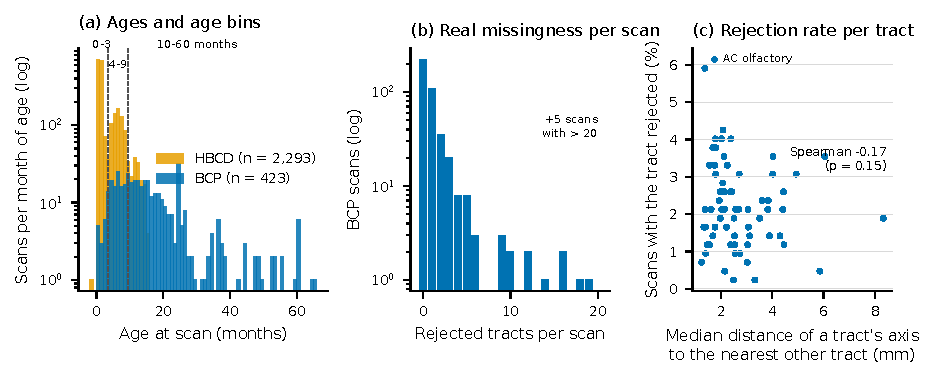
\includegraphics[width=\textwidth]{figures/fig_data.pdf}
\caption{Data. (a) Ages at scan of BCP (normative cohort) and HBCD (second cohort); dashed lines: the age bins. (b)
Real missingness of BCP after QC: number of rejected tracts per scan. (c) Per tract, the share of scans with the tract
rejected against the median distance from the tract's axis to the nearest other tract.}\label{fig:data}
\end{figure}

\subsection{Notation and norms}

For scan $s$, location $p$ (tract, arc length) and measure $m$, $y_{spm}$ is the profile value. The age-bin norm is the
mean $\mu_{bpm}$ and SD $\sigma_{bpm}$ of the cohort's scans in age bin $b$; the deviation of a scan is
$z_{spm}=(y_{spm}-\mu_{b(s)pm})/\sigma_{b(s)pm}$. Methods ``on the deviations'' impute $z$ and return
$\hat y=\mu+\sigma\hat z$ with the norm of the missing location. A continuous norm replaces the bins by a local-linear
kernel regression of each cell's mean on $\log(\text{age}+1\,\text{month})$ (bandwidth by leave-one-out
cross-validation). In validation, every norm is computed without the validated scan's subject.

\subsection{Imputation methods}\label{sec:methods}

Table~\ref{tab:methods} summarizes the method families. All are implemented in
\path{dtiplayground/dmri/fiberprofile/analysis/impute_profiles.py} (with \texttt{graph\_unet.py},
\texttt{amortized.py} and \texttt{functa.py}); the generic cohort imputers are in the scripts of this paper.

\begin{table}[t]
\centering\small
\caption{Method families and what they use. Patterns: G interior gap, E end gap, W whole profile, R region, F whole
measure family. Own: values of the scan itself; norm: age norm; cohort: models fitted on the normative cohort without
the validated subject.}\label{tab:methods}
\begin{tabular}{@{}p{3.7cm}p{1.6cm}p{7.9cm}l@{}}
\toprule
Method & Uses & Description & Patterns \\
\midrule
\multicolumn{4}{@{}l}{\textit{A. Same-scan interpolation (the scan's own values)}} \\
Arc-linear & own & linear along the arc length of the same profile; ends left, repeated or extrapolated & G, E \\
Linear (3-D), $k$NN, SIREN & own & Delaunay interpolation, inverse-distance $k$NN, or a per-scan sine network over the
3-D positions of all tracts & G, E, W, R \\
\multicolumn{4}{@{}l}{\textit{B. Norm-referenced local methods}} \\
Any method of A on $z$ & own, norm & imputes deviations from the age-bin norm & G, E, W, R \\
\multicolumn{4}{@{}l}{\textit{C. Linear population model}} \\
PPCA & own, cohort & probabilistic PCA of the deviations of all locations and measures jointly & all \\
PPCA + $k$NN / SIREN & own, cohort & a local method imputes the PPCA residuals within 4\,mm; PPCA beyond & all \\
\multicolumn{4}{@{}l}{\textit{D. Generic cohort imputers (deviation matrix, scans $\times$ 37,716 cells)}} \\
Scan offset & own, norm & the scan's mean observed deviation (per measure, or of the 5 nearest tracts) & all \\
$k$NN across scans, iterative SVD, MICE & own, cohort & as \texttt{KNNImputer}, hard-impute with ridge projection,
chained equations on tract means & all \\
\multicolumn{4}{@{}l}{\textit{E. Amortized networks (hybrid: correct the PPCA prediction)}} \\
Graph U-Net & own, cohort & multi-resolution graph convolutional U-Net over the locations & all \\
Transformer & own, cohort & masked autoencoder over patches of 8 locations, global attention & all \\
\multicolumn{4}{@{}l}{\textit{F. Blends}} \\
Fixed, precision, table & own, cohort & $(1-w)\,\hat y_{\mathrm{PPCA+local}}+w\,\hat y_{\mathrm{network}}$ & all \\
\multicolumn{4}{@{}l}{\textit{G. Explored and not adopted}} \\
Functa, partial VAE, age-dependent PPCA, acquisition correction & own, cohort & see text & all \\
\bottomrule
\end{tabular}
\end{table}

\paragraph{A. Same-scan interpolation.} \emph{Arc-linear} interpolates linearly along the arc length between the
observed values at both ends of a gap (up to 15\,mm); missing ends are left, filled with the nearest observed value
(\emph{constant}) or extrapolated from the three nearest. \emph{Linear} interpolates barycentrically within the Delaunay
tetrahedra of the observed 3-D positions of the same measure in all tracts. \emph{$k$NN} averages the $k$ nearest
observed positions with inverse-distance weights. \emph{SIREN} \citep{sitzmann2020siren} fits, per scan, a sine network
(3 hidden layers of 256 units, Adam, learning rate $10^{-4}$; \citealp{kingma2015adam}) to all observed values of all
measures jointly, each standardized within the scan, from the 3-D position (\emph{xyz}), optionally with the arc length
or a one-hot tract code; $\omega_0\in\{5,10,20,30\}$ and 100--1000 epochs were tested (Appendix
Fig.~\ref{fig:sirengrid}).

\paragraph{B. Norm-referenced local methods.} The same methods applied to $z$. Values farther than 20\,mm from any
observed value of the same measure are left to the age-bin mean.

\paragraph{C. Linear population model.} The deviations of the normative scans over all locations and measures jointly
($5{,}388\times7$ cells observed in at least 10 scans) are modelled by PPCA \citep{tipping1999ppca},
$\mathbf z=\boldsymbol\mu+W\mathbf x+\boldsymbol\epsilon$, $\mathbf x\sim\mathcal N(0,I_q)$,
$\boldsymbol\epsilon\sim\mathcal N(0,\psi I)$, fitted by EM with the exact posterior of every row
\citep{ilin2010pca}, a ridge prior on the rows of $W$, and $q=80$ components (5--160 tested; isotropic, per-measure and
per-cell noise tested, Appendix Table~\ref{tab:noise}). A scan's observed deviations give the posterior mean and SD of
every missing cell, including all cells of a family the scan lacks. The posterior SDs are rescaled per measure so that
errors on held-out whole profiles (5 folds by subject) have unit root-mean-square $z$. In \emph{PPCA + local}, the PPCA
prediction serves as the scan's own norm, and SIREN (xyz, $\omega_0=10$, 500 epochs) or $k$NN ($k=20$) imputes the
residuals within 4\,mm of an observed value; beyond, the PPCA prediction is used. PPCA + SIREN was the default of
DTIPlayground up to version 0.9.5.

\paragraph{D. Generic cohort imputers.} To place PPCA among standard tools, we evaluated, on the same hidden values and
the same training scans per fold: the \emph{scan offset} (the norm plus the scan's mean observed deviation of the
measure, or of the measure in the 5 tracts whose axis centroids are nearest to the missing tract); \emph{$k$NN across
scans} \citep{troyanskaya2001knn} (inverse-distance-weighted mean deviation of the $k\in\{5,10,20,50\}$ training scans
nearest in nan-Euclidean distance over the co-observed cells, as scikit-learn's \texttt{KNNImputer}); \emph{iterative
SVD} (hard-impute of rank $r\in\{10,40,80,160\}$ on the training deviations, a scan's missing cells from a ridge
projection of its observed cells on the loadings; cf.\ \citealp{mazumder2010softimpute}); and \emph{MICE}
\citep{vanbuuren2011mice} (\texttt{IterativeImputer}, Bayesian ridge, 40 nearest features) on the tract-mean deviations
($69\times7$ columns; MICE on 37,716 columns is impractical), whose imputed tract mean is assigned to every location of
a hidden tract.

\paragraph{E. Amortized networks.} Both networks receive per location the observed deviations (0 where missing), the
observation mask, the 3-D position and the arc length, and, in the \emph{hybrid} variant used throughout, the PPCA
prediction and its log SD; they output a mean and log variance per location and measure and correct the PPCA
prediction. They are trained on the normative cohort with the hiding patterns of Section~\ref{sec:protocol} drawn anew
in every epoch (a region in half of the scans, a whole family in a quarter), on the Gaussian negative log-likelihood of
the hidden values \citep{kendall2017uncertainties} (visible values with weight 0.1), with AdamW
\citep{loshchilov2019adamw}, a cosine schedule and batches of 16 scans; 10\% of the training subjects select the epoch and
calibrate the SDs, and the PPCA input of a training scan comes from a model fitted without its subject. The
\emph{graph U-Net}, after CONFETTI \citep{confetti}, uses a 4-level graph that keeps every $2^L$-th location of each tract
at level $L$, links nodes along the tract and to the closest node of each other tract within 1.5 times the median
distance to the nearest other tract's axis, and a U-Net \citep{gao2019graphunet} of graph convolutions \citep{kipf2017gcn}
(128 features, one convolution per level) with a scan-wide summary at the coarsest level; 60 epochs. CONFETTI's own
configuration (graph from the dense fibers, 64 features, no summary) imputed poorly (Appendix
Table~\ref{tab:confetti}). The \emph{transformer} \citep{vaswani2017attention,he2022mae} cuts each tract into patches of
8 consecutive locations (about 700 tokens per scan); a token embeds the inputs of its patch plus a tract embedding; 6
pre-norm self-attention layers of width 192 (6 heads, dropout 0.1) relate every token to every other, and a linear head
returns a mean and log variance for every location of the patch. It is trained for 200 or 400 epochs (learning rate
$10^{-3}$).

\paragraph{F. Blends.} The PPCA + local prediction $b$ and a network prediction $g$ are combined as $(1-w)b+wg$, with
(i) fixed weights $w_{\text{near}}$ for cells within 4\,mm (those the local method fills) and $w_{\text{beyond}}$ for the
others; (ii) precision weights $w=\sigma_b^{-2}/(\sigma_b^{-2}+\sigma_g^{-2})$; or (iii) a \emph{weight table} per measure
$m$ and band $k$ of the distance to the nearest observed value of the measure (0--0.5, 0.5--1, 1--2, 2--3, 3--4\,mm for
local cells; 4--6, 6--10, 10--20, $>$20\,mm for fallback cells; and a measure the scan has no observed value of). With
deviations in units of the age-bin SD, $t_i=(y_i-\mu_i)/\sigma_i$ the hidden truth and $b_i$, $g_i$ the two predictions
of hidden cell $i$, the table is the weighted least-squares solution
\begin{equation}
w_{mk}=\operatorname{clip}_{[0,1]}\frac{\sum_{i\in(m,k)}c_i\,(t_i-b_i)(g_i-b_i)}{\sum_{i\in(m,k)}c_i\,(g_i-b_i)^2},
\end{equation}
where $c_i$ is the inverse mean squared error of the age-bin mean in the cell's (pattern, measure, age bin) group,
computed on the same training cells, so that each group counts as in the score (constrained stacking;
\citealp{wolpert1992stacked,breiman1996stacked}). The table shipped with DTIPlayground 0.9.8 (``shipped'') was fitted
on all validation cells of seeds 0--2 with SIREN as the local method; scores on seeds 0--2 are cross-fitted (weights
for a scan fitted without its subject, 5 folds). The SD of a blended value is $\sqrt{(1-w)\sigma_b^2+w\sigma_g^2}$, where
$\sigma_b$ is the PPCA posterior SD (also for values filled by the local method). The released default of 0.9.8 is
PPCA + SIREN blended with a 400-epoch transformer by the shipped table.

\paragraph{Second cohort.} With \path{--transformer-reference-dir}, HBCD is batch-corrected to BCP and added to the
training of the transformer only: the transformer is trained on the pooled scans with the deviations from their pooled
age-bin norm and the pooled PPCA prediction as input, while the base prediction (norm, PPCA and SIREN) of a BCP scan
remains that of BCP. The batch correction maps each cell to BCP by one shift and scale at the same age (a spline age
curve with a shift per cohort, fitted jointly; the scale from the residual SDs over the common age range).
Alternatively the cohorts can be pooled for the norm, the PPCA and the transformer.

\paragraph{G. Explored and not adopted.} \emph{Functa} \citep{dupont2022functa,friedrich2025medfuncta}: a shared SIREN
modulated per scan by shifts from a latent vector fitted by meta-learned gradient steps; we varied inner steps and step
sizes, test-time refinement, an encoder start, depth (2--8), width (64--512), latent size (16--512), age and tract
inputs, and graph variants, on the deviations and as a hybrid. \emph{Partial VAE} \citep{ma2019eddi,mattei2019miwae}: a
set encoder of the observed cells, a latent of 32--128, a per-location decoder. \emph{Age-dependent PPCA}: a PPCA per
age with kernel weights of log age. \emph{Acquisition correction}: an offset per acquisition label and cell, fitted on
the deviations with a random intercept per subject, removed before imputation. \emph{Context inputs} to the
transformer (distance to the nearest observed value, age and acquisition) and \emph{seed ensembles} (three
transformers averaged; \citealp{lakshminarayanan2017ensembles}). The tuning budget per family is in Appendix
Table~\ref{tab:budget}.

\subsection{Evaluation protocol}\label{sec:protocol}

\paragraph{Hiding patterns.} Observed values are hidden, imputed and compared with the truth (Fig.~\ref{fig:patterns}).
Validated scans must have at least 50\% of each measure observed and at most 50\% of their tracts missing; only observed
values are hidden. (\nValidatedWithMissing{} of the \nScansDistinct{} scans validated in seeds 0--2 had real missing values.) Each validated scan goes through three rounds, each with up to four passes on the scan:
(1) whole profiles (all measures) of 10\% of the tracts with at least three observed locations; of the other tracts, an
interior gap of 3--15\,mm in 20\% (\emph{gap}) and the first or last 1--8\,mm in another 20\% (\emph{end gap}); (2) every
tract with an observed location inside a sphere of radius 10--25\,mm around a random observed location loses its whole
profile (\emph{region}; spheres reaching more than half of the tracts are redrawn); (3) all values of one measure family
the scan has, the tensor family (FA, MD, RD, AD) or the NODDI family (NDI, ODI, FWF) (\emph{whole family}); and, in the
runs of Sections~\ref{sec:e1}--\ref{sec:pooling}, (4) the real missing cells of a randomly drawn donor, a BCP scan with
missing values of the same age bin and another subject (\emph{real mask}; \path{--validate-real-masks}; donor draws
from their own random stream, so that passes 1--3 are unchanged). The hidden load of pass 1 (about 7 whole tracts and
gaps in 40\% of the other tracts) is much larger than that of the median real scan (1 rejected tract); the real-mask pass
has the real load. The hiding is identical for all settings of a run and across runs with the same seed.

\begin{figure}[t]
\centering
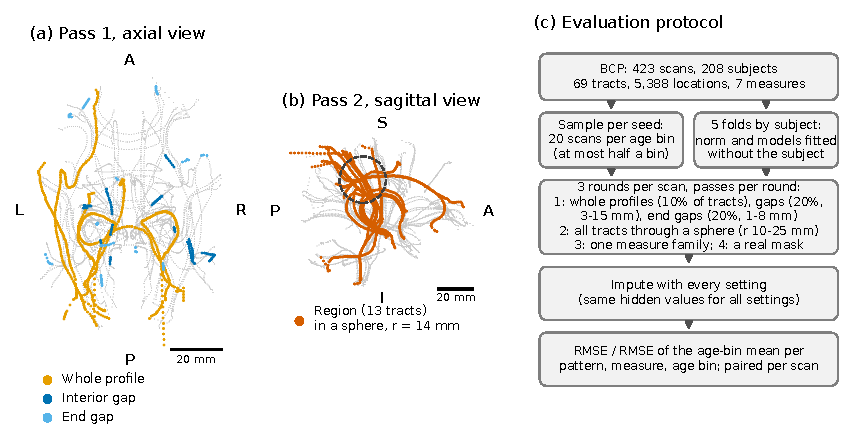
\includegraphics[width=\textwidth]{figures/fig_patterns.pdf}
\caption{Missingness patterns and evaluation protocol. (a, b) One round on a 12-month BCP scan, the profile locations
projected on axial and sagittal planes in atlas space (grey: observed; L/R, A/P, S/I: orientation; neurological
convention). (a) Pass 1 hides whole profiles of random tracts, interior gaps and end gaps; (b) pass 2 hides all
tracts through a sphere (dashed; this draw: radius as shown, 13 of 69 tracts, the median of the validation). Passes 3 (a
measure family) and 4 (a real mask) not shown. (c) The protocol.}\label{fig:patterns}
\end{figure}

\paragraph{Sampling and folds.} Per random seed (0, 1, 2), 20 scans per age bin were drawn, at most half of a bin
(\nScansBinA{}, \nScansBinB{} and \nScansBinC{}: \nScansSeed{} scans), \nScansDistinct{} distinct scans of
\nSubjDistinct{} subjects over the three seeds, \nPairs{} scan $\times$ seed pairs. Every model fitted on the cohort
(norm, PPCA, continuous norms, batch correction, networks, blend weights, generic imputers) is fitted without the
validated subjects: the validated scans are split by subject into 5 folds and each fold's models are fitted on all
other subjects.

\paragraph{Untouched test (E1).} All design choices (patterns, hyperparameters, blend variants, the shipped weight table)
were made on seeds 0--2. For an unbiased estimate, three further draws (seeds 3--5) were restricted to subjects never
validated in seeds 0--2 (\path{--validate-exclude-subjects}), with the shipped table scored as released. Only 168
eligible scans remain, so each draw validates \eOneScansBinA{}, \eOneScansBinB{} and \eOneScansBinC{} scans in the
three bins: the 0--3 month bin is essentially exhausted and E1 speaks for 4--60 months.

\paragraph{Second cohort as a test (E3).} The same protocol on HBCD alone (seeds 0--2, 20 scans per bin), with all
models fitted on HBCD folds, the transformer trained for 200 epochs (GPU budget for a cohort six times larger; 200 is
also the validated setting with a reference cohort), the shipped BCP weight table, and a table refitted on HBCD
(cross-fitted).

\paragraph{Pooling decomposition (E5).} On the BCP scans of seeds 0--2, pooled with HBCD (batch-corrected to BCP):
(i) pooled norm with a BCP-only PPCA (\path{--validate-model-batches}); (ii) BCP norm with a pooled PPCA, the HBCD
deviations relative to the BCP norm (\path{--validate-norm-batches}); (iii) both pooled with the age-bin norm and with
the kernel norm; compared with BCP alone on the same scans.

\paragraph{Score.} For a setting, pattern $P$, measure $m$ and age bin $b$, the RMSE over the hidden values is divided by
the RMSE of the age-bin mean on the same values,
\begin{equation}
\ratio_{Pmb}=\mathrm{RMSE}_{Pmb}(\text{setting})/\mathrm{RMSE}_{Pmb}(\text{age-bin mean}),
\end{equation}
so that $\ratio<1$ is better than the norm. Values a setting leaves unfilled count
with the age-bin mean. The pattern score is the mean of $\ratio$ over measures and age bins; the \emph{overall} score is
the mean over gap, end gap, whole profile and region. Because the overall score gives half its weight to gaps and end
gaps, which are \realShareEnd\% + \realShareGap\% of the real missing cells, we also report a \emph{real-weighted} score
(the pattern scores weighted by the real shares of missing cells, which is essentially the whole-profile score) and the
real-mask pattern. As a reference-independent check we report the ratios relative to the leave-subject-out kernel age
norm and absolute RMSEs (Appendix).

\paragraph{Paired statistics.} The per-scan score is the mean over pattern $\times$ measure of
$\sqrt{\mathrm{MSE}/\mathrm{MSE}_{\mathrm{norm}}}$ of that scan ($\mathrm{MSE}_{\mathrm{norm}}$: of the age-bin mean). Two settings A (reference) and B are compared by
the geometric mean over scan $\times$ seed pairs of the ratio of their per-scan scores, with a 95\% CI from a cluster
bootstrap that resamples subjects (4,000 resamples; \citealp{field2007bootstrap}), since seeds share scans and subjects
share sessions; we also give the normal-theory CI over pairs, the Wilcoxon signed-rank test \citep{wilcoxon1945} on
per-subject mean log ratios, Holm adjustment \citep{holm1979} over the \nContrasts{} contrasts of
Appendix Table~\ref{tab:paired} (selected after the development, not pre-specified), and the share of pairs in which B is better.
For claims of ``no difference'' we use an equivalence margin of $\pm2\%$: a contrast is called equivalent when its
bootstrap CI lies within 0.98--1.02 \citep{lakens2017equivalence}. These intervals reflect the sampling of scans and
hidden values, not the variation from network training (one network per fold and seed). Paired tests are only reported
between settings that fill every hidden value.

\paragraph{Quick screens.} Model families that did not justify a full validation (functa, partial VAE, age-dependent
PPCA) and transformer variants were screened on one fixed held-out split (30 test subjects, two rounds, models fitted
on the other subjects), scored like the validation. The best configuration of a family is selected on the test split
itself, which favours the family; screen numbers are comparable within the screen only.

\paragraph{Downstream analyses (E4).} To quantify what imputation does to typical analyses, we used the
\bcpscans{}-scan cohort's 220 scans without any missing value (133 subjects, 5 folds by subject). For fold $k$, the age-bin
norm and a transformer (0.9.8 settings, 400 epochs) were fitted on all BCP scans except those of fold $k$'s subjects. The
PPCA used for imputation is the transformer's hybrid-input PPCA ($q=80$) saved with it: it was fitted on the transformer's
training subjects of that fold cohort (about 90\%; its 10\% early-stopping holdout excluded), in deviations from the fold
cohort's age-bin norm, without SD calibration. For multiple imputation its posterior SDs were scaled per measure by the
factors of the population model of the default imputation run on the same fold cohort (all its scans, 5-fold
calibration), which is a close but not identical model.
In each of 50 replicates, a random half of the subjects formed group 1, and in 5 random tracts their values were shifted
by $\delta$ between-scan SDs (all locations and measures; $\delta=0.3$, and 0.1 in a second scenario); each scan then
received the real missingness of a random donor (a BCP scan of the same age bin and another subject; about half of the
donors have missing values, as in BCP; a third scenario uses only donors with missing values). Imputers: complete case
(drop a scan with any missing value); available case (drop the scan for a tract with a missing value); age-bin mean;
PPCA; PPCA + $k$NN; the blend of PPCA + $k$NN with the fold transformer using the shipped table (whose near-observed
weights were fitted for SIREN cells); and multiple imputation with 10 draws from the calibrated PPCA posterior and
Rubin's rules \citep{rubin1987multiple}. (SIREN per scan was too slow on the CPU for 50 replicates.) Analyses, per tract
and measure (FA, MD) on the tract mean: (i) the trajectory, tract mean $\sim$ natural spline of $\log(\text{age}+1)$ with
4 df, OLS with cluster-robust (subject) SEs, on the tracts without a planted effect, compared with the same fit on the
complete data (integrated absolute bias in units of the tract mean's between-scan SD, CI width ratio, pointwise coverage
of the complete-data curve); (ii) the group effect, tract mean $\sim$ group + spline, its estimate relative to the
complete-data estimate, SE ratio, power and type I error.

\paragraph{Earlier protocols.} The methods of families A--C were first run on 30 scans, one seed and 11 measures; all were
re-run with the protocol above, and we report those runs throughout. The earlier runs are used only for the SIREN
hyperparameter grid (Appendix Fig.~\ref{fig:sirengrid}), the noise models (Appendix Table~\ref{tab:noise}) and the
pooling with continuous norms on 11 measures (Appendix Table~\ref{tab:pooling11}); the graph U-Net development runs are on
seed 0 with 11 measures (Appendix Table~\ref{tab:confetti}).

\subsection{Implementation and reproducibility}

All methods are part of DTIPlayground 0.9.8 \citep{dtiplayground} (PyTorch, \citealp{paszke2019pytorch}); the new
validation options of this revision (\path{--validate-exclude-subjects}, \path{--validate-real-masks},
\path{--validate-norm-batches}, \path{--validate-model-batches}) are in DTIPlayground 0.9.9. Each validation run is
one \path{dmrifiberprofile impute-profiles --validate} call; with \path{--validate-dump-dir} it also writes every
hidden cell with all predictions, from which the blends, the weight tables, the generic imputers and the calibration were
scored offline. A run with the population model, SIREN and one network took about 2 hours on one NVIDIA RTX A6000 GPU.
Every number, table and figure is produced from the result files by the scripts accompanying the paper.

\section{Results}

\subsection{Overview}

Table~\ref{tab:main} and Fig.~\ref{fig:progression} give the error of representative settings on the same hidden
values; Table~\ref{tab:rev} adds the real-weighted score and the reference-independent view.

\begin{table}[p]
\centering\footnotesize
\caption{Error relative to the age-bin mean (RMSE ratio $\ratio$; below 1: better) on identical hidden values, mean over
3 seeds $\times$ 54 BCP scans, 7 measures and 3 age bins. Overall: mean of the four patterns (SD between seeds).
$^{\dagger}$Leaves some hidden values, counted with the age-bin mean (families A--B never fill a whole family).
$^{\ast}$Weights cross-fitted by subject; mean of the per-seed scores (pooled over seeds: 0.567 and 0.538).}\label{tab:main}
\setlength{\tabcolsep}{4pt}
\resizebox{\textwidth}{!}{\begin{tabular}{l@{\hspace{4pt}}c@{\hspace{6pt}}cccc@{\hspace{6pt}}cc}
\toprule
 & & \multicolumn{4}{c}{Pattern} & \multicolumn{2}{c}{Whole family missing} \\
\cmidrule(lr){3-6}\cmidrule(lr){7-8}
Setting & Overall (SD) & Gap & End & Whole & Region & Tensor & NODDI \\
\midrule
\multicolumn{8}{l}{\textit{Reference}} \\
\quad Age-bin mean & 1.000 (0.000) & 1.000 & 1.000 & 1.000 & 1.000 & 1.000 & 1.000 \\
\addlinespace[2pt]
\multicolumn{8}{l}{\textit{A. Same-scan interpolation (the scan's own values)}} \\
\quad Arc-linear, constant ends$^{\dagger}$ & 0.900 (0.015) & 0.759 & 0.842 & 1.000 & 1.000 & 1.000 & 1.000 \\
\quad Linear (3-D Delaunay)$^{\dagger}$ & 1.496 (0.043) & 1.074 & 0.968 & 1.818 & 2.123 & 1.000 & 1.000 \\
\quad kNN, $k=20$$^{\dagger}$ & 1.713 (0.048) & 1.490 & 1.198 & 1.893 & 2.269 & 1.000 & 1.000 \\
\quad SIREN, xyz$^{\dagger}$ & 1.418 (0.045) & 0.780 & 0.823 & 1.831 & 2.239 & 1.000 & 1.000 \\
\quad SIREN, xyz+tract$^{\dagger}$ & 1.572 (0.057) & 0.732 & 0.812 & 2.335 & 2.408 & 1.000 & 1.000 \\
\addlinespace[2pt]
\multicolumn{8}{l}{\textit{B. Norm-referenced local methods (deviations from the age-bin norm)}} \\
\quad Arc-linear, constant ends$^{\dagger}$ & 0.750 (0.011) & 0.431 & 0.570 & 1.000 & 1.000 & 1.000 & 1.000 \\
\quad Linear (3-D Delaunay)$^{\dagger}$ & 0.733 (0.006) & 0.496 & 0.701 & 0.801 & 0.934 & 1.000 & 1.000 \\
\quad kNN, $k=20$$^{\dagger}$ & 0.755 (0.009) & 0.631 & 0.683 & 0.782 & 0.923 & 1.000 & 1.000 \\
\quad kNN, $k=50$$^{\dagger}$ & 0.759 (0.010) & 0.663 & 0.712 & 0.767 & 0.893 & 1.000 & 1.000 \\
\quad SIREN, xyz+arc$^{\dagger}$ & 0.704 (0.005) & 0.422 & 0.516 & 0.895 & 0.982 & 1.000 & 1.000 \\
\quad SIREN, xyz$^{\dagger}$ & 0.688 (0.004) & 0.442 & 0.544 & 0.814 & 0.952 & 1.000 & 1.000 \\
\addlinespace[2pt]
\multicolumn{8}{l}{\textit{C. Linear population model (PPCA, $q=80$)}} \\
\quad PPCA alone & 0.733 (0.008) & 0.685 & 0.777 & 0.713 & 0.759 & 0.696 & 0.798 \\
\quad PPCA + kNN on residuals ($\leq$4\,mm) & 0.664 (0.008) & 0.568 & 0.659 & 0.675 & 0.752 & 0.696 & 0.798 \\
\quad PPCA + SIREN on residuals ($\leq$4\,mm) & 0.614 (0.007) & 0.440 & 0.552 & 0.697 & 0.766 & 0.696 & 0.798 \\
\addlinespace[2pt]
\multicolumn{8}{l}{\textit{E. Amortized networks and F. blends: graph U-Net (hybrid)}} \\
\quad U-Net alone & 0.673 (0.008) & 0.596 & 0.686 & 0.676 & 0.735 & 0.530 & 0.703 \\
\quad U-Net + SIREN on residuals & 0.659 (0.014) & 0.485 & 0.629 & 0.741 & 0.780 & 0.530 & 0.703 \\
\quad PPCA + SIREN, U-Net beyond 4\,mm & 0.610 (0.007) & 0.436 & 0.550 & 0.697 & 0.757 & 0.530 & 0.703 \\
\addlinespace[2pt]
\multicolumn{8}{l}{\textit{E/F. Transformer (hybrid) and blends}} \\
\quad Transformer alone, 200 epochs & 0.654 (0.009) & 0.547 & 0.627 & 0.704 & 0.738 & 0.446 & 0.636 \\
\quad Transformer alone, 400 epochs & 0.632 (0.005) & 0.510 & 0.588 & 0.694 & 0.737 & 0.425 & 0.623 \\
\quad PPCA + SIREN, transformer beyond 4\,mm & 0.606 (0.008) & 0.438 & 0.542 & 0.692 & 0.750 & 0.446 & 0.636 \\
\quad Blend with U-Net, fixed 0.25/0.75 & 0.594 (0.006) & 0.435 & 0.541 & 0.665 & 0.736 & 0.540 & 0.705 \\
\quad Blend with transformer (200), fixed 0.25/0.75 & 0.582 (0.008) & 0.424 & 0.518 & 0.658 & 0.729 & 0.460 & 0.643 \\
\quad Blend with transformer (400), fixed 0.25/0.75 & 0.576 (0.006) & 0.414 & 0.509 & 0.654 & 0.726 & 0.443 & 0.630 \\
\quad Blend with transformer (400), weight table$^{\ast}$ & 0.569 (0.005) & 0.418 & 0.505 & 0.639 & 0.715 & 0.424 & 0.622 \\
\addlinespace[2pt]
\multicolumn{8}{l}{\textit{E/F. Transformer (200 epochs) trained with the HBCD reference cohort}} \\
\quad Reference transformer alone & 0.580 (0.013) & 0.456 & 0.532 & 0.633 & 0.698 & 0.432 & 0.662 \\
\quad Blend, fixed 0.25/0.75 & 0.557 (0.009) & 0.400 & 0.495 & 0.634 & 0.697 & 0.439 & 0.642 \\
\quad Blend, weight table$^{\ast}$ & 0.540 (0.010) & 0.398 & 0.481 & 0.603 & 0.678 & 0.429 & 0.645 \\
\bottomrule
\end{tabular}
}
\end{table}

\begin{table}[t]
\centering\footnotesize
\caption{Main settings by the patterns that dominate real missingness: whole profiles, regions and the real-weighted
score (pattern scores weighted by the real shares of missing cells), relative to the age-bin mean; and relative to a
leave-subject-out kernel age norm (overall, whole profiles, regions). Seeds 0--2.}\label{tab:rev}
\begin{tabular}{lccccccc}
\toprule
 & \multicolumn{3}{c}{vs age-bin mean} & \multicolumn{3}{c}{vs kernel age norm} \\
\cmidrule(lr){2-4}\cmidrule(lr){5-7}
Setting & Whole & Region & Real-weighted & Overall & Whole & Region \\
\midrule
Age-bin mean & 1.000 & 1.000 & 1.000 & 1.100 & 1.108 & 1.087 \\
Kernel age norm (alone) & 0.912 & 0.927 & 0.912 & 1.000 & 1.000 & 1.000 \\
Phase 2: SIREN on deviations & 0.814 & 0.952 & 0.814 & 0.749 & 0.893 & 1.028 \\
PPCA alone & 0.713 & 0.759 & 0.713 & 0.799 & 0.783 & 0.819 \\
PPCA + kNN & 0.675 & 0.752 & 0.675 & 0.722 & 0.740 & 0.811 \\
PPCA + SIREN & 0.697 & 0.766 & 0.697 & 0.668 & 0.765 & 0.826 \\
Graph U-Net alone & 0.676 & 0.735 & 0.676 & 0.732 & 0.742 & 0.793 \\
Transformer alone (400) & 0.694 & 0.737 & 0.693 & 0.688 & 0.761 & 0.795 \\
Blend, fixed (400) & 0.654 & 0.726 & 0.654 & 0.626 & 0.718 & 0.783 \\
Released default (table) & 0.639 & 0.715 & 0.639 & 0.619 & 0.701 & 0.771 \\
HBCD-trained transformer, table & 0.603 & 0.678 & 0.603 & 0.587 & 0.661 & 0.731 \\
\bottomrule
\end{tabular}

\end{table}

\begin{figure}[t]
\centering
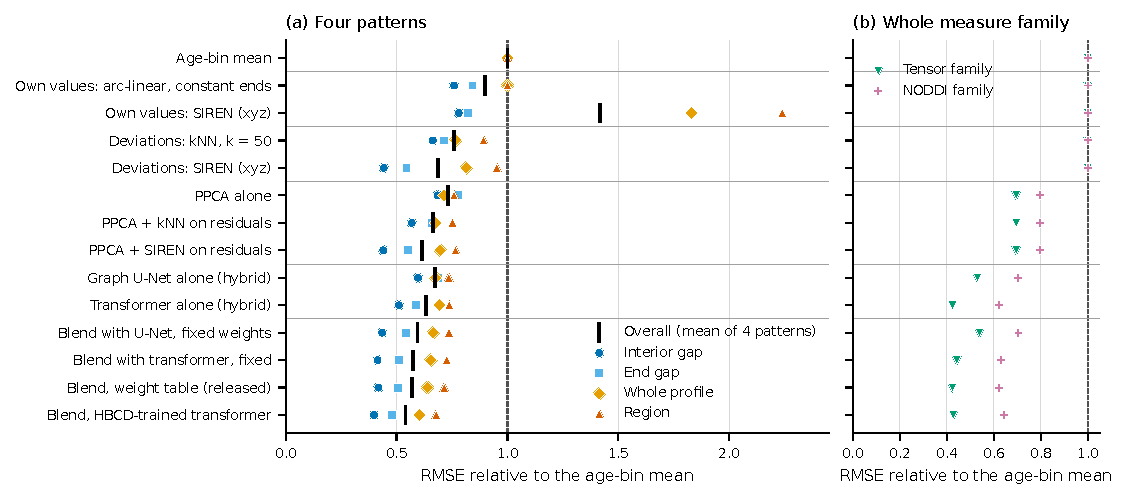
\includegraphics[width=\textwidth]{figures/fig_progression.pdf}
\caption{Error relative to the age-bin mean of representative settings, grouped by method family. (a) Per pattern
(markers) and overall (vertical bar). (b) A whole measure family hidden; same-scan and norm-referenced local methods
cannot impute it (1.0 by construction). ``Released'': the default of DTIPlayground 0.9.8 (cross-fitted).}\label{fig:progression}
\end{figure}

\paragraph{Same-scan interpolation is not enough.} From a scan's own values, only gaps and end gaps along a profile were
imputed better than the age-bin mean (arc-linear \rPoneArcGap{} and \rPoneArcEnd{} with constant ends; SIREN
\rPoneSirenGap{} and \rPoneSirenEnd{}). The 3-D methods imputed whole profiles and regions far worse than the norm
(SIREN \rPoneSirenWhole{} and \rPoneSirenRegion{}, linear \rPoneLinearWhole{} and \rPoneLinearRegion{}): a scan's
neighbouring tracts do not predict the values of a missing tract.

\paragraph{The norm makes every pattern imputable.} On the deviations from the age-bin norm, SIREN reached
\rPtwoSirenWhole{} for whole profiles and \rPtwoSirenRegion{} for regions (from \rPoneSirenWhole{} and
\rPoneSirenRegion{} on the values), and \rPtwoSiren{} overall. The norm carries the tract-specific level at the scan's
age; the neighbours then only need to carry the scan's deviation from it. Regions remained close to the norm.

\paragraph{A linear population model.} PPCA alone improved whole profiles (\rPpcaWhole) and regions (\rPpcaRegion) over
the norm-referenced local methods, and is the first method that imputes a missing measure family (tensor \rPpcaWdti,
NODDI \rPpcaWnoddi). Imputing its residuals locally helped gaps and end gaps most. Which local method is better depends
on the pattern (Table~\ref{tab:patterns}): for gaps SIREN was much better than $k$NN ($k$NN \pcAGap{} times SIREN's
error), but for whole profiles $k$NN was better (\pcAWhole, 95\% CI \pcAWholeCi, better on \pcAWholeBetter\% of scan
draws) and for regions slightly better (\pcARegion); for regions PPCA alone was as good as PPCA + SIREN (\pcBRegion).
Under the real weighting, PPCA + $k$NN (\rwPpcaKnn) is better than PPCA + SIREN (\rwDefault).

\begin{table}[t]
\centering\footnotesize
\caption{Pattern-specific paired contrasts (geometric mean ratio of per-scan errors, compared / reference, with the
95\% subject-bootstrap CI; 162 scan $\times$ seed pairs).}\label{tab:patterns}
\resizebox{\textwidth}{!}{\begin{tabular}{lcccc}
\toprule
Contrast (compared vs reference) & Whole profile & Region & Interior gap & End gap \\
\midrule
PPCA + kNN vs PPCA + SIREN & 0.965 [0.960, 0.969] & 0.981 [0.978, 0.983] & 1.325 [1.303, 1.348] & 1.187 [1.163, 1.211] \\
PPCA alone vs PPCA + SIREN & 1.026 [1.017, 1.036] & 0.990 [0.986, 0.994] & 1.608 [1.576, 1.642] & 1.406 [1.368, 1.441] \\
Transformer (400) vs PPCA + SIREN & 0.994 [0.983, 1.006] & 0.955 [0.947, 0.963] & 1.185 [1.160, 1.210] & 1.026 [0.995, 1.058] \\
U-Net vs PPCA + SIREN & 0.963 [0.953, 0.974] & 0.956 [0.948, 0.963] & 1.370 [1.341, 1.403] & 1.217 [1.187, 1.246] \\
Released default vs PPCA + SIREN & 0.915 [0.908, 0.922] & 0.929 [0.923, 0.934] & 0.952 [0.940, 0.964] & 0.907 [0.892, 0.922] \\
Released default vs PPCA + kNN & 0.949 [0.942, 0.956] & 0.947 [0.941, 0.953] & 0.718 [0.705, 0.732] & 0.764 [0.750, 0.778] \\
Released default vs PPCA alone & 0.892 [0.884, 0.900] & 0.939 [0.933, 0.944] & 0.592 [0.581, 0.604] & 0.645 [0.631, 0.660] \\
HBCD-reference blend vs released default & 0.950 [0.939, 0.960] & 0.956 [0.945, 0.966] & 0.954 [0.944, 0.965] & 0.943 [0.932, 0.956] \\
\bottomrule
\end{tabular}
}
\end{table}

\paragraph{Distance limit of the local methods.} The PPCA residuals are local. Scored from the per-distance errors of
the same cells (Appendix Table~\ref{tab:cap}), SIREN on the residuals up to 2\,mm instead of 4\,mm improved whole profiles
(\capSirenTwoWhole{} vs \capSirenFourWhole) and regions (\capSirenTwoRegion{} vs \capSirenFourRegion) but made gaps worse
(\capSirenTwoGap{} vs \capSirenFourGap); for $k$NN the 4-mm limit was better for every pattern. The 4-mm limit of SIREN is
therefore a compromise driven by the gap patterns.

\paragraph{Generic cohort imputers.} Standard imputers on the deviation matrix, with the same training scans as PPCA
(Appendix Table~\ref{tab:baselines}), were clearly worse than the population model, except for the low-rank model, which
is essentially the same model fitted differently: iterative SVD of rank \blSvdBestName{} reached \blSvdBest{} overall and
\blSvdBestWhole{} for whole profiles (paired against PPCA alone for whole profiles \blSvdPairWhole, CI
\blSvdPairWholeCi). $k$NN across scans (best $k=\blKnnBestName$: \blKnnBest{} overall, \blKnnBestWhole{} for whole
profiles; paired \blKnnPairWhole) and MICE on the tract-mean deviations (\blMice; \blMiceWhole; paired
\blMicePairWhole) were about 13--15\% worse than PPCA for whole profiles. The scan-wide offset alone (the norm plus the scan's
mean observed deviation of the measure) reached \blOffMeasureWhole{} for whole profiles (\blOffNearWhole{} using the 5
nearest tracts), that is, a scan-wide shift accounts for about \blOffShare\% of PPCA's gain over the norm on whole profiles; the rest
is the covariation of deviations across tracts and measures.

\paragraph{Amortized networks and blends.} The hybrid graph U-Net (\rUnet) and transformer (\rTfFour{} with 400 epochs)
alone were worse than PPCA + SIREN overall, because they are worse for gaps and end gaps; for whole profiles the U-Net was
better than PPCA + SIREN (paired \pcDWhole, CI \pcDWholeCi) and the transformer equivalent (\pcCWhole, CI \pcCWholeCi),
and both were better for regions (\pcDRegion, \pcCRegion; Table~\ref{tab:patterns}). Their strength is a missing family: tensor \rUnetWdti{} and \rTfFourWdti, NODDI
\rUnetWnoddi{} and \rTfFourWnoddi, against \rPpcaWdti{} and \rPpcaWnoddi{} for PPCA (paired, transformer vs PPCA for a
missing family: \wCRatio, better on \wCBetter\% of draws). Blending the networks with PPCA + SIREN combined both: a fixed
blend reached \rUnetBlend{} with the U-Net and \rTfBlendFour{} with the transformer, the weight table \rFinal{}
(cross-fitted). Against PPCA + SIREN, the released default had a paired ratio of \pcEWhole{} for whole profiles,
\pcERegion{} for regions, \pcEGap{} for gaps and \pcEEnd{} for end gaps (better on \pcEWholeBetter\%, \pcERegionBetter\%,
\pcEGapBetter\% and \pcEEndBetter\% of draws), and against PPCA + $k$NN \pcFWhole{} for whole profiles
(Table~\ref{tab:patterns}). The transformer was better than the U-Net alone (paired \cIRatio), but the U-Net had a smaller
training budget (60 epochs; Appendix Table~\ref{tab:budget}). Trained for 200 epochs on the same draws (O5), the U-Net did
not improve: alone it reached \oFiveUnet{} (paired against 60 epochs \oFiveVsSixty, CI \oFiveVsSixtyCi; the epoch with the
smallest held-out error is kept, so longer training only adds overfitting room), its fixed blend \oFiveBlend{} (60 epochs:
\rUnetBlend), and against the transformer at the same 200 epochs its error was \oFiveVsTf{} times as large (CI \oFiveVsTfCi).
The advantage of the transformer is therefore not a training-budget artefact.

\paragraph{Blend weights.} The learned weight of the transformer rose with the distance to the nearest observed value
(Fig.~\ref{fig:weights}): \wtCNearMin--\wtCNearMax{} next to an observed value, \wtCFarMin--\wtCFarMax{} for fallback
cells, \wtCFamMin--\wtCFamMax{} for a missing family. Refitting reproduced the shipped table to two decimals. The table
was better than fixed 0.25/0.75 weights with the same transformer (\cNRatio, CI \cNBci), 400 epochs better than 200
(\cMRatio, CI \cMBci); precision weights were worse (\cLRatio, CI \cLBci), because the SD attached to a locally imputed
value is that of PPCA, an upper bound next to an observed value. A gradient-boosted weight per cell and calibrated
precision weights were no better than the table (Appendix Table~\ref{tab:learners}). These differences of 1--2\% were
selected on the same draws (Section~\ref{sec:e1}).

\begin{figure}[t]
\centering
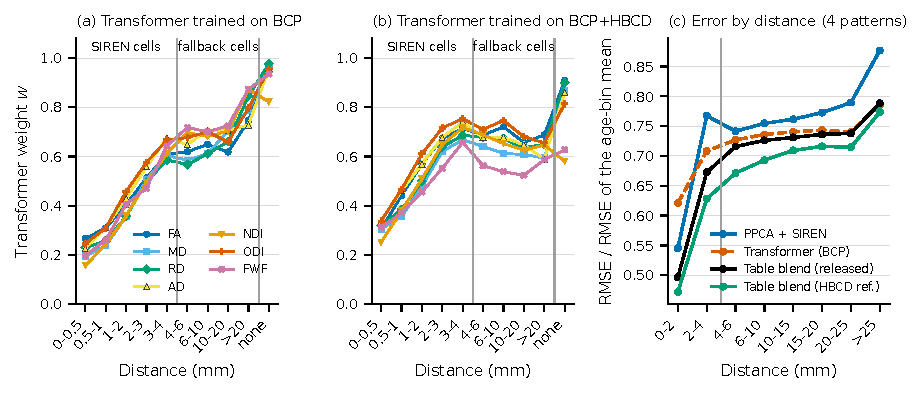
\includegraphics[width=\textwidth]{figures/fig_weights.pdf}
\caption{Blend weights. (a, b) Weight $w$ of the transformer per measure and distance band (local cells within 4\,mm,
fallback cells beyond, ``none'': no observed value of the measure), fitted on all validation cells; (a) trained on BCP
(shipped table), (b) trained on BCP and HBCD. (c) Error against distance, four patterns pooled, from the cell dumps
(distance bins as in Fig.~\ref{fig:distance}; PPCA alone is in Fig.~\ref{fig:distance}).}\label{fig:weights}
\end{figure}

\paragraph{Distance to the nearest observed value.} Within each pattern, the error grew with the distance to the nearest
observed value of the same measure (Fig.~\ref{fig:distance}). PPCA + SIREN was worse than PPCA alone at 2--4\,mm for
whole profiles and regions, where PPCA + $k$NN was not; beyond 4\,mm the networks and the blend were best.

\begin{figure}[t]
\centering
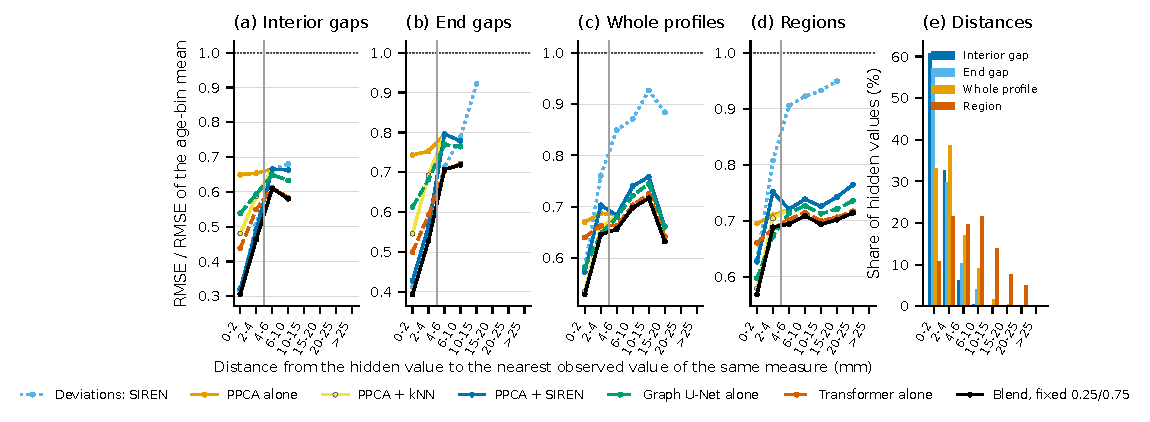
\includegraphics[width=\textwidth]{figures/fig_distance.pdf}
\caption{Error by the distance from a hidden value to the nearest observed value of the same measure, per pattern (3
seeds; bins with fewer than 600 hidden values omitted; vertical line: 4\,mm). (e) Share of hidden values per distance
bin.}\label{fig:distance}
\end{figure}

\subsection{How much does the normative reference help?}

The normative information enters at three levels. The age-bin norm turned whole profiles and regions from 1.8--2.4 times
the norm's error (same-scan 3-D methods) into 0.77--0.95 (norm-referenced local methods, Table~\ref{tab:main}). The population model, which captures how deviations co-vary
across all tracts and measures, took whole profiles to \rPpcaWhole{} and made a missing family imputable. Learned
corrections of the population prediction took whole profiles to \rFinalWhole{} (\rRefFinalWhole{} with a larger training
cohort). A continuous kernel age norm alone was \rwKernel{} of the age-bin mean's error for whole profiles, and the age-bin
mean was \rAgeMean{}\,/\,\rwKernel{} $\approx$ 1.10 of the kernel norm's (Table~\ref{tab:rev}); relative to the kernel norm
all ratios rise by about 10\% but the ranking is unchanged (whole profiles: released default \kFinalWhole{},
PPCA + $k$NN \kPpcaKnnWhole{}, PPCA + SIREN \kDefaultWhole). Under PPCA + SIREN the choice of norm made no difference
(kernel vs bins \vpKernRatio{}, CI \vpKernCi{}, 11-measure protocol, Appendix Table~\ref{tab:pooling11}): the population
model absorbs the within-bin age trend.

\subsection{Size of the normative cohort and age resolution of the norm}\label{sec:o1o3}

To see how many normative scans the population model needs (O1), the norm and the PPCA of each validation fold were fitted
on a random 25, 50, 75 or 100\% of the training subjects (on average \oNQ, \oNH, \oNT{} and \oNA{} scans), and PPCA alone
and PPCA + $k$NN were scored on the same hidden values (Appendix Table~\ref{tab:o1o3}, Fig.~\ref{fig:o1o3}; CPU fits,
\oOneSeeds{} seeds, \oOneScans{} scan $\times$ seed pairs). For whole profiles, PPCA + $k$NN reached \oQKnnWhole,
\oHKnnWhole, \oTKnnWhole{} and \oAKnnWhole{} with the four training sets; paired against the full set, the error was
\oPairQKnn{} (CI \oPairQKnnCi) times as large with about \oNQ{} scans, \oPairHKnn{} (CI \oPairHKnnCi) with about \oNH{} and
\oPairTKnn{} (CI \oPairTKnnCi) with about \oNT. The gain thus flattens above about 300 scans but has not stopped at 400,
so a larger normative cohort would still help a little. Because the norm was refitted from the same subsets, the curve
includes the effect of a noisier age-bin norm.

Finer age bins (O3; seven bins of 0--1, 2--3, 4--6, 7--9, 10--14, 15--24 and 25--65 months) made the norm alone a better
predictor (\oFNorm{} of the 3-bin mean's error overall), but under the population model they were worse than the three
bins (PPCA + $k$NN, whole profiles: \oFKnnWhole{} against \oAKnnWhole; paired \oPairFKnn, CI \oPairFKnnCi): with fewer scans
per bin, the norm's means and SDs are noisier, and the population model already absorbs the within-bin age trend (as with
the kernel norm above).

\subsection{What did not help}\label{sec:negative}

\paragraph{Functa.} Over \nFunctaConfigs{} screened runs, the best functa model reached \sFunctaHyb{} as a hybrid
correcting PPCA and \sFunctaDev{} on the deviations, against \sPpca{} for PPCA alone and \sUnet{} for the hybrid U-Net on
the same split (Appendix Table~\ref{tab:screens}, Fig.~\ref{fig:screens}). The hybrid functa is thus 2.5\% better than PPCA alone
on the screen (optimistically, being selected on that split), but half as much as the U-Net gained; it was never
combined with SIREN or blended. Fitting a per-scan latent by a few gradient steps did much worse than PPCA's exact
posterior, even with a learned vector per location that could in principle reproduce PPCA.

\paragraph{Partial VAE and age-dependent PPCA.} The partial VAE reached \sVaeHyb{} as a hybrid and \sVaeDev{} on the
deviations (4 configurations each, a small budget), no better than PPCA alone. A population model per age with kernel
weights was worse than one model of all ages (\sAgePpca--\sAgePpcaMax{} against \sPpca{}).

\paragraph{Acquisition correction.} BCP scans of the \texttt{\bcpAcqBName} acquisition deviated systematically from
\texttt{\bcpAcqAName} (FA \acqOffFA, AD \acqOffAD, NDI \acqOffNDI, ODI \acqOffODI{} SD, fitted with a random intercept per
subject), and the two acquisitions are unevenly distributed over the age bins (Appendix Table~\ref{tab:acq}). Removing
these offsets before imputation was equivalent to not removing them (paired \cPRatio, CI \cPBci). A scan-wide offset is
visible in the scan's own observed values; how much of PPCA's gain is such an offset is shown by the scan-offset baseline
above.

\paragraph{Context inputs and seed ensembles.} On seed 0 (54 scans), giving the transformer the distance to the
nearest observed value (blend, paired \xDistRatioBlend, CI \xDistCiBlend) or the age and acquisition
(\xCtxRatioBlend, \xCtxCiBlend), or averaging three transformers trained with different seeds (\xMembersRatioBlend,
\xMembersCiBlend), was equivalent within $\pm2\%$ to the plain transformer. These checks used one seed.

\subsection{Untouched test subjects}\label{sec:e1}

\begin{table}[t]
\centering\footnotesize
\caption{E1: untouched subjects (seeds 3--5; subjects of seeds 0--2 excluded; \eOneScansBinA, \eOneScansBinB{} and
\eOneScansBinC{} scans per draw in the three bins), the shipped weight table scored as released. ``Real mask'': the
fourth pass.}\label{tab:e1}
\resizebox{\textwidth}{!}{\begin{tabular}{lcccccccc}
\toprule
Setting & Overall (SD) & Gap & End & Whole & Region & Tensor & NODDI & Real mask \\
\midrule
age-bin mean & 1.000 (0.000) & 1.000 & 1.000 & 1.000 & 1.000 & 1.000 & 1.000 & 1.000 \\
PPCA alone & 0.803 (0.016) & 0.748 & 0.799 & 0.811 & 0.853 & 0.760 & 0.859 & 0.801 \\
PPCA + kNN & 0.731 (0.020) & 0.615 & 0.700 & 0.763 & 0.844 & 0.760 & 0.859 & 0.758 \\
PPCA + SIREN & 0.680 (0.015) & 0.470 & 0.603 & 0.787 & 0.861 & 0.760 & 0.859 & 0.777 \\
Transformer alone & 0.699 (0.013) & 0.569 & 0.644 & 0.778 & 0.803 & 0.480 & 0.633 & 0.757 \\
Fixed blend (SIREN base) & 0.639 (0.011) & 0.447 & 0.569 & 0.736 & 0.803 & 0.491 & 0.651 & 0.723 \\
Fixed blend (kNN base) & 0.682 (0.014) & 0.558 & 0.647 & 0.729 & 0.795 & 0.491 & 0.651 & 0.718 \\
Precision blend & 0.643 (0.015) & 0.476 & 0.565 & 0.734 & 0.796 & 0.507 & 0.679 & 0.724 \\
Shipped table (SIREN base; released default) & 0.633 (0.012) & 0.456 & 0.563 & 0.723 & 0.789 & 0.479 & 0.636 & 0.713 \\
Shipped table (kNN base) & 0.670 (0.015) & 0.541 & 0.625 & 0.725 & 0.787 & 0.479 & 0.636 & 0.716 \\
\bottomrule
\end{tabular}
}
\end{table}

On subjects never used for any design decision (Table~\ref{tab:e1}; \eOnePairs{} scan $\times$ seed pairs of
\eOneSubjects{} subjects), the conclusions held. The released default had a paired ratio of \eOneFinalVsDef{} (CI
\eOneFinalVsDefCi, better on \eOneFinalVsDefBetter\% of draws) against PPCA + SIREN, against \cORatio{} on the
development draws; for whole profiles \eOneFinalVsDefWhole{} (CI \eOneFinalVsDefWholeCi; development \pcEWhole). The
ranking for whole profiles was unchanged: released default \eOneFinalWhole, PPCA + $k$NN \eOneKnnWhole, PPCA + SIREN
\eOneDefWhole, PPCA alone \eOnePpcaWhole{} (PPCA + $k$NN vs PPCA + SIREN \eOneKnnVsDefWhole, CI \eOneKnnVsDefWholeCi;
development \pcAWhole), and SIREN remained much better for gaps (\eOneKnnVsDefGap{} for $k$NN). The shipped weight table
was again slightly better than fixed weights (\eOneFinalVsFixed, CI \eOneFinalVsFixedCi). Blending the transformer with
PPCA + $k$NN instead of PPCA + SIREN, with the same table, gave \eOneFinalKnnVsKnn{} of PPCA + $k$NN's error (CI
\eOneFinalKnnVsKnnCi). All ratios to the age-bin mean were higher than on the development draws (released default
\eOneFinal{} overall, \eOneFinalOverallBC{} at 4--60 months; PPCA + SIREN \eOneDef{} and \eOneDefOverallBC); the
untouched scans are those left after the development draws and lie farther from their bin means, but the relative gains
between methods, which the paired ratios measure, reproduced within 0.002. The 0--3 month bin had only
\eOneScansBinA{} scan per draw, so E1 speaks for 4--60 months. A weight table refitted on the untouched cells (cross-fitted) gave the same error as
the shipped table (\eOneRefitDump{} vs \eOneShippedDump), so the shipped weights are not overfitted to the development
draws. Relative to the kernel age norm, which on these scans was \eOneKernelAlone{} of the age-bin mean's error, the released
default reached \eOneKFinal{} overall and \eOneKFinalWhole{} for whole profiles (PPCA + $k$NN \eOneKKnnWhole, PPCA + SIREN
\eOneKDefWhole). Its SDs were calibrated as on the development draws (RMS error/SD \eOneCalWhole{} for whole profiles,
\eOneCalWholeCov\% within 1.96 SD; \eOneCalReal{} and \eOneCalRealCov\% for real masks).

\subsection{Realistic missingness}\label{sec:real}

With the real missing cells of other scans as the hidden values (Table~\ref{tab:real}, Appendix
Table~\ref{tab:realall}; untouched subjects), the errors were close to those of whole profiles, as expected from the real
missingness. Unlike the per-scan paired ratios, this score is cell-weighted: donors with many rejected tracts contribute
most of its cells. The validation draws donors from every scan with missing values, including the few that miss more
than half of their tracts and would not be imputed by \path{impute-profiles} (\path{--max-missing-tracts}~0.5); we
recovered the donor of every pass (by replaying the validation's random draws, verified against the hidden cells) and
report both all donors and donors within the tool's scope. For BCP the restriction hardly matters (\rmOneOutPasses{} of
\rmOnePasses{} passes; released default \rmOneFinalIn{} instead of \rmOneFinalAll). With all donors, the released default had
\eOneFinalReal{} of the age-bin mean's error, PPCA + $k$NN \eOneKnnReal, PPCA + SIREN \eOneDefReal{} and PPCA alone
\eOnePpcaReal. Paired, the released default was \eOneFinalVsDefReal{} of PPCA + SIREN's error (CI \eOneFinalVsDefRealCi,
better on \eOneFinalVsDefRealBetter\% of draws) and \eOneFinalVsKnnReal{} of PPCA + $k$NN's (CI \eOneFinalVsKnnRealCi);
PPCA + $k$NN was \eOneKnnVsDefReal{} of PPCA + SIREN's (CI \eOneKnnVsDefRealCi), and PPCA alone \eOnePpcaVsDefReal{} (CI
\eOnePpcaVsDefRealCi). The realistic masks thus confirm the ranking derived from the whole-profile pattern: released
default, then PPCA + $k$NN, then PPCA + SIREN. In BCP the error depended little on how much of the scan was hidden
(Fig.~\ref{fig:realmask}a; Appendix Table~\ref{tab:realload}). In the development results, weighting the four patterns by the real
frequencies amounts to the whole-profile score (Table~\ref{tab:rev}); weighting the whole-profile
error of each tract by its real rejection rate changed the released default's error from \trUFinal{} (unweighted mean
over tracts) to \trWFinal{}, since the per-tract error is unrelated to the rejection rate (Spearman \trRhoRej, $p =
\trRhoRejP$). In regions, the error grew with the number of tracts hidden together (released default \loadFinalA{} for
1--5 tracts to \loadFinalE{} for more than 20; PPCA + SIREN \loadDefaultA{} to \loadDefaultE).

\begin{table}[t]
\centering\footnotesize
\caption{E2: error relative to the age-bin mean for the real-mask pattern (the real missing cells of a donor scan of the
same age bin and another subject), with all donors and with the donors that \texttt{impute-profiles} would impute (at most
half of their tracts missing). Cell dumps of E1 (seeds 3--5) and E3 (seeds 0--2); PPCA alone and the pooled runs are not
in the dumps (all donors: Appendix Table~\ref{tab:realall}).}\label{tab:real}
\resizebox{\textwidth}{!}{\begin{tabular}{lcccc}
\toprule
 & \multicolumn{2}{c}{BCP, untouched subjects (E1)} & \multicolumn{2}{c}{HBCD (E3)} \\
\cmidrule(lr){2-3}\cmidrule(lr){4-5}
Setting & all donors & donors $\leq$50\% tracts missing & all donors & donors $\leq$50\% tracts missing \\
\midrule
Age-bin mean & 1.000 & 1.000 & 1.000 & 1.000 \\
PPCA + $k$NN & 0.758 & 0.752 & 1.083 & 0.973 \\
PPCA + SIREN & 0.777 & 0.771 & 1.086 & 0.975 \\
Transformer alone & 0.757 & 0.754 & 0.767 & 0.743 \\
Fixed blend (SIREN base) & 0.723 & 0.718 & 0.816 & 0.786 \\
Shipped table (released default) & 0.713 & 0.708 & 0.799 & 0.768 \\
Shipped table ($k$NN base) & 0.716 & 0.712 & 0.805 & 0.775 \\
Table refitted on the cohort (cross-fitted) & 0.712 & 0.707 & 0.764 & 0.737 \\
\bottomrule
\end{tabular}
}
\end{table}

\begin{figure}[t]
\centering
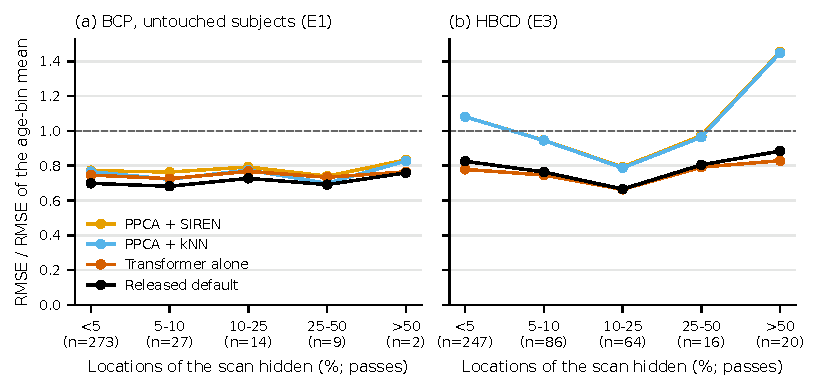
\includegraphics[width=0.85\textwidth]{figures/fig_realmask.pdf}
\caption{Real-mask pattern: error relative to the age-bin mean against the share of the scan's 5,388 locations hidden
(passes per class in parentheses). Above 50\%, nearly all donors are outside the scope of \texttt{impute-profiles}.
(a) BCP, untouched subjects (E1); (b) HBCD (E3).}\label{fig:realmask}
\end{figure}

\subsection{A second cohort}\label{sec:pooling}

\paragraph{HBCD as a test cohort (E3).} On HBCD alone (Table~\ref{tab:e3}; \eThreePairs{} scan $\times$ seed pairs of
\eThreeSubjects{} subjects; every model fitted on HBCD folds, the transformer trained for 200 epochs, the shipped BCP weight
table), the main conclusions transferred, with two differences. The released default had \eThreeFinalVsDef{} of PPCA +
SIREN's error (CI \eThreeFinalVsDefCi; BCP \cORatio), \eThreeFinalVsDefWhole{} for whole profiles and
\eThreeFinalVsDefReal{} for the real masks of HBCD (CI \eThreeFinalVsDefRealCi). PPCA + $k$NN was again slightly better than
PPCA + SIREN for whole profiles (\eThreeKnnVsDefWhole, CI \eThreeKnnVsDefWholeCi) and real masks (\eThreeKnnVsDefReal) and
much worse for gaps (\eThreeKnnVsDefGap), and the shipped table again beat fixed weights (\eThreeFinalVsFixed). The
differences: first, the population model gained little for regions (\eThreeDefRegion{} for PPCA + SIREN, \eThreeKnnRegion{}
for PPCA + $k$NN) and for the real masks of HBCD. HBCD's missingness is heavier and more clustered than BCP's
(Table~\ref{tab:data}: \hbcdMissCells\% of the cells missing vs \bcpMissCells\%, median \hbcdMissMed{} rejected tracts per
affected scan vs \bcpMissMed), and its real-mask passes hid about twice as much (median \rmThreeHiddenMedian{} locations vs
\rmOneHiddenMedian{} in BCP; mean \rmThreeHiddenMean{} vs \rmOneHiddenMean). \rmThreeOutPasses{} of \rmThreePasses{} HBCD
passes (\rmThreeOutPassShare\%) used a donor outside the scope of \path{impute-profiles}, hiding up to \rmThreeMaxHidden\% of
the scan, and they held \rmThreeOutCellShare\% of the real-mask cells. With all donors, PPCA + SIREN was worse than the
age-bin mean (\rmThreeDefAll); with the donors in scope it reached \rmThreeDefIn{} (PPCA + $k$NN \rmThreeKnnIn): a small gain,
not a failure. The population model was clearly worse than the norm when most of the scan was hidden
(Fig.~\ref{fig:realmask}b; \rmThreeShareEDef{} above 50\%), which the default \path{--max-missing-tracts}~0.5 excludes
(the 0.5 default is thus needed for the PPCA-based settings and sufficient on BCP), and above the norm's error for the
smallest masks (\rmThreeShareADef{} when less than 5\% was hidden, \rmThreeSharePassesA{} of \rmThreePasses{} passes;
\rmThreeLoadADef{} for single-tract donors). These cell-weighted points are driven by a minority of scans with large
errors (heavy tails): per scan on the passes hiding less than 5\%, PPCA + SIREN had \rmThreeScanSmallDef{} of the norm's
error (CI \rmThreeScanSmallDefCi) but was better on only \rmThreeScanSmallDefBetter\% of scans, against
\rmThreeScanSmallTfBetter\% for the transformer (\rmThreeScanSmallTf) and \rmThreeScanSmallFinalBetter\% for the
released default (\rmThreeScanSmallFinal); over all passes in scope it had \rmThreeScanInDef{} (CI \rmThreeScanInDefCi),
better on \rmThreeScanInDefBetter\% of scans. The cell-weighted scores of the intermediate classes (\rmThreeShareBDef,
\rmThreeShareCDef{} and \rmThreeShareDDef{} for 5--10, 10--25 and 25--50\% hidden; \rmThreeSharePassesB,
\rmThreeSharePassesC{} and \rmThreeSharePassesD{} passes) should not be read as a U-shaped dependence on load: they rest
on few passes and are dominated by the same tails. Second, the transformer, trained
on six times as many scans as in BCP, was much stronger and robust to the load: alone it reached \eThreeTf{} overall (BCP,
400 epochs: \rTfFour), \eThreeTfRegion{} for regions and \rmThreeTfIn{} for the real masks in scope (\rmThreeShareETf{} above
50\% hidden). The blends remained best for the synthetic patterns, including whole profiles (shipped table
\eThreeFinalWhole{} vs \eThreeTfWhole{} for the transformer alone; fixed blend \eThreeFixedWhole). For regions and the real
masks, the transformer alone matched or beat the blend with the shipped BCP table (real masks in scope \rmThreeTfIn{} vs
\rmThreeFinalIn; per scan \rmThreeTfVsFinal, CI \rmThreeTfVsFinalCi), but a weight table refitted on HBCD (cross-fitted)
matched or beat it: \eThreeRefit{} overall against \eThreeShippedDump{} for the shipped table on the same cells, and
\rmThreeRefitIn{} on the real masks in scope (per scan \rmThreeRefitVsTf{} of the transformer alone's error, CI
\rmThreeRefitVsTfCi). Refitted on the target cohort, the table gives the stronger transformer more weight where it is
better.

\begin{table}[t]
\centering\footnotesize
\caption{E3: HBCD alone (seeds 0--2, 20 scans per bin; transformer 200 epochs; shipped BCP weight table). Real mask:
all donors (donors in the tool's scope: Table~\ref{tab:real}).}\label{tab:e3}
\resizebox{\textwidth}{!}{\begin{tabular}{lcccccccc}
\toprule
Setting & Overall (SD) & Gap & End & Whole & Region & Tensor & NODDI & Real mask \\
\midrule
age-bin mean & 1.000 (0.000) & 1.000 & 1.000 & 1.000 & 1.000 & 1.000 & 1.000 & 1.000 \\
PPCA alone & 0.776 (0.020) & 0.681 & 0.717 & 0.727 & 0.981 & 0.628 & 0.757 & 1.097 \\
PPCA + kNN & 0.703 (0.018) & 0.557 & 0.602 & 0.682 & 0.970 & 0.628 & 0.757 & 1.083 \\
PPCA + SIREN & 0.644 (0.025) & 0.409 & 0.499 & 0.690 & 0.978 & 0.628 & 0.757 & 1.086 \\
Transformer alone & 0.578 (0.004) & 0.463 & 0.481 & 0.630 & 0.740 & 0.341 & 0.516 & 0.767 \\
Fixed blend (SIREN base) & 0.559 (0.006) & 0.385 & 0.454 & 0.631 & 0.766 & 0.364 & 0.536 & 0.816 \\
Fixed blend (kNN base) & 0.609 (0.000) & 0.498 & 0.538 & 0.635 & 0.763 & 0.364 & 0.536 & 0.818 \\
Precision blend & 0.578 (0.013) & 0.401 & 0.444 & 0.629 & 0.841 & 0.375 & 0.563 & 0.901 \\
Shipped table (SIREN base; released default) & 0.550 (0.004) & 0.389 & 0.444 & 0.612 & 0.756 & 0.341 & 0.519 & 0.799 \\
Shipped table (kNN base) & 0.592 (0.001) & 0.476 & 0.511 & 0.622 & 0.757 & 0.341 & 0.519 & 0.805 \\
\bottomrule
\end{tabular}
}
\end{table}

\paragraph{Pooling depends on age.} Pooling HBCD into the norm and population model of BCP (batch-corrected) made PPCA +
SIREN worse overall (\pbAAll; Appendix Table~\ref{tab:poolbins}), but not uniformly: it tended to help at 0--3 months (\pbAA),
where BCP has \bcpbinA{} scans and HBCD \hbcdbinA, and hurt at 4--9 (\pbAB) and 10--60 months (\pbAC), where HBCD is
sparse or differs in age composition within the bins. The fully pooled fixed blend (pooled norm, PPCA and transformer;
\rPooledBlend) was equivalent to the released BCP-only default (\pbBAll), better at 0--3 months (\pbBA), and 1.6\% worse
than training only the transformer on both cohorts (\pbCAll). At equal training length (200 epochs), the transformer
trained on BCP + HBCD was \pbDAll{} of the BCP transformer's error alone, and \pbEAll{} within the fixed blend; the gain
was largest at 0--3 months (\pbDA). 

\paragraph{Pooling the population model, not the norm, causes the loss (E5).} Pooling the two components separately
(Table~\ref{tab:e5}) located the loss. With the norm pooled and the PPCA fitted on BCP alone, the error was equivalent to
BCP alone (\eFiveA; 0--3 months \eFiveABinA, 4--9 \eFiveABinB, 10--60 \eFiveABinC). With the BCP norm and a PPCA fitted on
both cohorts, it was \eFiveB{} overall and \eFiveBBinB{} and \eFiveBBinC{} at 4--9 and 10--60 months (0--3 months
\eFiveBBinA). Pooling both reproduced the earlier result (\eFiveC), and replacing the age bins by a continuous kernel norm
did not remove the loss (\eFiveCK; 4--9 months \eFiveCKBinB, 10--60 months \eFiveCKBinC): the within-bin age composition
is not the cause. The loss was larger for the real missingness masks: with the pooled PPCA, the error on the real-mask
pattern was \eFiveRealB{} times that with the BCP PPCA (CI \eFiveRealBCi; both pooled \eFiveRealC, CI \eFiveRealCCi).
A population model learns how the deviations of a scan co-vary across tracts and measures; pooled with HBCD, whose scans
are mostly under 10 months and come from other scanners, another preprocessing pipeline and a term-corrected age scale,
it learns a covariance that fits the BCP scans worse, most of all the older ones the second cohort barely covers. A
more specific hypothesis, which we did not test: HBCD is multi-site and multi-vendor, and with 84\% of the pooled scans
its between-site variance probably dominates the leading PPCA components; this would also explain why the PPCA fitted on
HBCD alone gained little for regions (E3, \eThreeDefRegion). The norm
itself, a mean and SD per cell and age bin, is shifted and scaled to BCP by the batch correction and does no harm.

The batch correction assumes one shift and scale per cell at all ages. After correction, the cohorts agreed within about
0.3 SD in most age windows, but at 1.5--3.5 months they differed by up to \bcMaxAbs{} SD (MD, RD; Appendix
Table~\ref{tab:batch}), where BCP has 20 scans and the cohorts' mean ages differ. The age-by-cohort interaction is thus not
negligible in early infancy. The cohorts' age scales differ (BCP chronological, HBCD term-corrected), so the batch
correction ``at the same age'' and the pooled age bins compare scans at slightly different developmental ages. This
effect is largest in the youngest infants, where the measures change fastest, and is consistent with the residual
difference at 1.5--3.5 months; without gestational ages we cannot show that it is the cause. The different acquisitions and preprocessing
pipelines of the two cohorts are a further possible contributor.

\begin{table}[t]
\centering\footnotesize
\caption{E5: pooling decomposition, PPCA + SIREN on BCP scans with BCP and HBCD pooled in different components,
relative to BCP alone on the same scans (overall score; paired ratio with 95\% subject-bootstrap CI, all and per age
bin).}\label{tab:e5}
\resizebox{\textwidth}{!}{\begin{tabular}{lccccc}
\toprule
PPCA + SIREN with & Overall & All (paired) & 0--3 mo & 4--9 mo & 10--60 mo \\
\midrule
Pooled norm, BCP PPCA & 0.610 & 0.999 [0.992, 1.006] & 0.977 [0.955, 0.999] & 1.006 [1.000, 1.013] & 1.008 [1.002, 1.013] \\
BCP norm, pooled PPCA & 0.644 & 1.050 [1.035, 1.066] & 0.991 [0.962, 1.018] & 1.069 [1.050, 1.090] & 1.075 [1.054, 1.096] \\
Both pooled, age bins & 0.626 & 1.029 [1.014, 1.044] & 0.977 [0.939, 1.011] & 1.057 [1.035, 1.082] & 1.039 [1.025, 1.052] \\
Both pooled, kernel age norm & 0.630 & 1.032 [1.019, 1.045] & 0.991 [0.957, 1.027] & 1.043 [1.025, 1.065] & 1.049 [1.037, 1.063] \\
Both pooled, age bins (v15) & 0.626 & 1.029 [1.014, 1.044] & 0.977 [0.939, 1.011] & 1.057 [1.035, 1.082] & 1.039 [1.025, 1.052] \\
\bottomrule
\end{tabular}
}
\end{table}

\subsection{Error by measure, age and tract}

\begin{figure}[t]
\centering
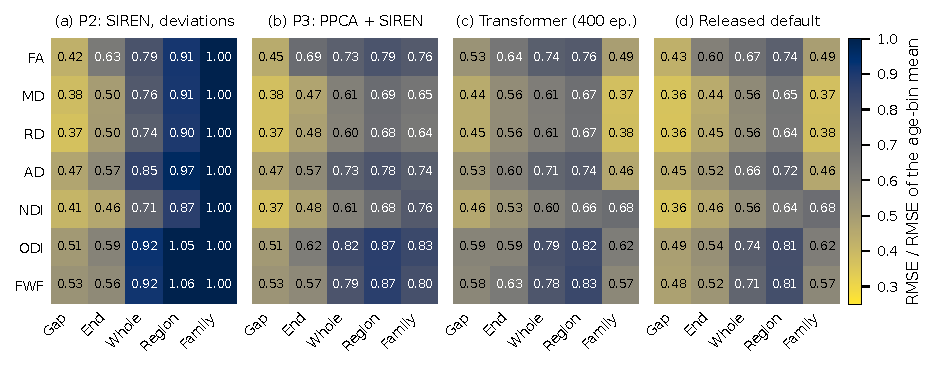
\includegraphics[width=\textwidth]{figures/fig_metric_heat.pdf}
\caption{Error relative to the age-bin mean per measure and pattern (mean over age bins and 3 seeds) for four settings.
``Family'': the measure's family hidden (1.00 for the norm-referenced SIREN, which cannot impute it).}\label{fig:metricheat}
\end{figure}

\paragraph{Measures.} MD, RD and NDI were imputed best (released default \mMDFinal, \mRDFinal{} and \mNDIFinal{}); FA,
AD, ODI and FWF worst (\mFAFinal, \mADFinal, \mODIFinal, \mFWFFinal; Appendix Table~\ref{tab:metric}, Fig.~\ref{fig:metricheat}).
For a missing family the tensor measures were recovered well from NODDI (MD \mMDWmFinal, FA \mFAWmFinal), the NODDI
measures less well from the tensor (NDI \mNDIWmFinal, ODI \mODIWmFinal, FWF \mFWFWmFinal).

\paragraph{Age.} Relative to the age-bin mean the error varied little with age (Fig.~\ref{fig:age}a, b; PPCA + SIREN
\rDefaultBinA, \rDefaultBinB{} and \rDefaultBinC{} in the three bins); the ranking of the methods was the same in every
age group, and the youngest and oldest groups have wide intervals (few scans). In absolute terms the age-bin mean's
diffusivity errors were largest at 0--3 months, and the released default halved them (Appendix Table~\ref{tab:absolute},
Fig.~\ref{fig:age}c).

\begin{figure}[t]
\centering
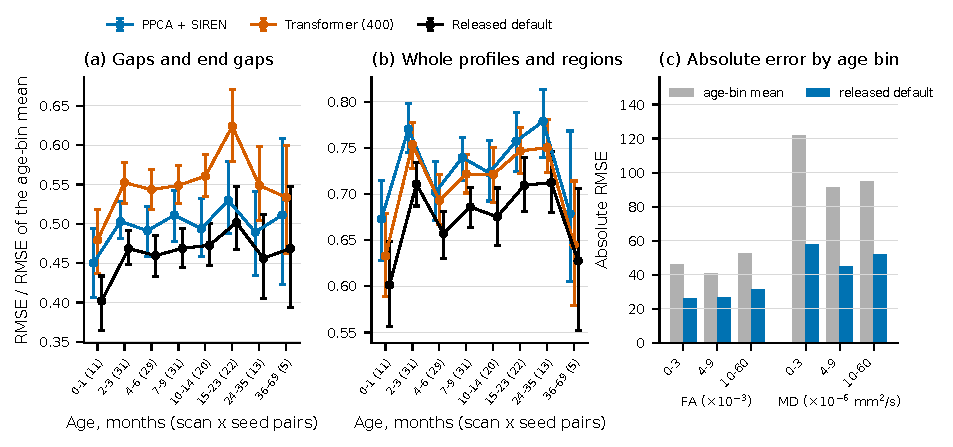
\includegraphics[width=\textwidth]{figures/fig_age.pdf}
\caption{Error by age. (a, b) Error relative to the age-bin mean per age group (cell dumps, 3 seeds; error bars: 95\%
bootstrap CI over scan $\times$ seed pairs, their number in parentheses) for PPCA + SIREN, the transformer alone and
the released default. (c) Absolute RMSE of FA and MD of the age-bin mean and the released default per age bin.}\label{fig:age}
\end{figure}

\paragraph{Tracts.} The whole-profile error of the released default ranged from \trBest{} (\trBestName) to \trWorst{}
(\trWorstName) across tracts (Fig.~\ref{fig:tracts}); \trAboveEight{} tracts were above 0.8 and none above 1. Tracts far
from other tracts were imputed worse (Spearman \trRhoProx, $p=$~\trRhoProxP); tract length did not matter.

\begin{figure}[t]
\centering
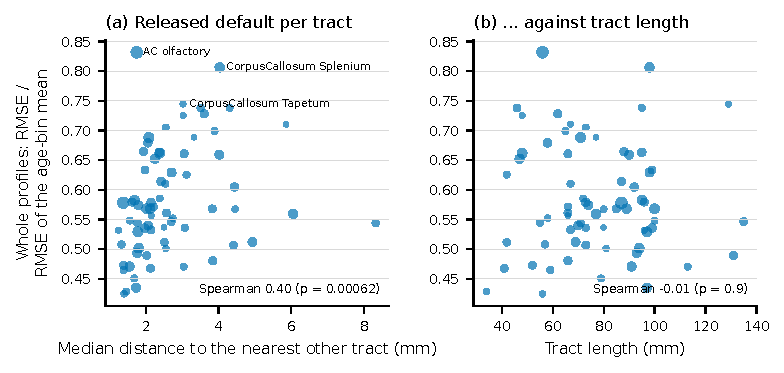
\includegraphics[width=0.85\textwidth]{figures/fig_tracts.pdf}
\caption{Whole-profile error of the released default per tract (seeds 0--2) against (a) the median distance to the
nearest other tract and (b) the tract length; marker area $\propto$ the tract's real rejection rate.}\label{fig:tracts}
\end{figure}

\subsection{Uncertainty}

The SD that \texttt{impute-profiles} writes for a blended value combines the PPCA and transformer SDs with the blend
weights. For the released default (Appendix Tables~\ref{tab:calib} and \ref{tab:calibband}), the root-mean-square of
error/SD was \calFinalWholeRms{} for whole profiles and \calFinalRegionRms{} for regions (\calFinalWholeCov\% and
\calFinalRegionCov\% of errors within 1.96 SD), \calFinalFamilyRms{} for a missing family (slightly too small SDs), and
\calFinalNearRms{} within 0.5\,mm of an observed value (SDs about twice too large: the PPCA SD is an upper bound for
locally imputed values); beyond 4\,mm it was \calFinalFarRms. The HBCD-reference blend was better calibrated for a missing
family (\calRefFamilyRms). Users can treat the SDs as conservative near observed values and as about right elsewhere;
a per-band rescaling is in Appendix Table~\ref{tab:calibband}.

\subsection{Downstream analyses}\label{sec:e4}

Table~\ref{tab:e4} and Fig.~\ref{fig:e4} summarise \efMainReps{} replicates per scenario. With the real prevalence of
missing values, complete-case analysis kept \efMainCcN{} of the 220 scans: its trajectory CIs were \efMainCcCi{} times as
wide as with complete data, its curves deviated more from the complete-data curves (\efMainCcBias{} SD; with random
masks this is the sampling deviation of a fit on half the scans, not a bias) and, for a
planted effect of 0.1 SD, its power fell from \efSmallFullPower\% to \efSmallCcPower\%. Every imputer kept all scans and
reproduced the complete-data analysis closely: trajectory deviation \efMainBlendBias{} SD (age-bin mean \efMainMeanBias),
CI width \efMainBlendCi{}, coverage \efMainBlendCoverage\%, power \efMainBlendPower\% for $\delta = 0.3$ and
\efSmallBlendPower\% for $\delta = 0.1$, type I error \efMainBlendTypei\% (cluster-robust SEs with 133 subjects are slightly liberal for every
imputer, complete-case analysis included).
Imputation attenuated a planted group effect only slightly (estimate \efMainBlendRelfull{} of the complete-data estimate
for the blend, \efMainPpcaRelfull{} for PPCA, \efMainMeanRelfull{} for the age-bin mean; difference \efMainBlendDiffsd{} SD),
because only a few percent of each tract's values were missing (\efMainMissShare\%). At $\delta = 0.1$ the ratio of
estimates is a ratio of small, noisy numbers (complete case \efSmallCcRelfull); the differences in SD units
(Table~\ref{tab:e4}) are the more reliable summary. When every scan carried a real mask, the age-bin mean attenuated the effect more
(\efSmallMissMeanRelfull) than PPCA (\efSmallMissPpcaRelfull) or the blend (\efSmallMissBlendRelfull), and complete-case
analysis was impossible. Multiple imputation from the PPCA posterior gave the same estimates and SEs as point imputation
(SE ratio \efMainMiSeratio): at this level of missingness, the between-imputation variance is negligible. Tract-wise
available-case analysis was nearly as good as imputation for single-tract analyses but cannot serve analyses of all
tracts jointly.

These scenarios assign the masks independently of group and values. In two further scenarios with differential
missingness, every scan of the group carrying the planted effect received a real mask and no scan of the other group
(about twice the cohort-wide share of imputed values in that group, \efDiffMissShare\% of each tract's values overall).
Complete-case analysis then removed the whole effect group and could not estimate the group effect. Every imputer
attenuated the effect by about the share of imputed values in the effect group: estimate \efDiffBlendRelfull{} of the
complete-data estimate for the blend, \efDiffPpcaRelfull{} for PPCA and \efDiffMeanRelfull{} for the age-bin mean at
$\delta = 0.3$ (difference \efDiffBlendDiffsd{} SD), with unchanged power (\efDiffBlendPower\%) and type I error
(\efDiffBlendTypei\%). Because the effect was planted in whole tracts, the imputed values carry no information about it,
and no imputer recovered it: imputation toward the norm shrinks a group difference in proportion to the imputed share of
the affected group. At the missingness of these cohorts the shrinkage is a few percent; it grows with that share.

\begin{table}[t]
\centering\footnotesize
\caption{E4: downstream analyses on 220 complete BCP scans with real masks transplanted (50 replicates per
scenario). Trajectory: FA and MD tract means $\sim$ spline(log age) on the tracts without a planted effect, against the
complete-data fit; deviation: mean absolute difference from the complete-data curve (SD of the tract mean). Group effect:
planted in 5 tracts; Est.\,$-$\,full: mean difference from the complete-data estimate (between-scan SD); type I: rejections
in the tracts without a planted effect. ``Group 1 masked'': differential missingness, masks only in the group with the
planted effect.}\label{tab:e4}
\resizebox{\textwidth}{!}{\begin{tabular}{llcccccccc}
\toprule
 & & \multicolumn{3}{c}{Trajectories (no effect planted)} & & \multicolumn{4}{c}{Planted group effect} \\
\cmidrule(lr){3-5}\cmidrule(lr){7-10}
Scenario & Imputer & Deviation (SD) & CI width & Coverage & Type I & Est.\,$-$\,full (SD) & Est.\,/\,full & SE / full & Power \\
\midrule
$\delta=0.3$, prevalence & complete case & 0.047 & 1.33 & 99\% & 5.6\% & +0.001 & 1.008 & 1.26 & 94\% \\
 & available case & 0.006 & 1.01 & 100\% & 5.3\% & +0.000 & 1.001 & 1.01 & 98\% \\
 & age-bin mean & 0.010 & 1.00 & 100\% & 5.1\% & -0.006 & 0.982 & 0.99 & 98\% \\
 & PPCA & 0.003 & 1.00 & 100\% & 5.6\% & -0.006 & 0.980 & 1.00 & 98\% \\
 & PPCA + kNN & 0.003 & 1.00 & 100\% & 5.6\% & -0.006 & 0.981 & 1.00 & 98\% \\
 & blend (table) & 0.003 & 1.00 & 100\% & 5.6\% & -0.006 & 0.980 & 1.00 & 98\% \\
 & multiple imputation (PPCA) & 0.003 & 1.00 & 100\% & 5.5\% & -0.006 & 0.980 & 1.00 & 98\% \\
\addlinespace[2pt]
$\delta=0.1$, prevalence & complete case & 0.047 & 1.33 & 99\% & 5.6\% & +0.001 & 1.177 & 1.26 & 26\% \\
 & available case & 0.006 & 1.01 & 100\% & 5.3\% & +0.000 & 1.045 & 1.01 & 37\% \\
 & age-bin mean & 0.010 & 1.00 & 100\% & 5.1\% & -0.002 & 1.007 & 0.99 & 36\% \\
 & PPCA & 0.003 & 1.00 & 100\% & 5.6\% & -0.002 & 0.982 & 1.00 & 34\% \\
 & PPCA + kNN & 0.003 & 1.00 & 100\% & 5.5\% & -0.002 & 0.975 & 1.00 & 35\% \\
 & blend (table) & 0.003 & 1.00 & 100\% & 5.5\% & -0.002 & 0.982 & 1.00 & 35\% \\
 & multiple imputation (PPCA) & 0.003 & 1.00 & 100\% & 5.6\% & -0.002 & 0.985 & 1.00 & 34\% \\
\addlinespace[2pt]
$\delta=0.1$, all masked & complete case & \multicolumn{8}{c}{every scan excluded} \\
 & available case & 0.010 & 1.02 & 100\% & 5.4\% & -0.000 & 1.043 & 1.01 & 35\% \\
 & age-bin mean & 0.020 & 1.00 & 100\% & 5.4\% & -0.005 & 0.938 & 0.99 & 35\% \\
 & PPCA & 0.005 & 0.99 & 100\% & 5.5\% & -0.004 & 0.993 & 0.99 & 34\% \\
 & PPCA + kNN & 0.005 & 1.00 & 100\% & 5.5\% & -0.004 & 0.994 & 0.99 & 33\% \\
 & blend (table) & 0.005 & 0.99 & 100\% & 5.5\% & -0.004 & 0.991 & 0.99 & 34\% \\
 & multiple imputation (PPCA) & 0.005 & 0.99 & 100\% & 5.4\% & -0.004 & 0.991 & 0.99 & 34\% \\
\addlinespace[2pt]
$\delta=0.3$, group 1 masked & complete case & 0.058 & 1.41 & 98\% & -- & -- & -- & -- & -- \\
 & available case & 0.006 & 1.01 & 100\% & 5.5\% & -0.000 & 1.000 & 1.01 & 98\% \\
 & age-bin mean & 0.011 & 1.00 & 100\% & 5.6\% & -0.012 & 0.959 & 1.00 & 98\% \\
 & PPCA & 0.003 & 1.00 & 100\% & 5.5\% & -0.013 & 0.956 & 1.00 & 98\% \\
 & PPCA + kNN & 0.003 & 1.00 & 100\% & 5.6\% & -0.012 & 0.957 & 1.00 & 98\% \\
 & blend (table) & 0.003 & 1.00 & 100\% & 5.7\% & -0.012 & 0.956 & 1.00 & 98\% \\
 & multiple imputation (PPCA) & 0.003 & 1.00 & 100\% & 5.5\% & -0.013 & 0.956 & 1.00 & 98\% \\
\addlinespace[2pt]
$\delta=0.1$, group 1 masked & complete case & 0.058 & 1.41 & 98\% & -- & -- & -- & -- & -- \\
 & available case & 0.006 & 1.01 & 100\% & 5.5\% & -0.000 & 1.025 & 1.01 & 36\% \\
 & age-bin mean & 0.011 & 1.00 & 100\% & 5.6\% & -0.003 & 0.997 & 1.00 & 35\% \\
 & PPCA & 0.003 & 1.00 & 100\% & 5.5\% & -0.004 & 0.975 & 1.00 & 34\% \\
 & PPCA + kNN & 0.003 & 1.00 & 100\% & 5.6\% & -0.004 & 0.987 & 1.00 & 33\% \\
 & blend (table) & 0.003 & 1.00 & 100\% & 5.6\% & -0.004 & 0.980 & 1.00 & 34\% \\
 & multiple imputation (PPCA) & 0.003 & 1.00 & 100\% & 5.5\% & -0.004 & 0.973 & 1.00 & 34\% \\
\bottomrule
\end{tabular}
}
\end{table}

\subsection{Statistical summary}

Appendix Table~\ref{tab:paired} and Appendix Fig.~\ref{fig:paired} collect the selected four-pattern contrasts. Under the subject-level
bootstrap, the CIs were nearly identical to the per-pair CIs. Differences of 1--2\% (components, blend weights, epochs)
were detectable because all settings saw the same hidden values; their practical relevance is small, and they were
selected on the same draws.

\section{Discussion}

\subsection{Principal findings}

\begin{enumerate}
\item \emph{A scan's own neighbouring tracts do not predict a missing tract.} Same-scan interpolation is useful only along
a profile.
\item \emph{The normative reference is the main source of information.} Imputing deviations from an age-appropriate
norm made every pattern imputable; a linear population model of how deviations co-vary across tracts and measures
improved whole profiles and regions further and made a missing measure family imputable.
\item \emph{The best local refinement depends on the pattern.} For whole missing tracts, the dominant real pattern, $k$NN
on the population residuals is better than SIREN; SIREN wins for gaps.
\item \emph{Amortized networks add most where local information is scarce}, beyond a few millimetres and for a
missing family, when they correct the population model and are blended with it.
\item \emph{A second cohort helps as training data for the transformer, not inside the population model.} Training the
transformer on both cohorts reduced its error (\pbDAll{} at equal epochs). Pooling the norm was harmless, but pooling the
PPCA multiplied the error by \eFiveB{} on the synthetic patterns and by \eFiveRealB{} on the real masks, with either age
norm. The different age scales (BCP chronological, HBCD term-corrected), acquisitions and preprocessing pipelines of the
cohorts are plausible reasons why their covariance structures differ.
\item \emph{The gains hold on untouched subjects and real masks.} On subjects never used for any design decision, the
released default had \eOneFinalVsDef{} of PPCA + SIREN's error (development: \cORatio), with the same ranking for whole
profiles and for the real missingness masks. On a second cohort (HBCD alone) the blend's gain was larger
(\eThreeFinalVsDef). With a large training cohort the transformer alone matched or beat the blend with the shipped BCP weights for
regions and real masks, but not for whole profiles, and a weight table refitted on the target cohort matched or beat it
everywhere. The population model gained little on HBCD's real masks (\rmThreeDefIn{} within the tool's scope, cell-weighted; per
scan \rmThreeScanInDef, better than the norm in only \rmThreeScanInDefBetter\% of scans against
\rmThreeScanInTfBetter\% for the transformer), was above the norm's cell-weighted error for the smallest masks
(\rmThreeShareADef) through a minority of poorly imputed scans, and was clearly worse than the norm when most of a scan
was hidden; for a large multi-site cohort the transformer is the safer choice.
\item \emph{At realistic missingness, imputation preserves typical analyses and complete-case analysis does not.}
With masks independent of group and values, imputation kept all scans with negligible bias and attenuation; complete-case
analysis lost about half of the scans, and its power for a 0.1-SD group effect fell from \efSmallFullPower\% to
\efSmallCcPower\%. With all masks in the group carrying the effect, every imputer attenuated the group effect by about the
imputed share of that group (\efDiffBlendRelfull{} of the complete-data estimate), without inflating type I error.
Multiple imputation was not needed at this level of missingness.
\end{enumerate}

\subsection{Interpretation}

The PPCA posterior is the exact conditional expectation under a Gaussian model with one loading per cell; with 80
components it captures the main covariation of 37,716 cells from a few hundred scans. Functa and the partial VAE
replace this exact inference by a latent fitted with a few gradient steps or an encoder, and with hundreds of scans they
did not learn a better prior. The networks that read each location's observed value directly and only learn a
correction to the PPCA prediction were better, most where PPCA has least local information. We offer some hypotheses
that our data do not test: that neighbouring tracts differ systematically by their orientation and organization (which
would explain the failure of same-scan methods), that the transformer's global attention explains its advantage over the U-Net (the training budget does not, O5), and that context inputs did not help because the observed values already
encode age and acquisition.

\subsection{Limitations}

\begin{itemize}
\item \emph{One normative cohort for development.} Choices were made on seeds 0--2; E1 tests them on untouched subjects
of 4--60 months only (the 0--3 month bin was exhausted), and E3 on a second cohort (with the transformer trained for 200 instead of 400 epochs).
\item \emph{Missingness mechanism.} The synthetic patterns hide values at random within each pattern; the real-mask pass
reproduces the real masks but not a possible dependence between rejection and the true values (missing not at random).
\item \emph{QC truncates the hidden values.} The profile QC removed tracts that deviated by more than 3.5 SD from a prior
built on the full BCP cohort, so only values that passed this outlier filter could be hidden. The errors are therefore
likely optimistic for atypical scans, such as those of clinical cohorts or with residual artefacts.
\item \emph{Reference of the score.} Ratios to the age-bin mean depend on how good that mean is; the kernel-norm
reference and absolute RMSEs (Table~\ref{tab:rev}, Appendix Table~\ref{tab:absall}) give the same ranking. BCP ages are
nominal whole months.
\item \emph{Age scales of the cohorts.} BCP ages are chronological, HBCD ages term-corrected. For infants born before term
the scales differ by $40-\text{GA}$ weeks, so pooled norms, the batch correction and the 0--3 month results compare
slightly different developmental ages. This plausibly contributes to the residual cohort difference at 1.5--3.5 months and
to the age dependence of pooling, but gestational age is not in our data and we could not test it. Correcting both cohorts
to a common age scale (e.g.\ postmenstrual age) before pooling is left for future work. The cohorts were also acquired differently and preprocessed with different pipelines (\path{dmriprep}, QSIPrep;
the model fitting and later steps were the same), which may add cohort differences beyond a shift and scale per cell.
\item \emph{NODDI in infants.} NODDI was fitted with AMICO's default (adult) intrinsic diffusivities, which differ from
those of the infant brain \citep{cieslak2025hbcd}; NDI, ODI and FWF are therefore model-dependent indices whose absolute
values should be interpreted with care, although this does not affect the comparison of imputation methods.
\item \emph{Dependence and training variance.} The subject bootstrap handles repeated seeds and sessions but not the
variation from network training; some checks used one seed or one split.
\item \emph{Measures and atlas.} Seven measures of one atlas with dense tract axes; sparser tract sets give fewer close
neighbours.
\end{itemize}

\subsection{Practical recommendations}

\begin{enumerate}
\item \emph{Without a normative reference}, fill only gaps along a profile (arc-linear); do not impute whole tracts from
the scan's own neighbours.
\item \emph{With a normative cohort and whole missing tracts (the common case)}, fit a population
model (PPCA, about 80 components) of the deviations from an age-appropriate norm and refine it locally with $k$NN on its
residuals within 4\,mm; this needs no GPU. The error falls steadily with the size of the normative cohort, without a
threshold: relative to about \oNA{} scans, the whole-profile error was \oPairQKnn{} times as large with about \oNQ, \oPairHKnn{}
with about \oNH{} and \oPairTKnn{} with about \oNT{} (norm and PPCA refitted on each subset; Section~\ref{sec:o1o3}).
In a large multi-site cohort (HBCD) the population model gained little for spatially clustered missingness (regions
\eThreeKnnRegion, real masks \rmThreeKnnIn{} for PPCA + $k$NN), so a GPU-trained transformer is worth its cost there. Keep the three broad age bins: finer bins did not
help under the population model.
\item \emph{If short gaps along profiles matter}, use SIREN on the residuals instead (a combination of $k$NN for whole tracts and SIREN within 2\,mm for gaps is plausible
but was not evaluated).
\item \emph{With a GPU}, blend with a transformer trained to correct the population model, with weights growing with the
distance to the nearest observed value (the default of DTIPlayground 0.9.8); this is most valuable when whole measure
families are missing. With a large normative cohort (thousands of scans, as HBCD), the transformer alone matched or beat the blend with the shipped BCP
weights for regions and real masks, though not for whole profiles; a weight table refitted on the target cohort
(\path{--ensemble-weights fit}) matched or beat the transformer alone for every pattern, so refit the weights, or check
the blend against the transformer alone in a validation of the target cohort.
\item \emph{With a second cohort on the same tracts}, use it to train the transformer, and keep the population model
of the target cohort; the norm can be pooled after a batch correction (it neither helped nor hurt overall, \eFiveA, and helped
slightly in the thin 0--3 month bin, 0.977 [0.955, 0.999]; E5, Table~\ref{tab:e5}), preferably after bringing both cohorts to a common age scale (chronological vs
term-corrected or postmenstrual age).
\item \emph{Report and check}: report the share of imputed values, per group, keep the masks and SDs, and check that
conclusions hold without imputed values. At the levels of missingness seen in BCP and with missingness unrelated to
group, point imputation preserved trajectory and group analyses and was much better than complete-case analysis. When
one group has more rejected tracts (a clinical or high-motion group), imputation toward the norm shrinks the group
difference by about the imputed share of that group: compare group results with tract-wise available-case analysis, and
do not rely on imputed values for group differences between normative and clinical scans, whose deviations the norm of a
typically developing cohort does not represent. With much more missingness, prefer the population model or the blend
over the age-bin mean (less attenuation when every scan is masked) and consider multiple imputation from the PPCA
posterior.
\end{enumerate}

\section{Conclusion}

In a developmental cohort with dense atlas tracts, missing diffusion profile values are best imputed as deviations from
an age-appropriate norm, using a joint population model of all tracts and measures, refined locally near observed values
and, with a GPU, blended with a transformer trained to correct it. Several more complex alternatives did not help.
The gains reproduced on untouched subjects and real missingness masks, and at the missingness of a typical infant
cohort imputation preserved downstream analyses that complete-case analysis would weaken; with missingness concentrated in
one group it shrinks that group's difference by about its imputed share. On a second, larger infant cohort, the ranking
transferred, the amortized transformer gained most, and blend weights refitted on that cohort did best. All methods, the validation protocol and the defaults are available in DTIPlayground.

\section*{Data and code availability}

DTIPlayground (including \path{dmrifiberprofile impute-profiles} and its \path{--validate} protocol) is open source
at \url{https://github.com/NIRALUser/DTIPlayground}, on PyPI (\texttt{dtiplayground}; this paper: version 0.9.9, GitHub tag v0.9.9) and on Docker Hub
(\texttt{niraluser/dtiplayground:0.9.9}) \todo{Zenodo DOI of the release}. The processing scripts (model fitting, registration, registration QC, profile extraction and profile QC) and the
\path{dmriprep} protocol will be shared with the paper \todo{author: where}. The scripts that compute every number, table and figure from the
validation result files, together with the manuscript sources, are in the same repository under
\path{papers/ProfileImputation} (\path{scripts/run_all.sh}); the validation
result files (per-scan, per-age-bin and per-distance tables and the per-cell dumps) will be released \todo{repository and
DOI}. BCP data are publicly available through the NIMH Data Archive (NDA) \todo{author: NDA collection ID, if cited}; the profiles
used here were processed by the BCP imaging core from the study's imaging data; HBCD data (release v2.0) are available through the NIH Brain Development Cohorts (NBDC) Data Sharing Platform
\todo{author: DUA or study number, if required}. \todo{Whether
derived profile tables can be shared.}

\section*{Acknowledgements}
This work was supported by NIH grants U01-MH110274 (W.L., J.T.E., M.A.S.), R01-MH104324 and P50-HD103573 (J.T.E.,
M.A.S.), R01-MH123747, R01-MH070890, R01-HD053000 and R01-MH064065 (J.H.G.), and R01-HD055741 and R01-MH118362
(M.A.S.), and by the efforts of the UNC/UMN Baby Connectome Project Consortium.

Data used in the preparation of this article were obtained from the HEALthy Brain and Child Development (HBCD) Study,
held in the NIH Brain Development Cohorts Data Sharing Platform. This is a multisite, longitudinal study designed to
recruit approximately 7,000 families and follow them from pregnancy to early childhood. The HBCD Study is supported by
the NIH and additional federal partners under award numbers U01DA055352, U01DA055353, U01DA055366, U01DA055365,
U01DA055362, U01DA055342, U01DA055360, U01DA055350, U01DA055338, U01DA055355, U01DA055363, U01DA055349, U01DA055361,
U01DA055316, U01DA055344, U01DA055322, U01DA055369, U01DA055358, U01DA055371, U01DA055359, U01DA055354, U01DA055370,
U01DA055347, U01DA055357, U01DA055367, U24DA055325, and U24DA055330. A full list of supporters is available at
\url{https://hbcdstudy.org/federal-partners/}. A full list of participating sites is available at
\url{https://hbcdstudy.org/study-sites/}. HBCD Study Consortium investigators designed and implemented the study and/or
provided data but did not necessarily participate in the analysis or writing of this report. This manuscript reflects
the views of the authors and may not reflect the opinions or views of the NIH or the HBCD Study Consortium
investigators.

\section*{Author contributions}
\todo{CRediT statement.}

\section*{Declaration of competing interests}
\todo{Competing interests.}

\bibliographystyle{plainnat}
\bibliography{refs}

\clearpage
\appendix
\section{Supplementary material}
\setcounter{figure}{0}\renewcommand{\thefigure}{A\arabic{figure}}
\setcounter{table}{0}\renewcommand{\thetable}{A\arabic{table}}

\subsection{Acquisition, preprocessing and processing}\label{sec:procdetail}

\paragraph{BCP.} The BCP is a joint study of the University of North Carolina at Chapel Hill and the University of Minnesota that enrols
typically developing children between birth and 5 years of age in a hybrid accelerated longitudinal and cross-sectional
design (planned: 500 children, 285 of them with 4--6 longitudinal visits) \citep{howell2019bcp}. Children were eligible
if born at 37--42 weeks of gestation with a birth weight appropriate for gestational age and without major pregnancy and
delivery complications; exclusion criteria included a first-degree relative with autism, intellectual disability,
schizophrenia or bipolar disorder, significant medical or genetic conditions affecting growth, development or
cognition, and contraindications to MRI \citep{howell2019bcp}. Children were scanned without sedation, the younger ones
during natural sleep, on 3T Siemens Prisma scanners with 32-channel head coils at both sites. The diffusion protocol of
\citet{howell2019bcp} is a 6-shell scheme ($b$ = 500, 1000, 1500, 2000, 2500 and 3000\,s/mm$^2$ with 9, 12, 17, 24, 34
and 48 directions, 6 $b=0$ images), acquired at 1.5\,mm isotropic resolution with multiband factor 5 in both the AP and
PA phase-encoding directions (6:58 each); in children who stayed asleep, a 2-shell scheme with 79 directions ($b$ = 1500
and 3000\,s/mm$^2$, multiband factor 4, 1.5\,mm isotropic, AP and PA, 4:35 each) was added, and was prioritized for
longitudinal participants of an earlier study to keep their data compatible. Parents provided permission and informed
consent, and the procedures were approved by the Institutional Review Boards of both universities
\citep{howell2019bcp}. The labels of the scans give the sequence: \texttt{\bcpAcqAName} (\bcpAcqAN{} scans) the 79-direction 2-shell sequence,
\texttt{\bcpAcqBName} (\bcpAcqBN{}) and \texttt{\bcpAcqCName} (\bcpAcqCN{}) the 6-shell sequence (by age bin in Appendix
Table~\ref{tab:acq}). Some sessions have only one sequence, others both; a session with both contributes two scans, each
processed and profiled separately (\bcpSessionsBoth{} of \bcpSessions{} sessions). The BCP scans were preprocessed with
\path{dmriprep} of DTIPlayground (version 0.5.7; \citealp{dtiplayground}) with a protocol of five modules: a slice-wise
intensity check and an interlace (inter-slice correlation and motion) check that exclude corrupted gradient volumes, as
in DTIPrep \citep{oguz2014dtiprep}; susceptibility-distortion correction with FSL's topup from the reverse
phase-encoded acquisitions \citep{andersson2003topup}; eddy-current and head-motion correction with FSL's eddy, with
susceptibility-by-movement estimation and replacement of outlier slices \citep{andersson2016eddy}; and a weighted
least-squares tensor fit; a QC report lists the excluded gradients and the motion of every scan. The BCP data were processed by the BCP imaging
core (UNC) from the study's own imaging data.

\paragraph{HBCD.} HBCD scans were acquired at multiple sites on Siemens, GE and Philips scanners with two complete
multi-shell acquisitions of opposite phase-encoding direction (AP and PA), each with $b$ = 0, 500, 1000, 2000 and
3000\,s/mm$^2$ (10, 6, 12, 18 and 30 volumes), 87 contiguous 1.7-mm axial slices with a $140\times140$ matrix and a 238-mm field of view, multiband factor 3, TR 4800\,ms and TE 88\,ms
\citep{dean2024hbcdmri,cieslak2025hbcd}. They were preprocessed with QSIPrep as described by \citet{cieslak2025hbcd}:
partial-Fourier Gibbs unringing, MP-PCA denoising, susceptibility-distortion, eddy-current and head-motion correction
with FSL's topup and eddy followed by a second distortion correction with DRBUDDI (TORTOISE), brain extraction with
SynthStrip on the T2-weighted image, and resampling to an AC-PC space aligned with the T2-weighted image. The derived
maps of QSIRecon were not used; the diffusion models were fitted to the QSIPrep outputs as described below.

\paragraph{Processing.} Both cohorts then went through the same steps. (i)~\emph{Models.} Within the brain mask (for HBCD that of QSIPrep), the diffusion tensor was fitted by weighted
least squares with DIPY \citep{garyfallidis2014dipy} on the volumes with $b \le 1600$\,s/mm$^2$: for HBCD the shells
of 500 and 1000\,s/mm$^2$, for the BCP 6-shell sequence those of 500 to 1500\,s/mm$^2$ and for the 79-direction sequence
the shell of 1500\,s/mm$^2$; NODDI
\citep{zhang2012noddi} was fitted with AMICO \citep{daducci2015amico} on all shells, with AMICO's default model
settings (no infant-specific intrinsic diffusivities were set; 2000 kernel orientations); and the free-water corrected
tensor \citep{pasternak2009freewater,hoy2014fwdti} with DIPY (non-linear least squares, all shells), whose measures were
not used here. (ii)~\emph{Registration.} Each tensor image was registered with the DTI\_Register module of
\path{dmriprep} (DTI-Reg; \citealp{verde2014unc}): an affine registration of the FA images (BRAINSFit) refined by a
greedy diffeomorphic ANTs registration with a cross-correlation metric \citep{avants2008syn}, the tensors resampled
log-Euclidean with reorientation \citep{arsigny2006logeuclidean}, to the age-appropriate mean tensor of a normative model
of the pediatric DTI\_IBISEP\_Feb26 atlas (one mean tensor per age bin, on the atlas grid), after an automatic check and
correction of the tensor frame. The atlas was built from IBIS data starting from the UNC pediatric atlas
\citep{short2022atlas}; its normative model (mean tensors and their spread per age bin), used for the registration and the registration QC, and
the prior age-bin profile statistics used in the profile QC were built with DTIPlayground from the full BCP cohort. These
full-cohort statistics enter only the processing and QC stage, which defined the real missingness, and the norm of the
released imputation default; the validation does not use them: in every validation run the age-bin norm, the
population models and the networks were refitted from the cohort itself without the validated subjects (leave-subject-out
folds; no validation setting used the precomputed statistics). (iii)~\emph{Registration QC.} \path{dmrifiberprofile
qc-registration} compared each registered scan with the atlas and the age-binned normative model (FA and the
diffusivities: mean absolute error, structural similarity, correlation, principal-direction angular error, contiguity of the disagreement,
and a check of the ventricles) and flagged a session as a registration failure by a robust Mahalanobis distance over these
features. (iv)~\emph{Profiles.} Profiles were extracted with the EXTRACT\_Profile module of \path{dmrifiberprofile}
in each scan's native space: the arc-length-parametrized fibers of each atlas tract were mapped into the scan through
its deformation field, so that the tensors did not need to be resampled into atlas space; FA, MD, RD and AD were computed
from the tensors interpolated log-Euclidean along the fibers, NDI, ODI and FWF sampled from their maps. The profile was
sampled every 1\,mm of the stored atlas arc length, from an origin at the tract's median plane, so that all scans share the
atlas's sampling grid, and points within a Gaussian kernel of 3\,mm SD around each sample were averaged.
The profile QC that follows is described in Section~\ref{sec:data}.

\subsection{Supplementary tables and figures}


\begin{table}[h]
\centering\footnotesize
\caption{Development history: the phases in which the methods were added to DTIPlayground, and where they appear
here.}\label{tab:phases}
\begin{tabular}{lp{9.5cm}p{3.2cm}}
\toprule
Phase (release) & Methods & Family here \\
\midrule
1 & arc-linear, linear, $k$NN, SIREN on the scan's own values & A \\
2 (0.8.20) & the same on deviations from the age-bin norm & B \\
3 (0.8.21) & PPCA, PPCA + $k$NN / SIREN (default up to 0.9.5) & C \\
3b (0.8.22) & continuous age norms, pooling with batch correction & C, second cohort \\
4 (0.8.23) & graph U-Net after CONFETTI & E \\
5 & functa (not adopted) & G \\
6 (0.9.8) & transformer, partial VAE, age-dependent PPCA, acquisition correction, blends & E, F, G \\
revision & generic cohort imputers, untouched test, real masks, HBCD, downstream & D, Sections 4.5--4.10 \\
\bottomrule
\end{tabular}
\end{table}

\begin{table}[h]
\centering\footnotesize
\caption{Generic cohort imputers (E8) on the hidden values of seeds 0--2 (same training scans per fold as PPCA), with
the paired whole-profile ratio against PPCA alone (95\% subject-bootstrap CI).}\label{tab:baselines}
\resizebox{\textwidth}{!}{\begin{tabular}{lcccccccc}
\toprule
Setting & Overall (SD) & Gap & End & Whole & Region & Tensor & NODDI & Whole: paired vs PPCA \\
\midrule
offset (measure) & 0.903 (0.011) & 0.870 & 0.939 & 0.887 & 0.917 & 1.002 & 1.000 & 1.218 [1.194, 1.244] \\
offset (5 tracts) & 0.898 (0.007) & 0.853 & 0.927 & 0.876 & 0.936 & 1.002 & 1.000 & 1.202 [1.181, 1.226] \\
kNN across scans, k=5 & 0.856 (0.011) & 0.822 & 0.898 & 0.838 & 0.867 & 0.819 & 0.936 & 1.167 [1.150, 1.185] \\
kNN across scans, k=10 & 0.838 (0.009) & 0.811 & 0.877 & 0.821 & 0.843 & 0.803 & 0.914 & 1.140 [1.125, 1.157] \\
kNN across scans, k=20 & 0.837 (0.011) & 0.811 & 0.872 & 0.821 & 0.842 & 0.802 & 0.910 & 1.134 [1.118, 1.151] \\
kNN across scans, k=50 & 0.854 (0.010) & 0.829 & 0.886 & 0.839 & 0.862 & 0.830 & 0.918 & 1.152 [1.134, 1.171] \\
iterative SVD, rank 10 & 0.789 (0.014) & 0.758 & 0.839 & 0.773 & 0.786 & 0.768 & 0.857 & 1.083 [1.070, 1.097] \\
iterative SVD, rank 40 & 0.752 (0.012) & 0.716 & 0.798 & 0.732 & 0.764 & 0.721 & 0.810 & 1.023 [1.016, 1.031] \\
iterative SVD, rank 80 & 0.736 (0.008) & 0.688 & 0.781 & 0.715 & 0.758 & 0.698 & 0.800 & 1.001 [0.999, 1.003] \\
iterative SVD, rank 160 & 0.727 (0.007) & 0.669 & 0.760 & 0.709 & 0.769 & 0.674 & 0.786 & 0.990 [0.979, 1.000] \\
MICE (tract means) & 0.843 (0.016) & 0.813 & 0.906 & 0.820 & 0.831 & 0.868 & 0.910 & 1.146 [1.128, 1.165] \\
\midrule
PPCA alone & 0.733 (0.008) & 0.685 & 0.777 & 0.713 & 0.759 & 0.696 & 0.798 & -- \\
PPCA + kNN & 0.664 (0.008) & 0.568 & 0.659 & 0.675 & 0.752 & 0.696 & 0.798 & -- \\
PPCA + SIREN & 0.614 (0.007) & 0.440 & 0.552 & 0.697 & 0.766 & 0.696 & 0.798 & -- \\
\bottomrule
\end{tabular}
}
\end{table}

\begin{table}[h]
\centering\footnotesize
\caption{Distance limit of the local methods under the current protocol: the local method fills cells up to the limit,
PPCA beyond (normalized squared errors of the same cells pooled over age bins, relative to the age-bin mean; mean over
measures).}\label{tab:cap}
\begin{tabular}{llccccc}
\toprule
Local method & Limit & Gap & End & Whole & Region & Overall \\
\midrule
SIREN & PPCA only & 0.652 & 0.754 & 0.688 & 0.728 & 0.706 \\
 & 2 mm & 0.486 & 0.605 & 0.659 & 0.722 & 0.618 \\
 & 4 mm & 0.416 & 0.539 & 0.665 & 0.731 & 0.588 \\
kNN & PPCA only & 0.652 & 0.754 & 0.688 & 0.728 & 0.706 \\
 & 2 mm & 0.558 & 0.655 & 0.649 & 0.718 & 0.645 \\
 & 4 mm & 0.532 & 0.634 & 0.637 & 0.717 & 0.630 \\
\bottomrule
\end{tabular}

\end{table}

\begin{table}[h]
\centering\footnotesize
\caption{Absolute RMSE of the main settings (four patterns; mean over patterns, age bins and seeds); FA, NDI, ODI, FWF
$\times10^{3}$, MD, RD, AD $\times10^{6}$\,mm$^2$/s.}\label{tab:absall}
\begin{tabular}{lccccccc}
\toprule
Setting & FA & MD & RD & AD & NDI & ODI & FWF \\
\midrule
Age-bin mean & 46.3 & 102.6 & 101.6 & 125.8 & 65.5 & 51.8 & 56.2 \\
Kernel age norm (alone) & 40.7 & 90.4 & 86.4 & 120.1 & 57.3 & 50.4 & 55.3 \\
Phase 2: SIREN on deviations & 31.5 & 64.9 & 63.0 & 89.7 & 40.1 & 38.7 & 43.5 \\
PPCA alone & 36.1 & 67.2 & 65.7 & 95.1 & 43.2 & 41.9 & 45.7 \\
PPCA + kNN & 32.2 & 60.5 & 59.4 & 87.0 & 37.9 & 38.5 & 41.9 \\
PPCA + SIREN & 30.5 & 54.4 & 53.7 & 80.4 & 35.1 & 35.9 & 39.0 \\
Graph U-Net alone & 32.2 & 61.6 & 60.3 & 87.6 & 39.7 & 39.0 & 42.5 \\
Transformer alone (400) & 30.7 & 58.4 & 57.3 & 81.4 & 36.9 & 35.6 & 39.9 \\
Blend, fixed (400) & 28.3 & 51.7 & 50.9 & 75.1 & 33.3 & 33.3 & 36.4 \\
Released default (table) & 28.0 & 51.5 & 50.7 & 73.9 & 33.1 & 32.8 & 35.7 \\
HBCD-trained transformer, table & 26.5 & 48.8 & 47.8 & 70.3 & 31.6 & 30.8 & 33.5 \\
\bottomrule
\end{tabular}

\end{table}

\begin{table}[h]
\centering\footnotesize
\caption{Calibration of the predicted SDs: root-mean-square of error/SD (1: right; below 1: SDs too large) and share of
errors within 1.96 SD (95\%: right), mean over measures, seeds 0--2 (cell dumps).}\label{tab:calib}
\begin{tabular}{lccccc}
\toprule
Setting & Gap & End & Whole & Region & Family \\
\midrule
PPCA + SIREN & 0.59 / 99\% & 0.78 / 97\% & 0.93 / 96\% & 1.06 / 95\% & 1.06 / 95\% \\
Transformer (400) & 0.97 / 96\% & 1.02 / 96\% & 1.08 / 94\% & 1.08 / 94\% & 1.20 / 94\% \\
Released default (table) & 0.58 / 99\% & 0.72 / 98\% & 0.86 / 97\% & 0.96 / 96\% & 1.10 / 95\% \\
Table, shipped weights & 0.58 / 99\% & 0.72 / 98\% & 0.86 / 97\% & 0.96 / 96\% & 1.10 / 95\% \\
HBCD-reference table blend & 0.58 / 99\% & 0.68 / 98\% & 0.82 / 98\% & 0.89 / 97\% & 0.93 / 97\% \\
\bottomrule
\end{tabular}

\end{table}

\begin{table}[h]
\centering\footnotesize
\caption{Root-mean-square of error/SD per weight-table distance band (all patterns); dividing the written SDs by
these factors calibrates them.}\label{tab:calibband}
\resizebox{\textwidth}{!}{\begin{tabular}{lcccccccccc}
\toprule
Setting & 0-0.5 & 0.5-1 & 1-2 & 2-3 & 3-4 & 4-6 & 6-10 & 10-20 & $>$20 & none \\
\midrule
PPCA + SIREN & 0.59 & 0.61 & 0.77 & 0.94 & 1.06 & 1.04 & 1.10 & 1.06 & 1.21 & 1.06 \\
Transformer (400) & 1.01 & 0.99 & 1.02 & 1.04 & 1.06 & 1.10 & 1.12 & 1.09 & 1.14 & 1.20 \\
Released default (table) & 0.55 & 0.56 & 0.71 & 0.83 & 0.92 & 0.98 & 1.02 & 0.99 & 1.08 & 1.10 \\
HBCD-reference table blend & 0.53 & 0.56 & 0.70 & 0.80 & 0.87 & 0.90 & 0.93 & 0.91 & 0.96 & 0.93 \\
\bottomrule
\end{tabular}
}
\end{table}

\begin{table}[h]
\centering\footnotesize
\caption{Blend learners on the cell dumps, cross-fitted per seed (mean over seeds 0--2).}\label{tab:learners}
\resizebox{\textwidth}{!}{\begin{tabular}{llccccccc}
\toprule
Transformer & Blend & Overall & Gap & End & Whole & Region & Tensor & NODDI \\
\midrule
BCP transformer (400 ep.) & PPCA + SIREN & 0.614 & 0.440 & 0.552 & 0.697 & 0.766 & 0.696 & 0.798 \\
 & transformer alone & 0.632 & 0.510 & 0.588 & 0.694 & 0.737 & 0.425 & 0.623 \\
 & fixed 0.25/0.75 & 0.576 & 0.414 & 0.509 & 0.654 & 0.726 & 0.443 & 0.630 \\
 & weights per measure x distance (finer bands) & 0.569 & 0.418 & 0.506 & 0.639 & 0.715 & 0.425 & 0.623 \\
 & calibrated precision weights & 0.572 & 0.423 & 0.503 & 0.643 & 0.721 & 0.471 & 0.667 \\
 & gradient-boosted weight per cell & 0.569 & 0.418 & 0.504 & 0.638 & 0.715 & 0.425 & 0.624 \\
\addlinespace[2pt]
HBCD-reference transformer (200 ep.) & PPCA + SIREN & 0.614 & 0.440 & 0.552 & 0.697 & 0.766 & 0.696 & 0.798 \\
 & transformer alone & 0.580 & 0.456 & 0.532 & 0.633 & 0.698 & 0.432 & 0.662 \\
 & fixed 0.25/0.75 & 0.557 & 0.400 & 0.495 & 0.634 & 0.697 & 0.439 & 0.642 \\
 & weights per measure x distance (finer bands) & 0.541 & 0.398 & 0.481 & 0.604 & 0.680 & 0.429 & 0.646 \\
 & calibrated precision weights & 0.542 & 0.398 & 0.473 & 0.611 & 0.687 & 0.469 & 0.650 \\
 & gradient-boosted weight per cell & 0.538 & 0.398 & 0.474 & 0.602 & 0.678 & 0.431 & 0.637 \\
\bottomrule
\end{tabular}
}
\end{table}

\begin{table}[h]
\centering\footnotesize
\caption{Graph U-Net development (seed 0, 54 scans, 11 measures): from CONFETTI's configuration to the hybrid.}\label{tab:confetti}
\begin{tabular}{lcccccc}
\toprule
Setting (seed 0, 54 scans, 11 measures) & Overall & Gap & End & Whole & Region & Family \\
\midrule
CONFETTI configuration: fiber graph, 64 features & 0.899 & 0.882 & 0.894 & 0.899 & 0.920 & 0.673 \\
Fiber graph, 128 features & 0.877 & 0.855 & 0.874 & 0.877 & 0.903 & 0.644 \\
Axis graph, 128 features & 0.743 & 0.654 & 0.748 & 0.751 & 0.818 & 0.488 \\
Axis graph, 256 features & 0.729 & 0.625 & 0.748 & 0.738 & 0.806 & 0.464 \\
Hybrid (corrects PPCA), axis graph, 128 features & 0.635 & 0.563 & 0.638 & 0.638 & 0.701 & 0.438 \\
Hybrid, axis graph, 256 features, 2 convolutions & 0.623 & 0.543 & 0.620 & 0.632 & 0.699 & 0.432 \\
PPCA alone (same run) & 0.685 & 0.638 & 0.721 & 0.662 & 0.717 & 0.639 \\
PPCA + SIREN (same run) & 0.572 & 0.408 & 0.516 & 0.642 & 0.720 & 0.639 \\
\bottomrule
\end{tabular}

\end{table}

\begin{table}[h]
\centering\footnotesize
\caption{Noise models of the PPCA (earlier protocol: 30 scans, one seed, 11 measures; 4-mm limit; overall
score).}\label{tab:noise}
\begin{tabular}{rcccccc}
\toprule
 & \multicolumn{2}{c}{Isotropic} & \multicolumn{2}{c}{Per measure} & \multicolumn{2}{c}{Per cell} \\
\cmidrule(lr){2-3}\cmidrule(lr){4-5}\cmidrule(lr){6-7}
$q$ & alone & + SIREN & alone & + SIREN & alone & + SIREN \\
\midrule
5 & 0.729 & 0.578 & 0.730 & 0.579 & 0.735 & 0.584 \\
10 & 0.705 & 0.566 & 0.707 & 0.568 & 0.710 & 0.572 \\
20 & 0.688 & 0.561 & 0.689 & 0.561 & 0.692 & 0.563 \\
40 & 0.667 & 0.553 & 0.668 & 0.554 & 0.675 & 0.558 \\
80 & 0.648 & 0.546 & 0.647 & 0.546 & 0.653 & 0.552 \\
\bottomrule
\end{tabular}

\end{table}

\begin{table}[h]
\centering\footnotesize
\caption{Per measure with the free-water tensor measures (11 measures, 3 seeds; four patterns).}\label{tab:fw}
\resizebox{\textwidth}{!}{\begin{tabular}{lccccccccccc}
\toprule
Setting & FA & MD & RD & AD & FW-FA & FW-MD & FW-RD & FW-AD & FWF & NDI & ODI \\
\midrule
PPCA alone & 0.784 & 0.660 & 0.656 & 0.756 & 0.682 & 0.536 & 0.514 & 0.725 & 0.804 & 0.642 & 0.814 \\
PPCA + SIREN & 0.661 & 0.536 & 0.534 & 0.637 & 0.576 & 0.429 & 0.419 & 0.596 & 0.685 & 0.525 & 0.704 \\
PPCA + SIREN, U-Net beyond & 0.654 & 0.538 & 0.533 & 0.637 & 0.571 & 0.429 & 0.418 & 0.589 & 0.687 & 0.524 & 0.696 \\
\bottomrule
\end{tabular}
}
\end{table}

\begin{table}[h]
\centering\footnotesize
\caption{Pooling HBCD and continuous age norms on 11 measures (3 seeds $\times$ 54 BCP scans; BCP scans in BCP units
against the BCP-alone age-bin mean).}\label{tab:pooling11}
\begin{tabular}{lcccc}
\toprule
Setting (11 measures, phase-3b protocol) & Overall (SD) & 0--3 mo & 4--9 mo & 10--60 mo \\
\midrule
BCP alone, age bins & 0.573 (0.007) & 0.563 & 0.567 & 0.589 \\
BCP alone, kernel age norm & 0.584 (0.017) & 0.598 & 0.562 & 0.593 \\
Pooled tensor+NODDI, age bins & 0.564 (0.010) & 0.546 & 0.571 & 0.577 \\
Pooled tensor+NODDI, kernel age norm & 0.620 (0.052) & 0.709 & 0.567 & 0.584 \\
Pooled all measures, age bins & 0.584 (0.010) & 0.549 & 0.599 & 0.605 \\
Pooled all measures, kernel age norm & 0.589 (0.016) & 0.561 & 0.596 & 0.611 \\
Age norm alone: age-bin mean & 1.000 (0.000) & 1.000 & 1.000 & 1.000 \\
Age norm alone: kernel & 0.912 (0.020) & 0.868 & 0.935 & 0.933 \\
Age norm alone: spline (6/3 df) & 0.913 (0.022) & 0.869 & 0.933 & 0.937 \\
\bottomrule
\end{tabular}

\end{table}

\begin{table}[h]
\centering\footnotesize
\caption{Residual cohort difference after the batch correction: median over cells of the difference of the cohort means
(HBCD $-$ BCP) in BCP SDs, per age window.}\label{tab:batch}
\resizebox{\textwidth}{!}{\begin{tabular}{lccccccccc}
\toprule
Age window (mo) & $n$ BCP / HBCD & mean age BCP / HBCD & FA & MD & RD & AD & NDI & ODI & FWF \\
\midrule
0-1.5 & 8 / 1213 & 0.4 / 0.9 & +0.34 & -0.09 & -0.07 & -0.16 & +0.16 & -0.29 & +0.26 \\
1.5-3.5 & 20 / 271 & 2.7 / 2.0 & -0.84 & +2.12 & +2.08 & +1.10 & -0.68 & +0.12 & +1.72 \\
3.5-6.5 & 60 / 353 & 5.1 / 5.3 & +0.06 & -0.28 & -0.24 & -0.23 & +0.32 & -0.07 & +0.06 \\
6.5-9.5 & 57 / 310 & 8.1 / 7.7 & +0.01 & +0.06 & +0.01 & +0.11 & -0.11 & -0.06 & -0.06 \\
9.5-16 & 110 / 145 & 12.5 / 12.1 & +0.02 & -0.16 & -0.17 & -0.03 & -0.11 & +0.07 & -0.18 \\
\bottomrule
\end{tabular}
}
\end{table}

\begin{table}[h]
\centering\footnotesize
\caption{BCP scans per acquisition label and age bin.}\label{tab:acq}
\begin{tabular}{lccc}
\toprule
Acquisition & 0--3 mo & 4--9 mo & 10--60 mo \\
\midrule
\texttt{dir79select} & 19 & 101 & 191 \\
\texttt{shells06} & 0 & 0 & 4 \\
\texttt{shells06select} & 9 & 16 & 83 \\
\bottomrule
\end{tabular}

\end{table}

\begin{table}[h]
\centering\footnotesize
\caption{Tuning budget per model family: screened runs and validation trainings with their GPU time, from the training
logs (one training per fold).}\label{tab:budget}
\begin{tabular}{lrrrr}
\toprule
Family & Screen runs & Screen GPU h & Validation trainings & Validation GPU h \\
\midrule
Functa & 187 & 58.8 & 0 & 0.0 \\
Partial VAE & 8 & 1.2 & 0 & 0.0 \\
Age-dependent PPCA & 3 & 0.0 & 0 & 0.0 \\
Graph U-Net & 1 & 0.1 & 222 & 16.9 \\
Transformer & 12 & 2.9 & 68 & 27.3 \\
\bottomrule
\end{tabular}

\end{table}

\begin{table}[h]
\centering\footnotesize
\caption{Blend weight tables refitted from the validation dumps (identical to \texttt{ENSEMBLE\_TABLES} of
DTIPlayground 0.9.8).}\label{tab:weights}
\setlength{\tabcolsep}{3pt}
\resizebox{\textwidth}{!}{\begin{tabular}{llcccccccccc}
\toprule
 & & \multicolumn{5}{c}{SIREN cells (mm)} & \multicolumn{4}{c}{Fallback cells (mm)} & \\
\cmidrule(lr){3-7}\cmidrule(lr){8-11}
Table & Measure & 0-0.5 & 0.5-1 & 1-2 & 2-3 & 3-4 & 4-6 & 6-10 & 10-20 & $>$20 & Family \\
\midrule
BCP & FA & 0.27 & 0.31 & 0.40 & 0.51 & 0.61 & 0.62 & 0.65 & 0.62 & 0.75 & 0.98 \\
 & MD & 0.19 & 0.24 & 0.36 & 0.51 & 0.60 & 0.58 & 0.61 & 0.70 & 0.79 & 0.97 \\
 & RD & 0.23 & 0.26 & 0.36 & 0.50 & 0.59 & 0.57 & 0.61 & 0.66 & 0.85 & 0.98 \\
 & AD & 0.23 & 0.31 & 0.43 & 0.56 & 0.68 & 0.65 & 0.71 & 0.71 & 0.73 & 0.96 \\
 & NDI & 0.16 & 0.24 & 0.36 & 0.49 & 0.61 & 0.70 & 0.68 & 0.70 & 0.87 & 0.82 \\
 & ODI & 0.25 & 0.31 & 0.46 & 0.58 & 0.67 & 0.68 & 0.70 & 0.66 & 0.80 & 0.96 \\
 & FWF & 0.20 & 0.26 & 0.41 & 0.47 & 0.64 & 0.72 & 0.70 & 0.73 & 0.87 & 0.93 \\
\addlinespace[2pt]
BCP+HBCD & FA & 0.30 & 0.44 & 0.57 & 0.67 & 0.71 & 0.69 & 0.72 & 0.66 & 0.69 & 0.91 \\
 & MD & 0.31 & 0.36 & 0.48 & 0.62 & 0.67 & 0.64 & 0.61 & 0.61 & 0.59 & 0.87 \\
 & RD & 0.32 & 0.38 & 0.50 & 0.64 & 0.69 & 0.68 & 0.67 & 0.64 & 0.65 & 0.90 \\
 & AD & 0.34 & 0.46 & 0.57 & 0.68 & 0.74 & 0.68 & 0.68 & 0.65 & 0.59 & 0.86 \\
 & NDI & 0.25 & 0.38 & 0.51 & 0.65 & 0.72 & 0.69 & 0.65 & 0.63 & 0.65 & 0.58 \\
 & ODI & 0.34 & 0.47 & 0.61 & 0.72 & 0.75 & 0.71 & 0.75 & 0.68 & 0.66 & 0.81 \\
 & FWF & 0.31 & 0.37 & 0.46 & 0.55 & 0.66 & 0.56 & 0.54 & 0.52 & 0.59 & 0.63 \\
\bottomrule
\end{tabular}
}
\end{table}

\begin{figure}[h]
\centering
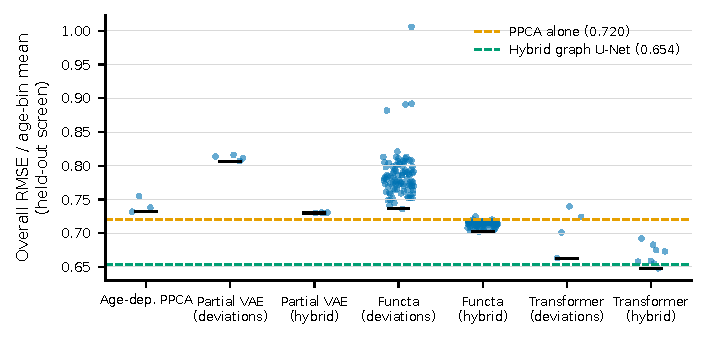
\includegraphics[width=0.75\textwidth]{figures/fig_screens.pdf}
\caption{Quick held-out screen: overall error of every screened configuration (dots; bar: best) with PPCA alone and the
hybrid graph U-Net on the same split.}\label{fig:screens}
\end{figure}

\begin{figure}[h]
\centering
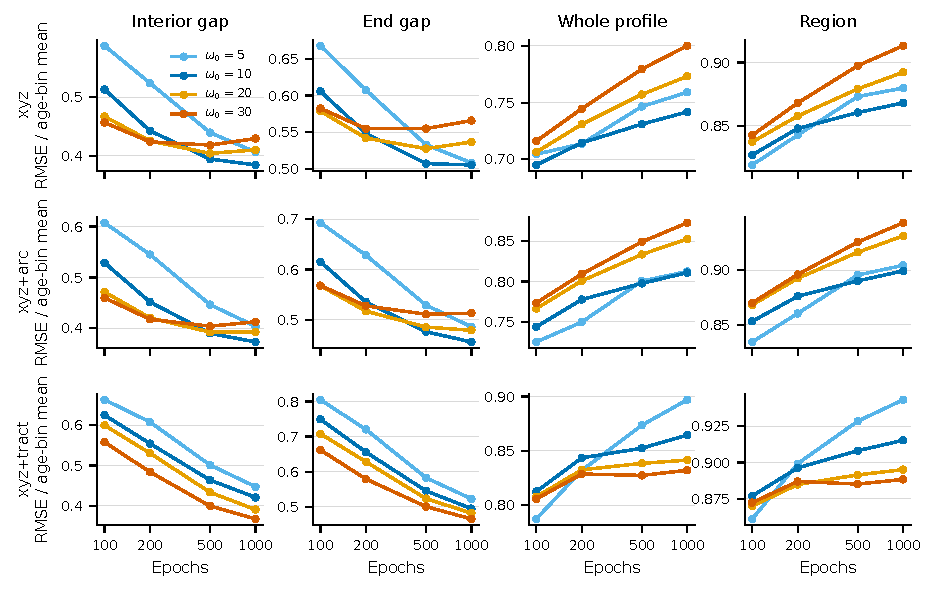
\includegraphics[width=\textwidth]{figures/fig_siren_grid.pdf}
\caption{SIREN on the deviations from the age-bin norm: error against epochs per input (rows), $\omega_0$ (colours) and
pattern (columns). Earlier protocol: 30 scans, one seed, 11 measures.}\label{fig:sirengrid}
\end{figure}

\begin{figure}[h]
\centering
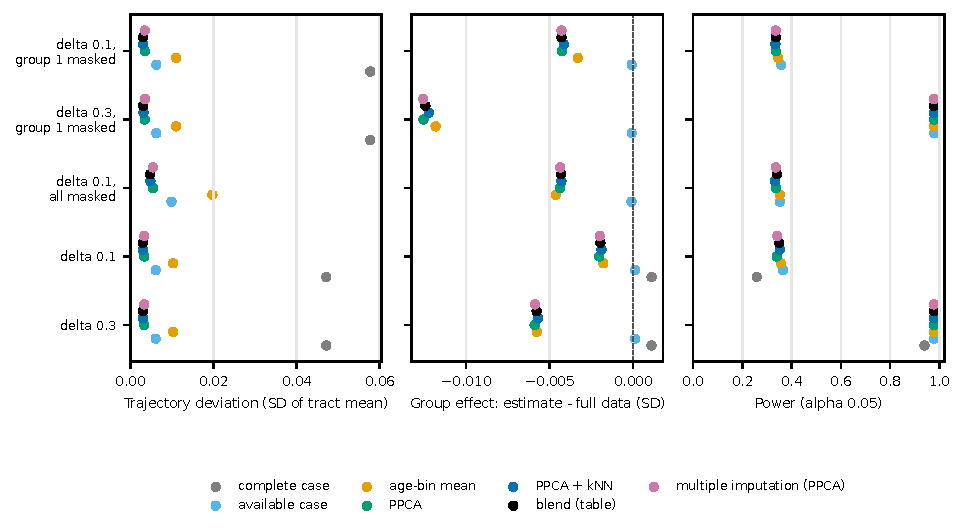
\includegraphics[width=\textwidth]{figures/fig_e4.pdf}
\caption{E4: trajectory deviation from the complete-data curve, group-effect estimate minus the complete-data estimate (between-scan SD), and power per imputer and
scenario.}\label{fig:e4}
\end{figure}

\begin{table}[h]
\centering\footnotesize
\caption{O1 and O3: norm and PPCA fitted on a share of the training subjects (learning curve) or with 7 finer age bins,
scored on the hidden values of the validation (relative to the 3-bin age-bin mean; paired whole-profile ratio against
the full training set with the 95\% subject-bootstrap CI). Seeds completed: \oOneSeeds.}\label{tab:o1o3}
\resizebox{\textwidth}{!}{\begin{tabular}{llrcccccc}
\toprule
Norm and PPCA from & Method & Training scans & Overall & Gap & End & Whole & Region & Whole: paired vs 100\% \\
\midrule
25\% of training subjects & PPCA & 99 & 0.898 & 0.817 & 0.976 & 0.878 & 0.919 & 1.167 [1.140, 1.196] \\
25\% of training subjects & PPCA + kNN & 99 & 0.835 & 0.689 & 0.865 & 0.857 & 0.927 & 1.187 [1.151, 1.226] \\
50\% of training subjects & PPCA & 198 & 0.793 & 0.738 & 0.854 & 0.769 & 0.812 & 1.067 [1.052, 1.083] \\
50\% of training subjects & PPCA + kNN & 198 & 0.719 & 0.610 & 0.724 & 0.734 & 0.806 & 1.073 [1.056, 1.094] \\
75\% of training subjects & PPCA & 295 & 0.754 & 0.704 & 0.806 & 0.729 & 0.775 & 1.021 [1.013, 1.029] \\
75\% of training subjects & PPCA + kNN & 295 & 0.681 & 0.583 & 0.683 & 0.691 & 0.768 & 1.022 [1.013, 1.031] \\
100\% of training subjects & PPCA & 395 & 0.733 & 0.684 & 0.775 & 0.712 & 0.760 & -- \\
100\% of training subjects & PPCA + kNN & 395 & 0.664 & 0.567 & 0.659 & 0.675 & 0.753 & -- \\
7 finer age bins & norm alone & 395 & 0.951 & 0.937 & 0.968 & 0.946 & 0.954 & -- \\
7 finer age bins & PPCA & 395 & 0.763 & 0.713 & 0.811 & 0.740 & 0.788 & 1.029 [1.015, 1.043] \\
7 finer age bins & PPCA + kNN & 395 & 0.694 & 0.588 & 0.696 & 0.708 & 0.786 & 1.035 [1.020, 1.051] \\
\bottomrule
\end{tabular}
}
\end{table}

\begin{figure}[h]
\centering
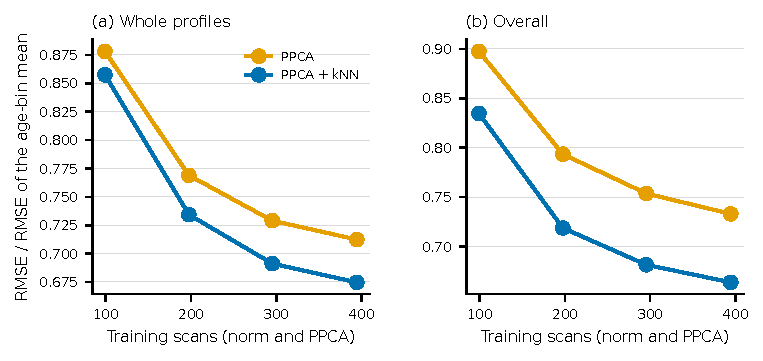
\includegraphics[width=0.7\textwidth]{figures/fig_o1o3.pdf}
\caption{O1: error of PPCA and PPCA + $k$NN against the number of normative training scans (norm and PPCA fitted on the
same subset).}\label{fig:o1o3}
\end{figure}

\begin{table}[h]
\centering\footnotesize
\caption{Quick held-out screen (one split, 30 test subjects, 2 rounds; 7 measures): best result per family and target,
selected on the test split itself; ``Runs'': configurations and test-time variants screened. Not comparable with
Table~\ref{tab:main}.}\label{tab:screens}
\setlength{\tabcolsep}{4pt}
\begin{tabular}{llrcccccccc}
\toprule
Model & Target & Runs & Overall & Gap & End & Whole & Region & Tensor & NODDI \\
\midrule
PPCA ($q=80$) & -- & 1 & 0.720 & 0.665 & 0.780 & 0.702 & 0.732 & 0.683 & 0.774 \\
Age-dependent PPCA & -- & 3 & 0.732 & 0.685 & 0.792 & 0.712 & 0.737 & 0.704 & 0.783 \\
Partial VAE & deviations & 4 & 0.807 & 0.783 & 0.844 & 0.798 & 0.801 & 0.803 & 0.885 \\
Partial VAE & PPCA correction & 4 & 0.730 & 0.673 & 0.789 & 0.712 & 0.745 & 0.696 & 0.786 \\
Functa & deviations & 93 & 0.736 & 0.674 & 0.752 & 0.730 & 0.787 & 0.692 & 0.836 \\
Functa & PPCA correction & 94 & 0.702 & 0.641 & 0.750 & 0.689 & 0.728 & 0.671 & 0.761 \\
Graph U-Net & PPCA correction & 1 & 0.654 & 0.570 & 0.678 & 0.658 & 0.711 & 0.483 & 0.672 \\
Transformer & deviations & 4 & 0.663 & 0.556 & 0.641 & 0.718 & 0.737 & 0.452 & 0.658 \\
Transformer & PPCA correction & 8 & 0.648 & 0.537 & 0.640 & 0.697 & 0.720 & 0.433 & 0.639 \\
\bottomrule
\end{tabular}

\end{table}
\begin{table}[h]
\centering\footnotesize
\caption{Error relative to the age-bin mean per measure (four patterns, mean over age bins and seeds), and for a whole
missing family. $^{\ddagger}$First row: absolute RMSE of the age-bin mean (FA, NDI, ODI, FWF $\times10^{3}$; MD, RD, AD
$\times10^{6}$\,mm$^2$/s).}\label{tab:metric}
\setlength{\tabcolsep}{5pt}
\begin{tabular}{lccccccc}
\toprule
Setting & FA & MD & RD & AD & NDI & ODI & FWF \\
\midrule
Age-bin mean: absolute RMSE$^{\ddagger}$ & 46.3 & 102.6 & 101.6 & 125.8 & 65.5 & 51.8 & 56.2 \\
\midrule
Phase 2: SIREN on deviations & 0.688 & 0.638 & 0.628 & 0.714 & 0.613 & 0.768 & 0.769 \\
PPCA alone & 0.784 & 0.657 & 0.652 & 0.756 & 0.659 & 0.818 & 0.808 \\
PPCA + SIREN & 0.663 & 0.533 & 0.533 & 0.639 & 0.535 & 0.705 & 0.689 \\
U-Net alone & 0.698 & 0.604 & 0.599 & 0.695 & 0.605 & 0.760 & 0.753 \\
Transformer alone (400) & 0.668 & 0.572 & 0.570 & 0.648 & 0.563 & 0.699 & 0.705 \\
Released default (table blend) & 0.610 & 0.504 & 0.504 & 0.587 & 0.505 & 0.645 & 0.631 \\
With HBCD reference (table blend) & 0.578 & 0.480 & 0.478 & 0.559 & 0.481 & 0.610 & 0.594 \\
\midrule
\multicolumn{8}{l}{\textit{Whole family missing (tensor: FA--AD; NODDI: NDI--FWF)}} \\
PPCA alone & 0.757 & 0.648 & 0.639 & 0.741 & 0.758 & 0.832 & 0.803 \\
U-Net alone & 0.523 & 0.512 & 0.502 & 0.585 & 0.729 & 0.680 & 0.700 \\
Transformer alone (400) & 0.490 & 0.374 & 0.379 & 0.456 & 0.681 & 0.616 & 0.573 \\
Released default (table blend) & 0.490 & 0.374 & 0.379 & 0.455 & 0.678 & 0.615 & 0.574 \\
\bottomrule
\end{tabular}

\end{table}
\begin{table}[h]
\centering\footnotesize
\caption{Absolute RMSE (four patterns; mean over patterns and seeds) per age bin; FA, NDI, ODI, FWF $\times10^{3}$,
MD, RD, AD $\times10^{6}$\,mm$^2$/s. Released default and HBCD-reference blend cross-fitted. All main settings, pooled
over age bins: Appendix Table~\ref{tab:absall}.}\label{tab:absolute}
\setlength{\tabcolsep}{4pt}
\begin{tabular}{llccccccc}
\toprule
Age bin & Setting & FA & MD & RD & AD & NDI & ODI & FWF \\
\midrule
0--3 mo & Age-bin mean & 46.0 & 121.9 & 122.5 & 138.6 & 68.1 & 66.1 & 63.0 \\
 & Released default & 26.0 & 57.9 & 56.2 & 80.9 & 37.0 & 40.1 & 41.1 \\
 & With HBCD reference & 24.2 & 51.9 & 50.0 & 74.1 & 33.5 & 36.1 & 37.1 \\
\addlinespace[2pt]
4--9 mo & Age-bin mean & 40.5 & 91.3 & 87.5 & 117.7 & 58.8 & 42.0 & 51.1 \\
 & Released default & 26.6 & 44.6 & 44.2 & 65.6 & 30.4 & 28.1 & 31.0 \\
 & With HBCD reference & 25.4 & 44.3 & 43.7 & 64.2 & 29.8 & 27.3 & 30.1 \\
\addlinespace[2pt]
10--60 mo & Age-bin mean & 52.4 & 94.5 & 94.8 & 121.1 & 69.7 & 47.3 & 54.5 \\
 & Released default & 31.4 & 52.0 & 51.7 & 75.3 & 32.0 & 30.1 & 35.0 \\
 & With HBCD reference & 30.0 & 50.2 & 49.7 & 72.5 & 31.4 & 29.0 & 33.4 \\
\bottomrule
\end{tabular}

\end{table}
\begin{table}[h]
\centering\footnotesize
\caption{Selected paired contrasts, four patterns, 162 scan $\times$ seed pairs (96 subjects): geometric mean ratio of
per-scan errors (compared / reference), 95\% CIs over pairs and from the subject-level bootstrap, Holm-adjusted Wilcoxon
$p$ (pairs / subject means), and the share of pairs where the compared setting is better.}\label{tab:paired}
\setlength{\tabcolsep}{3pt}
\resizebox{\textwidth}{!}{\begin{tabular}{llcccc}
\toprule
Contrast (compared vs reference) & Ratio & 95\% CI (pairs) & 95\% CI (subjects) & $p_\mathrm{Holm}$ (pairs / subjects) & Better \\
\midrule
\multicolumn{6}{l}{\textit{Population model}} \\
\quad PPCA + SIREN vs PPCA alone & 0.834 & 0.827--0.841 & 0.827--0.842 & $<10^{-26}$ / $<10^{-15}$ & 100\% \\
\quad PPCA + kNN vs PPCA + SIREN & 1.082 & 1.075--1.088 & 1.074--1.089 & $<10^{-26}$ / $<10^{-15}$ & 1\% \\
\quad $q=40$ vs $q=80$ (+ SIREN) & 1.008 & 1.002--1.014 & 1.002--1.014 & 0.036 / 0.008 & 42\% \\
\quad $q=120$ vs $q=80$ (+ SIREN) & 1.010 & 1.003--1.017 & 1.002--1.017 & $<10^{-4}$ / 4.3$\times10^{-4}$ & 36\% \\
\addlinespace[2pt]
\multicolumn{6}{l}{\textit{Graph U-Net}} \\
\quad U-Net alone vs PPCA + SIREN & 1.085 & 1.075--1.095 & 1.074--1.096 & $<10^{-23}$ / $<10^{-14}$ & 7\% \\
\quad U-Net beyond 4\,mm vs PPCA beyond & 0.993 & 0.990--0.995 & 0.990--0.996 & $<10^{-7}$ / $<10^{-5}$ & 70\% \\
\quad U-Net blend 0.25/0.75 vs PPCA + SIREN & 0.966 & 0.963--0.970 & 0.962--0.970 & $<10^{-25}$ / $<10^{-15}$ & 95\% \\
\addlinespace[2pt]
\multicolumn{6}{l}{\textit{Transformer}} \\
\quad Transformer alone vs PPCA + SIREN & 1.059 & 1.050--1.069 & 1.050--1.069 & $<10^{-20}$ / $<10^{-14}$ & 13\% \\
\quad Transformer alone vs U-Net alone & 0.976 & 0.970--0.983 & 0.970--0.983 & $<10^{-9}$ / $<10^{-6}$ & 74\% \\
\quad Transformer blend 0.25/0.75 vs PPCA + SIREN & 0.947 & 0.944--0.950 & 0.943--0.950 & $<10^{-26}$ / $<10^{-15}$ & 100\% \\
\quad Transformer blend vs U-Net blend (0.25/0.75) & 0.980 & 0.978--0.982 & 0.977--0.982 & $<10^{-24}$ / $<10^{-15}$ & 94\% \\
\addlinespace[2pt]
\multicolumn{6}{l}{\textit{Blending}} \\
\quad Precision weights vs fixed 0.25/0.75 & 1.012 & 1.010--1.015 & 1.010--1.015 & $<10^{-12}$ / $<10^{-9}$ & 24\% \\
\quad 400 vs 200 epochs (fixed blend) & 0.988 & 0.986--0.990 & 0.986--0.990 & $<10^{-22}$ / $<10^{-12}$ & 88\% \\
\quad Weight table vs fixed (400 epochs) & 0.987 & 0.984--0.989 & 0.984--0.989 & $<10^{-19}$ / $<10^{-11}$ & 87\% \\
\quad Released default vs PPCA + SIREN & 0.923 & 0.918--0.928 & 0.917--0.928 & $<10^{-26}$ / $<10^{-15}$ & 99\% \\
\addlinespace[2pt]
\multicolumn{6}{l}{\textit{Not helpful}} \\
\quad Acquisition correction vs none & 1.001 & 0.999--1.004 & 0.999--1.004 & 0.45 / 0.15 & 48\% \\
\addlinespace[2pt]
\multicolumn{6}{l}{\textit{Second cohort}} \\
\quad Pooled PPCA + SIREN vs BCP alone & 1.029 & 1.015--1.043 & 1.014--1.044 & $<10^{-5}$ / $<10^{-5}$ & 31\% \\
\quad Reference transformer vs BCP transformer (alone) & 0.923 & 0.913--0.933 & 0.911--0.934 & $<10^{-22}$ / $<10^{-13}$ & 93\% \\
\quad Reference vs BCP transformer (table blend) & 0.952 & 0.945--0.959 & 0.943--0.960 & $<10^{-22}$ / $<10^{-12}$ & 92\% \\
\bottomrule
\end{tabular}
}
\end{table}
\begin{figure}[h]
\centering
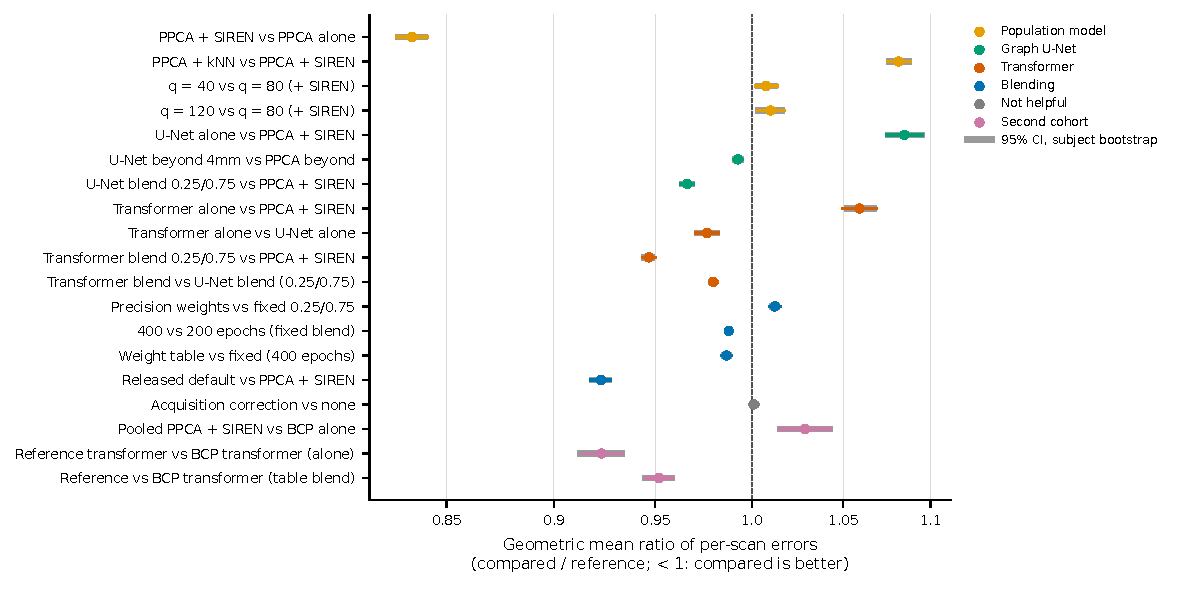
\includegraphics[width=0.8\textwidth]{figures/fig_paired.pdf}
\caption{Paired contrasts of Table~\ref{tab:paired}: geometric mean ratio (dot), 95\% CI over pairs (coloured line) and
subject-level bootstrap CI (grey bar).}\label{fig:paired}
\end{figure}
\begin{table}[h]
\centering\footnotesize
\caption{Pooling per age bin (paired, compared / reference, 95\% subject-bootstrap CI; seeds 0--2, BCP
scans).}\label{tab:poolbins}
\resizebox{\textwidth}{!}{\begin{tabular}{lcccc}
\toprule
Contrast (compared vs reference) & All & 0--3 mo & 4--9 mo & 10--60 mo \\
\midrule
Pooled PPCA + SIREN vs BCP PPCA + SIREN & 1.029 [1.014, 1.044] & 0.977 [0.939, 1.011] & 1.057 [1.035, 1.082] & 1.039 [1.025, 1.052] \\
Pooled fixed blend vs released default & 0.998 [0.985, 1.010] & 0.957 [0.923, 0.986] & 1.024 [1.008, 1.043] & 1.002 [0.994, 1.010] \\
Pooled fixed blend vs HBCD-reference fixed blend & 1.016 [1.008, 1.024] & 0.993 [0.971, 1.011] & 1.029 [1.018, 1.042] & 1.019 [1.013, 1.026] \\
HBCD-reference transformer vs BCP transformer (both 200 ep.) & 0.889 [0.877, 0.900] & 0.865 [0.833, 0.895] & 0.905 [0.891, 0.922] & 0.889 [0.878, 0.900] \\
HBCD-reference fixed blend vs BCP fixed blend (both 200 ep.) & 0.957 [0.952, 0.963] & 0.938 [0.923, 0.952] & 0.969 [0.962, 0.977] & 0.960 [0.955, 0.965] \\
Mean of BCP and reference transformers vs BCP (fixed, 400 ep.) & 0.974 [0.970, 0.977] & 0.957 [0.948, 0.965] & 0.981 [0.978, 0.985] & 0.978 [0.975, 0.981] \\
\bottomrule
\end{tabular}
}
\end{table}

\begin{table}[h]
\centering\footnotesize
\caption{E2: real-mask pattern with all donors, all settings of the validation runs (BCP: E1 and the BCP-alone run of
E5; HBCD: E3).}\label{tab:realall}
\resizebox{\textwidth}{!}{\begin{tabular}{lccc}
\toprule
Setting & BCP, untouched subjects (E1) & BCP, seeds 0--2 (E5i) & HBCD (E3) \\
\midrule
age-bin mean & 1.000 & -- & 1.000 \\
PPCA alone & 0.801 & 0.751 & 1.097 \\
PPCA + kNN & 0.758 & 0.742 & 1.083 \\
PPCA + SIREN & 0.777 & 0.753 & 1.086 \\
Transformer alone & 0.757 & -- & 0.767 \\
Fixed blend (SIREN base) & 0.723 & -- & 0.816 \\
Fixed blend (kNN base) & 0.718 & -- & 0.818 \\
Precision blend & 0.724 & -- & 0.901 \\
Shipped table (SIREN base; released default) & 0.713 & -- & 0.799 \\
Shipped table (kNN base) & 0.716 & -- & 0.805 \\
\bottomrule
\end{tabular}
}
\end{table}

\begin{table}[h]
\centering\footnotesize
\caption{Real-mask pattern by donor load (tracts missing in the donor; all donors), with the share of the real-mask
cells; error relative to the age-bin mean.}\label{tab:realload}
\resizebox{\textwidth}{!}{\begin{tabular}{llrccccc}
\toprule
Cohort & Donor missing tracts & Cells (\%) & PPCA + $k$NN & PPCA + SIREN & Transformer alone & Shipped table (released default) & Table refitted on the cohort (cross-fitted) \\
\midrule
BCP (E1) & 1 & 19 & 0.746 & 0.753 & 0.754 & 0.693 & 0.694 \\
 & 2--5 & 30 & 0.756 & 0.768 & 0.738 & 0.690 & 0.690 \\
 & 6--15 & 17 & 0.794 & 0.813 & 0.787 & 0.746 & 0.746 \\
 & 16--34 & 23 & 0.677 & 0.712 & 0.694 & 0.656 & 0.656 \\
 & $\geq$35 & 10 & 0.827 & 0.833 & 0.765 & 0.759 & 0.762 \\
\midrule
HBCD (E3) & 1 & 2 & 1.217 & 1.201 & 0.853 & 0.891 & 0.840 \\
 & 2--5 & 15 & 0.969 & 0.972 & 0.775 & 0.794 & 0.768 \\
 & 6--15 & 28 & 0.915 & 0.919 & 0.699 & 0.721 & 0.690 \\
 & 16--34 & 19 & 0.916 & 0.922 & 0.751 & 0.762 & 0.742 \\
 & $\geq$35 & 36 & 1.449 & 1.454 & 0.829 & 0.884 & 0.829 \\
\bottomrule
\end{tabular}
}
\end{table}

\end{document}
